\documentclass{article}

\usepackage{coursenotes}

\set{AuthorName}{TC Fraser}
\set{Email}{tcfraser@tcfraser.com}
\set{Website}{www.tcfraser.com}
\set{ClassName}{Topics in Condensed Matter}
\set{School}{University of Waterloo}
\set{CourseCode}{Phys 435}
\set{InstructorName}{Anton Burkov}
\set{Term}{Winter 2017}
\set{Version}{1.0}

\setfancyvecbold
\draftprofile[TC Fraser]{TC}{Red}

\begin{document}

\titlePage

\tableOfContents

\disclaimer

\section{Introduction}

The \textit{condensed} in condensed matter physics refers to the fact that a \textit{condensed} material is anything that is not a gas (i.e. liquid or solids). In this class we will be mostly interested in solids. The main qualifying feature of solids are their rigidity, (i.e. a solid has not only a fixed volume, like a liquid, but also a fixed shape). Rigidity is a consequence of the fact that atoms in solids form an ordered crystal lattice. Localized to each atom is a bunch of electrons; some in inner orbitals and some in the outer orbitals. Electrons in outer orbitals may be weakly bound to their respective atoms and be able to move around the lattice structure. These electrons are called \term{valence electrons}.

\section{Effects of the Electronic Structure Topology}

\subsection{Toy Model of a Solid}
\label{sec:toy_model}

A large part of solid state physics is related to the motion of valence electrons in a periodic potential of ionized atoms of the crystal lattice. Consider the simplest toy model of a solid: a one dimensional material with uniform spacing among the electrons with periodic potential. Let the uniform spacing between neighboring electrons be denoted $a$ and we refer the region within distance $a/2$ of each atom as the \term{primitive unit cell} or simply unit cell of the lattice. In this model (an in most of the lattice models considered in the class) we will have the working assumption that each electron is localized to an atom. This can be understood if the periodic potential $V\br{x}$ is very large between the atoms and nearly zero at the location of each atom.

\begin{center}
    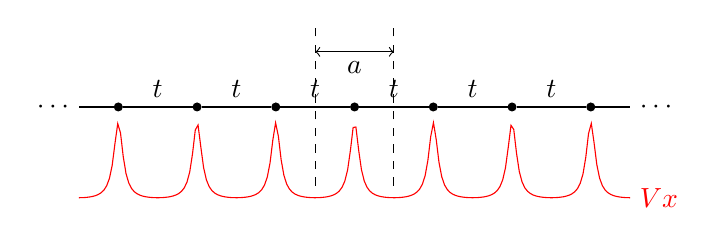
\begin{tikzpicture}
        \foreach \i in {1,...,7}
        {
            \node[draw, fill, circle, inner sep=1pt] (\i) at (\i,0) {};
        }
        \draw[] (1) -- node[above]{$t$} (2);
        \draw[] (2) -- node[above]{$t$} (3);
        \draw[] (3) -- node[above]{$t$} (4);
        \draw[] (4) -- node[above]{$t$} (5);
        \draw[] (5) -- node[above]{$t$} (6);
        \draw[] (6) -- node[above]{$t$} (7);

        \draw[] (1) -- ++(-0.5, 0) node[left]{$\cdots$};
        \draw[] (7) -- ++(+0.5, 0) node[right]{$\cdots$};

        \draw[dashed] (3.5, -1) -- (3.5, 1);
        \draw[dashed] (4.5, -1) -- (4.5, 1);
        \draw[<->] (3.5, +0.7) -- node[below]{$a$} (4.5, +0.7);
        \draw[scale=1.0,domain=0.5:7.5,samples=200,variable=\x,red] plot ({\x},{0.05/((cos(deg(pi*(\x+1/2))))^2 + 0.05) - 1.2}) node[right]{$V\br{x}$};
    \end{tikzpicture}
\end{center}


Now consider an electron moving in this potential. Quantum mechanically we anticipate any electron motion to be due to the effects of quantum tunneling. Specifically, the is expected that if an electron were to tunnel at all, it would be most likely to tunnel to its nearest neighboring atoms with some amplitude $t$. If we let $\ket{n}$ denote the state of an electron localized to the $n$-th atom ($n \in \Z$) at position $na$ in this lattice we can consider two possible ways any electron can tunnel away from $\ket{n}$.

\begin{alignat*}{2}
    \ket{n} &\stackrel{t}{\longrightarrow} \ket{n+1} \quad &&\text{transition to the right} \\
    \ket{n} &\stackrel{t}{\longrightarrow} \ket{n-1} \quad &&\text{transition to the left}
\end{alignat*}

Therefore, one can write the Hamiltonian for this system as follows,
\[ H = -t \sum_{n}\br{\underbrace{\ket{n+1}\bra{n}}_{\longrightarrow} + \underbrace{\ket{n-1}\ket{n}}_{\longleftarrow}} \eq \label{eq:toy_hamiltonian}\]
Where the preceding minus is simply convention. Notice that we are omitting the localized terms in this Hamiltonian because we can take the potential energy to be zero.
\[ \bramidket{n}{H}{n} = \bramidket{n}{V}{n} = 0 \qquad \text{Since $V\br{na} \defined 0$} \]

In order to find the energy eigenstates of the Hamiltonian \cref{eq:toy_hamiltonian} we need to find states $\ket{\psi}$ such that $H \ket{\psi} = E \ket{\psi}$. Evidently, \cref{eq:toy_hamiltonian} is non-diagonal in the $\ket{n}$ basis. Instead consider a different basis indexed by $k$ such that,
\[ \ket{n} = \sum_{k} \ket{k}\braket{k}{n} \eq \label{eq:toy_basis_change}\]
If this new basis represents momentum states, then $\braket{k}{n}$ has a specific form. Motivated by free electrons, $\braket{k}{x} \propto e^{-ikx}$ we map $x$ to the position in the crystal:
\[ x \mapsto na \]
Therefore the coefficients in \cref{eq:toy_basis_change} have similar form,
\[ \braket{k}{n} \propto e^{- ikna} \eq \label{eq:toy_plane_wave}\]
The normalization factor comes from completeness,
\[ \sum_{n} \abs{\braket{n}{k}}^2 = 1 \eq \label{eq:toy_normalization}\]
Heretofore, no restrictions have been made on the range of $n$. Evidently, a real substance will possess finite, albeit many, unit cells (atoms). Let $n \in \Z$ be an integer but equip this model with periodic boundary conditions such that there are $N$ distinct position states representing the number of unit cells. This periodic boundary condition can be written as,
\[ \ket{n} = \ket{n + N} \eq \label{eq:toy_periodic_boundary}\]
Letting $\ga \in \R$ be the normalization coefficient in \cref{eq:toy_plane_wave}, \cref{eq:toy_normalization} becomes,
\[ 1 = \sum_{n=1}^{N} \abs{\ga e^{ikna}}^2 = N \ga^2 \implies \ga = \f{1}{\sqrt{N}}\]
Consequently, \cref{eq:toy_basis_change} can be written as follows,
\[ \ket{n} = \f{1}{\sqrt{N}} \sum_{k} e^{- ikna} \ket{k} \eq \label{eq:toy_fourier_transform} \]
Additionally, the periodic boundary condition of \cref{eq:toy_periodic_boundary} gives,
\[  \ket{n} =\ket{n+N} = \f{1}{\sqrt{N}} \sum_{k} e^{- ik\br{n+N}a} \ket{k} = \f{1}{\sqrt{N}} \sum_{k} e^{- ikna} \ket{k}  \]
Therefore $e^{- ikNa} = 1$ which gives,
\[ k = \f{2\pi m}{Na} \qquad m \in \Z \eq \label{eq:toy_k_discrete}\]
Therefore $k$ must be discrete. Note that this assumption was already made above when we insisted that \cref{eq:toy_basis_change} as a new basis for the same Hilbert space. In fact, \cref{eq:toy_fourier_transform} is simply a Fourier transform that is commonly called an \term{inverse lattice Fourier transform}. Additionally, combining this with dimensionality of $\ket{n}$ gives the following constraint on the values of $k$,
\[ -\f{\pi}{a} \leq k < \f{\pi}{a} \]
Effectively corresponds to demanding that there are $N$ possible distinct values of $k$.
\[ m \in \bc{ \f{-N}{2},  \f{-N+1}{2},\ldots,  \f{N-1}{2}, \f{N}{2} } \]
\[ k \in \bc{\f{2\pi}{Na} \f{-N}{2}, \f{2\pi}{Na} \f{-N+1}{2},\ldots, \f{2\pi}{Na} \f{N-1}{2},\f{2\pi}{Na} \f{N}{2} } \eq \label{eq:discrete_finite_k} \]
In order to substitute \cref{eq:toy_fourier_transform} into \cref{eq:toy_hamiltonian}, first take the dual of \cref{eq:toy_fourier_transform},
\[ \bra{n} = \f{1}{\sqrt{N}} \sum_{k} e^{ikna} \bra{k} \eq \label{eq:dual_toy_fourier_transform} \]
Therefore \cref{eq:toy_hamiltonian} becomes,
\[ H = -t\f{1}{N} \sum_{n}\sum_{k,k'}\bc{\br{e^{-ik\br{n+1}a} \ket{k}}\br{e^{ik'na} \bra{k'}} + \br{e^{-ik\br{n-1}a} \ket{k}}\br{e^{ik'a} \bra{k'}}} \]
\[ H = -t\f{1}{N} \sum_{n}\sum_{k,k'}\bc{e^{-ik\br{n+1}a}e^{ik'na} \ket{k}\bra{k'} + e^{-ik\br{n-1}a}e^{ik'a} \ket{k}\bra{k'}} \eq \label{eq:nearly_toy_diag}\]
By \cref{eq:toy_k_discrete}, $\br{k - k'}$ is an integer multiple of $2 \pi / Na$. Letting that integer be $\mu$ we have the following identity:
\[ \f{1}{N} \sum_{n=1}^{N} e^{i\br{k - k'}na} = \f{1}{N} \sum_{n=1}^{N} e^{i2 \pi \mu n / N} = \de_{\mu} = \de_{k, k'}  \eq \label{eq:crucial_idenity}\]
Therefore \cref{eq:nearly_toy_diag} simplifies greatly,
\[ H = -t \sum_{n}\sum_{k,k'} \de_{k,k'} \bc{e^{-ika} \ket{k}\bra{k'} + e^{ika} \ket{k}\bra{k'}} \]
\[ H = -t \sum_{n}\bc{e^{-ika} + e^{ika}} \ket{k}\bra{k} \]
\[ H = -2t\cos\br{ka} \sum_{n}\ket{k}\bra{k} \eq \label{eq:toy_hamiltonian_diag}\]
Therefore \cref{eq:toy_hamiltonian_diag} is the diagonalized form of \cref{eq:toy_hamiltonian}. By diagonalizing the Hamiltonian we were able to determine the energy levels $\vep\br{k}$ of the various states,
\[ \varepsilon\br{k} = - 2 t \cos\br{ka} \eq \label{eq:toy_single_energy_band}\]
The momentum space index $k$ is the wave-vector with $p = \hbar k$ where $p$ is an ordinary linear momentum. Additionally, $t$ acts as a tunneling coefficient that dictates a tunneling \textit{rate} (up to a constant $\hbar$) for the electrons in the solid. Unlike free particles, the momentum $k$ in this toy model is confined to a discrete region.
\[ -\f{\pi}{a} \leq k < \f{\pi}{a} \]
This interval is called the \term{first Brillouin zone}. To highlight this difference, we sometimes refer to $p$ in this model as the \term{crystal momentum} of the electron in state $\ket{k}$.\\

Moreover, the periodic boundary conditions restrict $k$ to take on discrete and finite values pursuant to \cref{eq:discrete_finite_k}.
Note that $L = Na$ is the size of the crystal, $N$ is the number of atoms and $a$ is the interval between two atoms in the solid.\\

The states that diagonalized the Hamiltonian are called \term{Bloch states} and are denoted $\ket{k}$ where is given by the inverse crystal Fourier transform (inverse of \cref{eq:toy_fourier_transform}),
\[ \ket{k} = \f{1}{\sqrt{N}} \sum_{n} \ket{n} e^{i k na} \]
Which is a \term{lattice Fourier transform}. Since \cref{eq:toy_single_energy_band} takes on the form of a cosine with amplitude $2t$ the accessible energy levels are confined to the finite interval,
\[ \varepsilon_{\min} = - 2t \qquad \varepsilon_{\max} = + 2t \]
The interval has a width of $\varepsilon_{\max} - \varepsilon_{\min} = 4t$ and is referred to as the allowed energy \textit{band}.

\begin{center}
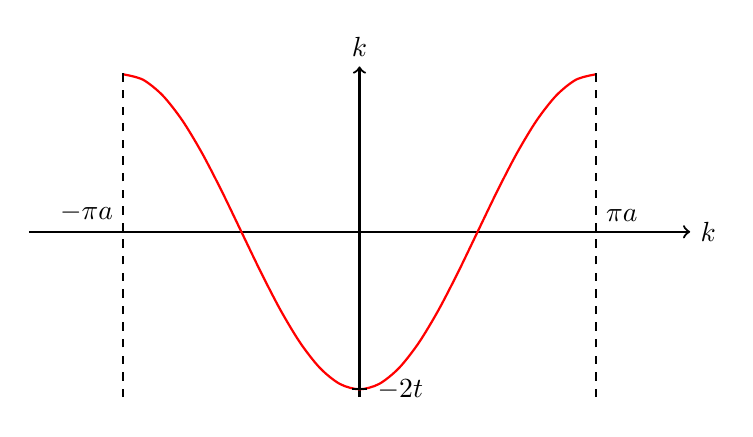
\begin{tikzpicture}
    \pgfmathsetmacro{\axissize}{2.1};
    \pgfmathsetmacro{\plotsize}{3};
    \draw[thick,->] (-2*\axissize,0) -- (+2*\axissize,0) node[right]{$k$};
    \draw[thick,->] (0, -\axissize) -- (0,+\axissize) node[above]{$\vep\br{k}$};
    \draw[thick,scale=1.0,domain=-pi:pi,smooth,variable=\k,red] plot ({\k/pi*\plotsize},{-2*cos(deg(\k))});
    \draw[thick,dashed] (\plotsize, -\axissize) -- node[above right]{$\f{\pi}{a}$} (\plotsize,+\axissize);
    \draw[thick,dashed] (-\plotsize, -\axissize) -- node[above left]{$-\f{\pi}{a}$} (-\plotsize,+\axissize);
    \draw[thick,-] (-0.1,-2) -- (+0.1,-2) node[right]{$-2t$};
\end{tikzpicture}
\end{center}

Given \cref{eq:discrete_finite_k}, there are $N$ distinct Bloch vector states $\ket{k}$. Suppose now that we have $1$ electron per atom (instead of $1$ electron in total). We recall the \term{Pauli principle} which states that only $1$ electron can occupy a given state in a band. If there is one electron per atom and $N$ total atoms, there are $N$ electrons. If we recall the fact that electrons are spin-$1/2$ fermions, each momentum state corresponds to two distinct spin states. Therefore in total there are $2N$ states accessible to the electrons and therefore the band is \textit{half-filled}.
\begin{center}
\begin{tikzpicture}
    \pgfmathsetmacro{\axissize}{4};
    \pgfmathsetmacro{\plotsize}{3};
    \draw[->] (0,0) -- (+\axissize,0) node[right]{$T$};
    \draw[->] (0, 0) -- (0,+\axissize) node[above]{$\rho\br{T}$};
    \draw[scale=1.0,domain=0.25:\plotsize,smooth,variable=\T,red] plot ({\T},{1/\T});
\end{tikzpicture}
\end{center}

Of course, this holds when the electrons in the material are at zero temperature where the electrons occupy all of the lowest possible energy states. For a half-filled energy band, all of the \textit{negative} energy states are filled and the positive energy states are vacant. This separation defines the \term{Fermi energy} for this system which occurs at the interface between filled energy states and un-filled energy states ($\vep\tsb{F} = 0$ in this problem). In order to find the state that corresponds to this upper limit one needs to solve,
\[ \vep\br{k} = \vep\tsb{F} = 0 \implies -2t \cos\br{ka} = 0 \]
Therefore the value of $k$ that solves this equation is,
\[  k = \pm \f{\pi}{2a} = \pm k\tsb{F}\]
Where $k\tsb{F}$ is given a special name: the \term{Fermi wave-vector} (Fermi momentum).
\begin{align*}
    \abs{k} < k\tsb{F} &: \text{filled states}\\
    \abs{k} > k\tsb{F} &: \text{empty states}
\end{align*}
The \term{Fermi surface} defines the surface in momentum space separating the filled states from the unfilled states. Most of the observed properties of metals follow from the existence of the Fermi surface. \\

This concept is so important that it is worth measuring the volume \text{in momentum space} corresponding to the filled states. This is the volume enclosed by the Fermi surface. In this example, the volume in momentum space is characterized by the $2 k\tsb{F}$ interval. Since $k = 2\pi m / Na$, the volume per single $k$-value is $2 \pi / Na$. Letting $n = 1/a$ be the linear density of electrons per unit length, we can compute the total number of electrons:
\[ N =  n N a = 2 \f{2k\tsb{F}}{2 \pi / Na} \]
Which allows one to calculate $k\tsb{F}$ in terms of the electron density $n$,
\[ k\tsb{F} =\f{\pi}{2} n \]
Which makes sense for this model because there is one electron per atom making $n = 1/a$.
This result is called \term{Luttinger's theorem} which states that the volume enclosed by the Fermi surface (sometimes called the Fermi sea) is directly proportional to the electron density. \\

\subsection{Polyacetylene}

In \cref{sec:toy_model} we considered a one dimensional toy model of electrons in a solid. This model is highly idealized and is fair from a description of a real material. It is possible however to modify the model analyzed in \cref{sec:toy_model} to consider the case of the one dimensional polymer called polyacetylene. Polyacetylene consists of weakly-interacting chains of CH units.
\begin{align*}
    \text{C} &: 1s^2 2s^2 2p^2 \qquad \text{4 valence electrons}\\
    \text{H} &: 1s^1
\end{align*}

Electrons found in the inner orbitals of the atoms are tightly bound to their nuclei and therefore only the valence electrons in carbon are free to travel throughout the lattice.

\begin{center}
    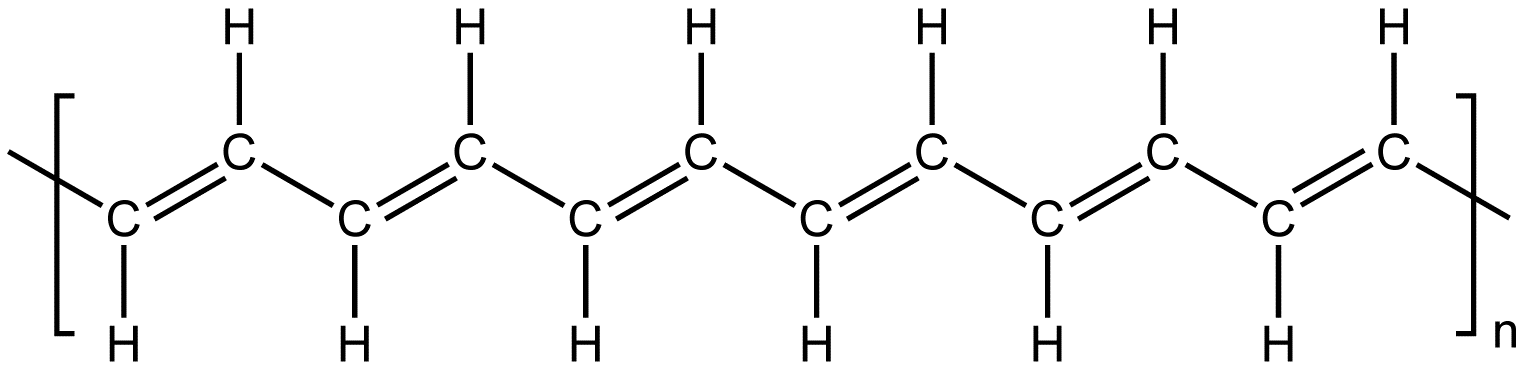
\includegraphics[width=\linewidth]{figures/polyacetylene.png}
\end{center}

Three of the valence electrons are engaged in bonding with neighboring carbon and hydrogen atoms while the $4$-th one is free to move around. As it turns out, the bonds between carbon atoms possess alternating tunneling amplitudes.

\begin{center}
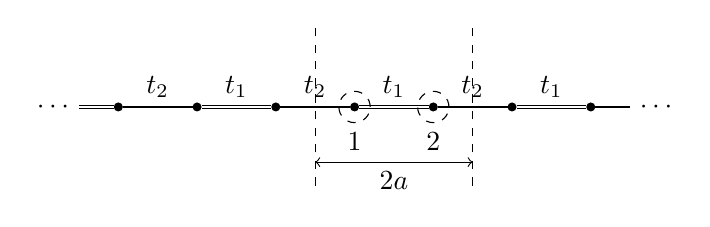
\begin{tikzpicture}
    \foreach \i in {1,...,7}
    {
        \node[draw, fill, circle, inner sep=1pt] (\i) at (\i,0) {};
    }
    \draw[]       (1) -- node[above]{$t_2$} (2);
    \draw[double] (2) -- node[above]{$t_1$} (3);
    \draw[]       (3) -- node[above]{$t_2$} (4);
    \draw[double] (4) -- node[above]{$t_1$} (5);
    \draw[]       (5) -- node[above]{$t_2$} (6);
    \draw[double] (6) -- node[above]{$t_1$} (7);

    \node[dashed, draw, circle, inner sep=4pt, label={below:$1$}] at (4,0) {};
    \node[dashed, draw, circle, inner sep=4pt, label={below:$2$}] at (5,0) {};

    \draw[double] (1) -- ++(-0.5, 0) node[left]{$\cdots$};
    \draw[]       (7) -- ++(+0.5, 0) node[right]{$\cdots$};

    \draw[dashed] (3.5, -1) -- (3.5, 1);
    \draw[dashed] (5.5, -1) -- (5.5, 1);
    \draw[<->] (3.5, -0.7) -- node[below]{$2a$} (5.5, -0.7);
\end{tikzpicture}
\end{center}
In Polyacetylene, the tunneling amplitude between the carbon atoms joined by a double bound is slightly higher $t_1 > t_2$. This is referred to as \term{Peierls instability}. \\

Since this deviation is only slight, let $2\de t = t_1 - t_2$ be a small perturbation such that,
\[ t_1 = t + \de t \qquad t_2 = t - \de t \eq \label{eq:t1t2}\]
Another important difference is that the primitive unit cell has size $2a$ (instead of $a$). This two atom basis can be arranged on a lattice with lattice constant $2a$. This is referred to as a \term{Bravais lattice}. Notationally, we can describe any crystal as,
\[ \text{crystal} = \br{\text{basis}, \text{Bravais lattice}} \]

To describe an electron in this lattice, we need two indices: one to describe the unit cell the electron is in ($n$) and one to describe which atom ($1$ or $2$) the electron is located at within the unit cell. Therefore the Hamiltonian needs to characterize a number of possible transitions,

\begin{alignat*}{2}
    \ket{n, 1} &\stackrel{t_1}{\longrightarrow} \ket{n, 2} \quad &&\text{transition to the right within a unit cell} \\
    \ket{n, 2} &\stackrel{t_1}{\longrightarrow} \ket{n, 1} \quad &&\text{transition to the left within a unit cell} \\
    \ket{n, 1} &\stackrel{t_2}{\longrightarrow} \ket{n-1, 2} \quad &&\text{transition to the left across a unit cell} \\
    \ket{n, 2} &\stackrel{t_2}{\longrightarrow} \ket{n+1, 1} \quad &&\text{transition to the right across a unit cell}
\end{alignat*}

Just as before in \cref{sec:toy_model}, we only consider the tunneling of electrons for nearest neighbors. This will be a recurring motif of this class which is formally called the \term{tight-binding model}.
\[ H = \sum_{n} \bc{ - t_1 \ket{n, 2} \bra{n, 1} - t_2 \ket{n-1, 2} \bra{n, 1} - t_1 \ket{n, 1} \bra{n, 2} - t_2 \ket{n+1, 1} \bra{n, 2}} \eq \label{eq:polyacetylene_tight_binding}\]
Just as before, we need to write $\ket{n, \al}$ in the momentum basis (a new basis for each $\al \in \bc{1,2}$),
\[ \ket{n, \al} = \sum_{k} \ket{k,\al} \braket{k, \al}{n, \al} \eq \label{eq:basis_change}\]
where $\braket{k, \al}{n, \al}$ has a specific form. Motivated by free electrons, $\braket{k}{x} \propto e^{-ikx}$ we map $x$ to the position in the crystal:
\[ x \mapsto n\cdot2a \]
Noting the factor of $2$ because the unit call is twice as long as before. The coefficients in \cref{eq:basis_change} have similar form,
\[ \braket{k, \al}{n, \al} \propto e^{- i2kna} \eq \label{eq:plane_wave}\]
The normalization factor comes from completeness,
\[ \sum_{n} \abs{\braket{n, \al}{k, \al}}^2 = 1 \eq \label{eq:normalization}\]
Analogously to \cref{sec:toy_model}, let $n \in \Z$ be an integer but equip this model with periodic boundary conditions such that there are $N$ distinct positions for the electron for each $\al \in \bc{1,2}$ representing the number of unit cells. It is important to note that here $N$ does not represent the total number of atoms; $N$ is the total number of unit cells (equivalently the total number of distinct $\ket{n, \al}$ states for \textit{fixed} $\al$). Moreover the extra factor of $2$ in the exponential is due to the increases unit cell size.
Therefore the periodic boundary conditions for each $\al$ are,
\[ \ket{n, \al} = \ket{n + N, \al} \eq \label{eq:periodic_boundary}\]
Letting $\ga \in \R$ be the normalization coefficient in \cref{eq:plane_wave}, \cref{eq:normalization} becomes,
\[ 1 = \sum_{n=1}^{N} \abs{\ga e^{i2kna}}^2 = N \ga^2 \implies \ga = \f{1}{\sqrt{N}}\]
Consequently, \cref{eq:basis_change} can be written as follows,
\[ \ket{n, \al} = \f{1}{\sqrt{N}} \sum_{k} e^{- i2kna} \ket{k, \al}  \]
Additionally, the periodic boundary condition of \cref{eq:periodic_boundary} gives,
\[  \ket{n, \al} =\ket{n+N, \al} = \f{1}{\sqrt{N}} \sum_{k} e^{- i2k\br{n+N}a} \ket{k, \al} = \f{1}{\sqrt{N}} \sum_{k} e^{- i2kna} \ket{k, \al}  \]
Therefore $e^{- i2kNa} = 1$ which gives,
\[ k = \f{\pi m}{Na} \qquad m \in \Z \eq \label{eq:k_discrete}\]
Therefore $k$ must be discrete (an assumption made above to write down \cref{eq:basis_change}). Additionally, combining this with dimensionality of $\ket{n, \al}$ gives the following constraint on $k$,
\[ \f{\pi}{2a} \leq k < \f{\pi}{2a} \]
Note the Brillouin zone for Polyacetylene is half the width of the Brillouin zone for the toy model discussed in \cref{sec:toy_model} (again this is due to the unit cell being twice the size). Thus ensures there are $N$ states of the form $\ket{k, \al}$. \\

Substituting these results into \cref{eq:polyacetylene_tight_binding} gives,
\begin{align*}
\eq \label{eq:H_polyacetylene}
\begin{split}
H
&= - t_1 \f{1}{N} \sum_{n} \sum_{k ,k'} \ket{k, 2}\bra{k', 1} e^{-2ikna}e^{2ik'na} \\
&\quad  - t_2 \f{1}{N} \sum_{n} \sum_{k ,k'} \ket{k, 2}\bra{k', 1} e^{-2ik\br{n-1}a}e^{2ik'na} \\
&\quad  - t_1 \f{1}{N} \sum_{n} \sum_{k ,k'} \ket{k, 1}\bra{k', 2} e^{-2ikna}e^{2ik'na} \\
&\quad  - t_2 \f{1}{N} \sum_{n} \sum_{k ,k'} \ket{k, 1}\bra{k', 2} e^{-2ikna}e^{2ik'\br{n-1}a}
\end{split}
\end{align*}
\begin{align*}
    \eq \label{eq:H_energy_difference_ks_diag}
    \begin{split}
    H
    &= \f{1}{N}\sum_{n} \sum_{k_1, k_2} \ket{k_1, 1}\bra{k_2, 2} \bc{-t_1 e^{i2\br{k_2 - k_1}na} - t_2 e^{- i2k_1a}e^{i2\br{k_2 - k_1}na}}+ \cdots\\
    &\cdots + \f{1}{N}\sum_{n} \sum_{k_1, k_2} \ket{k_1, 2}\bra{k_2, 1} \bc{-t_1 e^{i2\br{k_2 - k_1}na} - t_2 e^{+ i2k_1a}e^{i2\br{k_2 - k_1}na}}
    \end{split}
\end{align*}
By \cref{eq:k_discrete}, $\br{k_2 - k_1}$ is an integer multiple of $\pi / Na$. Letting that integer be $\mu$ we have the following identity:
\[ \f{1}{N} \sum_{n=1}^{N} e^{i2\br{k_2 - k_1}na} = \f{1}{N} \sum_{n=1}^{N} e^{i2 \pi \mu n / N} = \de_{\mu} = \de_{k_1, k_2} \]
Therefore \cref{eq:H_energy_difference_ks_diag} simplifies greatly,
\begin{align*}
    \eq \label{eq:H_energy_difference_ks_diag_simp}
    \begin{split}
    H
    &= - t_1 \sum_{k}\bc{\ket{k ,2} \bra{k, 1} + \ket{k, 1}\bra{k,2}} \\
    &\quad - t_2 \sum_{k}\bc{\ket{k ,2} \bra{k, 1}e^{2ika} + \ket{k, 1}\bra{k,2}e^{-2ika}}
    \end{split}
\end{align*}

At this point \cref{eq:H_energy_difference_ks_diag_simp} has been diagonalized with respect to the momentum index $k$ (it is a simple sum over $k$). It is not however diagonalized completely. To diagonalize this Hamiltonian further, we can write $H = \sum_{k} H\br{k}$ where $H\br{k}$ is the summand of \cref{eq:H_energy_difference_ks_diag_simp}. Henceforth, the dependence of $k$ can be omitted from the states $\ket{k, \al}$ for convenience.

\[ H\br{k} = - \br{t_1 + t_2 e^{- i2ka} }\ket{1}\bra{2} - \br{t_1 + t_2 e^{+ i2ka} }\ket{2}\bra{1} \]
Notice that $H\br{k}$ can be written as a $2\times 2$ matrix as follows,
\[ H\br{k} = \kbordermatrix{ & 1 & 2 \\ 1 & 0 & - \br{t_1 + t_2 e^{- i2ka} } \\ 2 & - \br{t_1 + t_2 e^{+ i2ka} } & 0 } \eq \label{eq:H_matrix}\]
Since $H\br{k}$ represents a two level system, we can therefore write $H\br{k}$ as a sum over the three Pauli matrices with the following spin-correspondence (which we refer to as a \term{pseudo-spin}),
\[ \ket{1} = \ket{\uparrow} \qquad \ket{2} = \ket{\downarrow} \]
The \term{Pauli matrices} are,
\begin{align*}
\eq \label{eq:pauli_matrices}
\begin{split}
\si_x &= \begin{pmatrix} 0 & 1 \\ 1 & 0 \end{pmatrix} = \ket{1} \bra{2} + \ket{2} \bra{1} \\
\si_y &= \begin{pmatrix} 0 & -i \\ i & 0 \end{pmatrix} = -i\br{\ket{1} \bra{2} - \ket{2} \bra{1}} \\
\si_z &= \begin{pmatrix} 1 & 0 \\ 0 & -1 \end{pmatrix} = \ket{1} \bra{1} - \ket{2} \bra{2}
\end{split}
\end{align*}
Upon close inspection of \cref{eq:H_matrix}, it becomes easy to identity the Pauli's within $H\br{k}$. Explicitly the $t_1$ term is easy,
\[ H\br{k} = \ep \si_z - t_1 \si_x - t_2 \begin{pmatrix} 0 & e^{- i2ka} \\ e^{+ i2ka} & 0 \end{pmatrix}\]
The remaining decomposition follows from $e^{\pm ix} = \cos\br{x} \pm i \sin \br{x}$
\[ H\br{k} = \ep \si_z - t_1 \si_x - t_2 \cos\br{2 k a}\si_x - t_2 \sin\br{2 k a}\si_y \]
Alternatively it is possible to finding  this correspondence by making use of (pseudo-)ladder operators of \cref{eq:pauli_matrices},
\[ \ket{1}\bra{2} = \f{1}{2}\br{\si_x + i \si_y} \]
We therefore define $\ve d \br{k}$ as an \term{effective magnetic field} such that,
\[ \ve d\br{k} = \begin{pmatrix} d_x\br{k} \\ d_y\br{k} \\ d_z\br{k} \end{pmatrix} = \begin{pmatrix} -t_1 - t_2 \cos\br{2 k a} \\ - t_2 \sin\br{2 k a} \\ 0 \end{pmatrix} \eq \label{eq:dk}\]
Therefore $H\br{k} = \ve d\br{k} \cdot \ve \si$. This system is \textit{equivalent} to a spin-1/2 particle in a magnetic field of the form $\ve d\br{k}$. The eigenstates of $H\br{k}$ correspond to $\ba{\ve \si}$ along $\ve d$ or in the opposite direction to $\ve d$.
\[ \vep_{-}\br{k} = -\abs{\ve d \br{k}} \qquad \vep_{+}\br{k} = +\abs{\ve d \br{k}} \]
Using \cref{eq:t1t2},
\begin{align*}
\eq \label{eq:dk_alt}
\begin{split}
d_x \br{k} &= - \br{t + \de t} - \br{t - \de t} \cos\br{2 ka} \\
d_y \br{k} &= - \br{t - \de t} \sin\br{2 ka} \\
d_z \br{k} &= 0
\end{split}
\end{align*}
This is contrasting to the previous model; before we had a \textit{single} energy band pursuant to \cref{eq:toy_single_energy_band}, but here we have \textit{two energy bands}. This result can be generalized to the following observation:
\begin{center}
    \textit{Every atom in the unit cell will give rise to a separate band.}
\end{center}
Explicitly, $\abs{\ve d \br{k}}^2$ can be calculated from \cref{eq:dk_alt},
\[ \abs{\ve d \br{k}}^2 = d_x^2 \br{k} + d_y^2 \br{k} + d_z^2 \br{k} = 4 t^2 \cos^2 \br{ka} + 4 \de t^2 \sin^2 \br{ka} \]
Which makes the two bands have the form,
\[ \vep_{\pm}\br{k} = \pm 2 \sqrt{t^2 \cos^2\br{ka} + \de t^2 \sin^2\br{ka}} \]
Which when plotted is,
\begin{center}
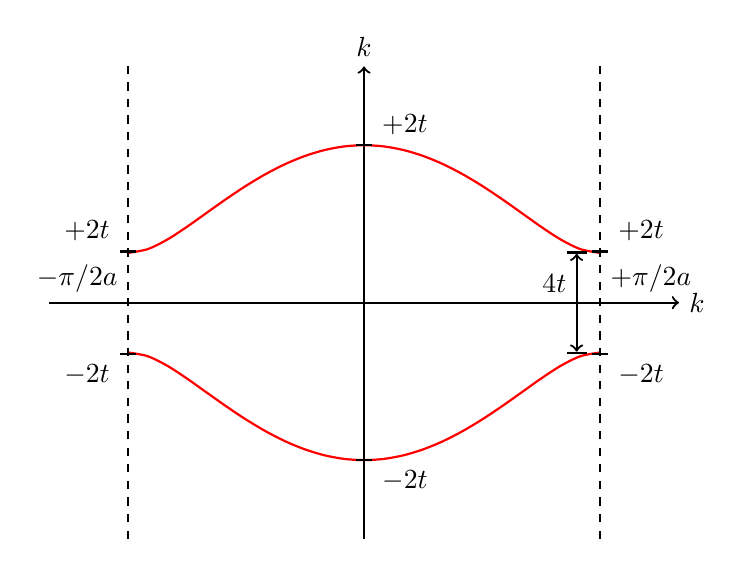
\begin{tikzpicture}
    \pgfmathsetmacro{\axissizev}{3};
    \pgfmathsetmacro{\axissizeh}{4};
    \pgfmathsetmacro{\plotsize}{3};
    \pgfmathsetmacro{\dt}{0.65};
    \draw[thick,->] (-\axissizeh,0) -- (+\axissizeh,0) node[right]{$k$};
    \draw[thick,->] (0, -\axissizev) -- (0,+\axissizev) node[above]{$\vep\br{k}$};
    \draw[thick,scale=1.0,domain=-pi/2:pi/2,smooth,variable=\k,red] plot ({2 *\k/pi*\plotsize},{-2*sqrt(cos(deg(\k))^2 + 0.1*sin(deg(\k))^2)});
    \draw[thick,scale=1.0,domain=-pi/2:pi/2,smooth,variable=\k,red] plot ({2 *\k/pi*\plotsize},{2*sqrt(cos(deg(\k))^2 + 0.1*sin(deg(\k))^2)});
    \draw[thick,dashed] (\plotsize, -\axissizev) -- node[above right]{$+{\pi}/{2a}$} (\plotsize,+\axissizev);
    \draw[thick,dashed] (-\plotsize, -\axissizev) -- node[above left]{$-{\pi}/{2a}$} (-\plotsize,+\axissizev);
    \draw[thick,] (-0.1,-2) -- (+0.1,-2) node[below right]{$-2t$};
    \draw[thick,] (-0.1,+2) -- (+0.1,+2) node[above right]{$+2t$};
    \draw[thick,] (\plotsize-0.1, \dt) -- (\plotsize+0.1, \dt) node[above right]{$+2\de t$};
    \draw[thick,] (\plotsize-0.1, -\dt) -- (\plotsize+0.1, -\dt) node[below right]{$-2\de t$};
    \draw[thick,] (-\plotsize+0.1, \dt) -- (-\plotsize-0.1, \dt) node[above left]{$+2\de t$};
    \draw[thick,] (-\plotsize+0.1, -\dt) -- (-\plotsize-0.1, -\dt) node[below left]{$-2\de t$};
    \draw[thick,|<->|] (\plotsize-0.3, \dt) -- node[above left]{$4 \de t$} (\plotsize-0.3, -\dt);
\end{tikzpicture}
\end{center}

Notice that the first Brillouin zone is $\f{\pi}{2a} \leq k \leq \f{\pi}{2a}$ is \textit{smaller} than it was previously. In this model, there is one electron per atom and thus two electrons per unit cell. Therefore there are $2N$ electrons. Accounting for spin degeneracies, there are $2N$ accessible states per energy band. At zero temperature, the entire lower band is filled and the upper band is empty. This makes polyacetylene an \term{insulator} because it requires an energy of at least $4 \de t$ in order to transition an electron across the Fermi surface. \\

In the limit of the $\de t \to 0$ one should expect to recover \cref{eq:toy_single_energy_band} from \cref{sec:toy_model},
\[ \lim_{\de t \to 0}\vep_{\pm}\br{k} = \pm 2 \lim_{\de t \to 0}\sqrt{t^2 \cos^2\br{ka} + \de t^2 \sin^2\br{ka}} = \pm 2 t \cos\br{ka}  \]
As expected. Notice however the plot of $\vep\br{k}$ when $\de t = 0$ differs from the one depicted in \cref{sec:toy_model},
\begin{center}
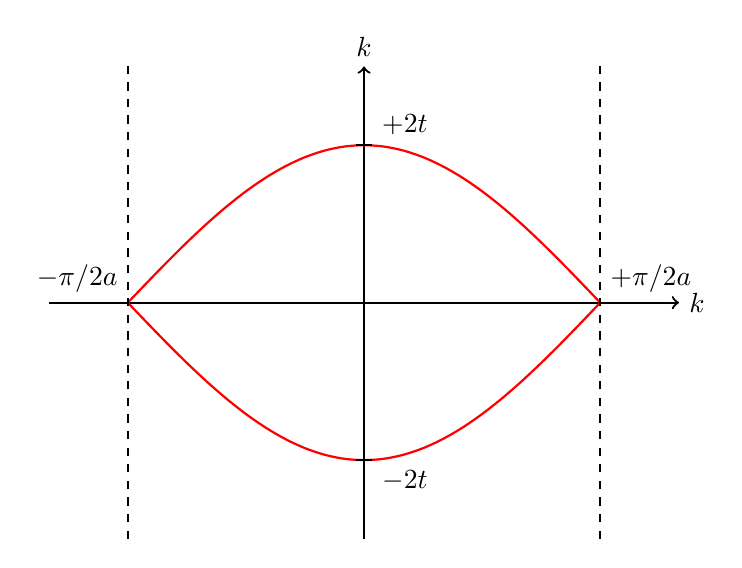
\begin{tikzpicture}
    \pgfmathsetmacro{\axissizev}{3};
    \pgfmathsetmacro{\axissizeh}{4};
    \pgfmathsetmacro{\plotsize}{3};
    \pgfmathsetmacro{\dt}{0.65};
    \draw[thick,->] (-\axissizeh,0) -- (+\axissizeh,0) node[right]{$k$};
    \draw[thick,->] (0, -\axissizev) -- (0,+\axissizev) node[above]{$\vep\br{k}$};
    \draw[thick,scale=1.0,domain=-pi/2:pi/2,smooth,variable=\k,red] plot ({2 *\k/pi*\plotsize},{-2*sqrt(cos(deg(\k))^2)});
    \draw[thick,scale=1.0,domain=-pi/2:pi/2,smooth,variable=\k,red] plot ({2 *\k/pi*\plotsize},{2*sqrt(cos(deg(\k))^2)});
    \draw[thick,dashed] (\plotsize, -\axissizev) -- node[above right]{$+{\pi}/{2a}$} (\plotsize,+\axissizev);
    \draw[thick,dashed] (-\plotsize, -\axissizev) -- node[above left]{$-{\pi}/{2a}$} (-\plotsize,+\axissizev);
    \draw[thick,] (-0.1,-2) -- (+0.1,-2) node[below right]{$-2t$};
    \draw[thick,] (-0.1,+2) -- (+0.1,+2) node[above right]{$+2t$};
\end{tikzpicture}
\end{center}
The resolution between these two plots is to notice that in the polyacetylene model, the unit cell had with $2a$ instead of $a$. Therefore in momentum space, the plotted values for $k$ are bounded by $- \pi / 2a \leq k \leq \pi / 2a$ instead of $- \pi / a \leq k \leq \pi / a$. If one were to unravel the upper band into regions where $\abs{k} > \pi / 2a$ one would recover the initial model. \\

Heretofore, we have assumed that $\de t > 0$. If however we consider $\de t< 0$, then we transition from $t_1 > t_2$ to $t_2 > t_1$ pursuant to \cref{eq:t1t2}. And our diagram is adjusted

\begin{center}
    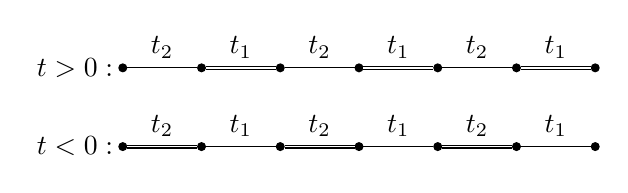
\begin{tikzpicture}
        \foreach \i in {1,...,7}
        {
            \node[draw, fill, circle, inner sep=1pt] (n\i) at (\i,0) {};
            \node[draw, fill, circle, inner sep=1pt] (p\i) at (\i,1) {};
        }
        \draw[]       (p1) -- node[above]{$t_2$} (p2);
        \draw[double] (p2) -- node[above]{$t_1$} (p3);
        \draw[]       (p3) -- node[above]{$t_2$} (p4);
        \draw[double] (p4) -- node[above]{$t_1$} (p5);
        \draw[]       (p5) -- node[above]{$t_2$} (p6);
        \draw[double] (p6) -- node[above]{$t_1$} (p7);
        \draw (p1) node[left]{$\de t > 0 : $};

        \draw[double] (n1) -- node[above]{$t_2$} (n2);
        \draw[]       (n2) -- node[above]{$t_1$} (n3);
        \draw[double] (n3) -- node[above]{$t_2$} (n4);
        \draw[]       (n4) -- node[above]{$t_1$} (n5);
        \draw[double] (n5) -- node[above]{$t_2$} (n6);
        \draw[]       (n6) -- node[above]{$t_1$} (n7);
        \draw (n1) node[left]{$\de t < 0 : $};
    \end{tikzpicture}
\end{center}

Therefore, the ground state of polyacetylene is doubly degenerate, corresponding to the two signs of $\de t$. As it turns out, this difference in sign is related to topological properties in momentum space. Upon examination of \cref{eq:dk} once can notice how $\ve d$ depends on $\de t$. How does $\ve d\br{k}$ change as $k$ goes from $- \pi / 2a$ to $\pi  2a$?
\begin{align*}
\begin{split}
d_x \br{k} &= - \br{t + \de t} - \br{t - \de t} \cos\br{2 ka} \\
d_y \br{k} &= - \br{t - \de t} \sin\br{2 ka}
\end{split}
\end{align*}
Checking specific points,
\begin{align*}
d_x \br{\pm\f{\pi}{2a}} &= - \br{t + \de t} + \br{t - \de t} = - 2 \de t\\
d_y \br{\pm\f{\pi}{2a}} &= 0 \\
d_x \br{0} &= - \br{t + \de t} - \br{t - \de t} = 2 t\\
d_y \br{0} &= 0
\end{align*}
Plotted the case of $\de t >0$ in $d_y, d_x$ space,
\begin{center}
\begin{tikzpicture}
    \pgfmathsetmacro{\axissize}{3};
    \pgfmathsetmacro{\t}{1};
    \pgfmathsetmacro{\dt}{0.1};
    \pgfmathsetmacro{\tick}{0.1};
    \draw[thick,->] (-\axissize,0) -- (+\axissize,0) node[right]{$d_x$};
    \draw[thick,->] (0, -\axissize) -- (0,+\axissize) node[above]{$d_y$};
    \draw[thick,scale=1.0,domain=-pi/2:pi/2,smooth,variable=\k,red] plot ({- (\t + \dt) - (\t - \dt)*cos(deg(2*\k))},{- (\t - \dt)*sin(deg(2*\k))});
    \draw[thick,] (-2*\t, -\tick) -- (-2*\t, \tick) node[above left]{$-2t$};
    \draw[thick,] (-2*\dt, -\tick) -- (-2*\dt, \tick) node[above left]{$-2\de t$};
    \draw[thick,] (- 2, 2) node[]{$\de t > 0$};
\end{tikzpicture}
\end{center}
It can be seen that when $\de t > 0$, the curve in $d_x, d_y$ does not enclose the origin $\ve d = 0$. Recalling that $\vep_{\pm}\br{k} = \pm \abs{\ve d \br{k}}$, as long as $\ve d\br{k} \neq 0$, there exists a energy gap between the two bands $\vep_{+}$ and $\vep_{-}$. Therefore for $\de t > 0$ polyacetylene is an ordinary insulator. However, in the case where $\de t < 0$,
\begin{center}
\begin{tikzpicture}
    \pgfmathsetmacro{\axissize}{3};
    \pgfmathsetmacro{\t}{1};
    \pgfmathsetmacro{\dt}{-0.1};
    \pgfmathsetmacro{\tick}{0.1};
    \draw[thick,->] (-\axissize,0) -- (+\axissize,0) node[right]{$d_x$};
    \draw[thick,->] (0, -\axissize) -- (0,+\axissize) node[above]{$d_y$};
    \draw[thick,scale=1.0,domain=-pi/2:pi/2,smooth,variable=\k,red] plot ({- (\t + \dt) - (\t - \dt)*cos(deg(2*\k))},{- (\t - \dt)*sin(deg(2*\k))});
    \draw[thick,] (-2*\t, -\tick) -- (-2*\t, \tick) node[above left]{$-2t$};
    \draw[thick,] (-2*\dt, -\tick) -- (-2*\dt, \tick) node[above left]{$-2\de t$};
    \draw[thick,] (- 2, 2) node[]{$\de t > 0$};
\end{tikzpicture}
\end{center}
It can be seen that the origin $\abs{\ve d} = 0$ is enclosed. This \textit{topological} difference is what leads us to call the $\de t < 0$ case as a \term{topological insulator} as apposed to an \term{ordinary insulator}. \\

Effectively, there is no possible way to continuously deform the Hamiltonian (i.e. changing $\de t$) without merging the two energy bands; the transition from $\de t > 0$ to $\de t < 0$ permits the band gap to close temporarily. \\

\newcommand{\ppp}[2]{
% \de t
% \ep
\begin{tikzpicture}[scale=0.6]
    \pgfmathsetmacro{\axissize}{4};
    \pgfmathsetmacro{\plotsize}{3};
    \pgfmathsetmacro{\labels}{0.6};
    \pgfmathsetmacro{\dt}{#1};
    \pgfmathsetmacro{\sep}{#2};
    \pgfmathsetmacro{\vs}{1/2};
    \draw[->] (-\axissize,0) -- (+\axissize,0) node[right]{$k a$};
    \draw[->] (0, -\axissize) -- (0,+\axissize) node[above]{${\vep\br{k}}/{t}$};
    \draw (0, \axissize - 1*\labels) node[right]{${\de t}/{t} = \dt$};
    \draw (0, \axissize - 2*\labels) node[right]{${\ep}/{t} = \sep$};
    \draw[thick, scale=1.0,domain=-pi/2:pi/2,variable=\x, red] plot ({\x*\plotsize/(pi/2)},{+\vs*((\sep)^2 + 4*(1)^2*(cos(deg(\x)))^2 + 4*(\dt)^2*(sin(deg(\x)))^2)^(1/2)});
    \draw[thick, scale=1.0,domain=-pi/2:pi/2,variable=\x, red] plot ({\x*\plotsize/(pi/2)},{-\vs*((\sep)^2 + 4*(1)^2*(cos(deg(\x)))^2 + 4*(\dt)^2*(sin(deg(\x)))^2)^(1/2)});
    \draw[dashed] (+\plotsize, -\axissize) node[right]{$+\f{\pi}{2}$} -- (+\plotsize,+\axissize);
    \draw[dashed] (-\plotsize, -\axissize) node[right]{$-\f{\pi}{2}$} -- (-\plotsize,+\axissize);
    % \draw[] (-0.1,-2) -- (+0.1,-2) node[right]{$-2t$};
    % \draw[] (-0.1,2) -- (+0.1,2) node[right]{$2t$};
\end{tikzpicture}
}
\ppp{0.5}{0}
\ppp{0}{0}
\ppp{-0.5}{0}


An observable feature of topological insulators becomes evident for the edge states at zero energy (i.e. in the middle of a band gap). In this case of polyacetylene, these states that are closest to the band gap are those that live on the edge of the Brillouin zone where $\abs{k - \pi / 2a}$ is small. In order to explore the physics of these regions, define $\de k$ such that,
\[ k = \f{\pi}{2a} + \de k \]
Where $\de k$ is small. In this case, the Hamiltonian $H\br{k} = \ve d \br{k} \cdot \ve \si$ can be expanded out explicitly,
\begin{align*}
    d_x\br{k}
    &= d_x\br{\f{\pi}{2a} + \de k} \\
    &= - \br{t + \de t} - \br{t - \de t} \cos \br{\pi + 2 \de k a} \\
    &= - \br{t + \de t} + \br{t - \de t} \cos \br{2 \de k a} \\
    &= - \br{t + \de t} + \br{t - \de t} + \s O \br{\br{\de k}^2} \\
    &\simeq - 2 \de t
\end{align*}
Similarly for $d_y$,
\begin{align*}
    d_y\br{k}
    &= d_y\br{\f{\pi}{2a} + \de k} \\
    &= - \br{t - \de t} \sin \br{\pi + 2 \de k a} \\
    &= \br{t - \de t} \sin \br{2 \de k a} \\
    &= \br{t - \de t} 2 \de k a + \s O \br{\br{\de k}^3} \\
    &\simeq 2 t \de k a
\end{align*}
Therefore,
\[ H\br{\de k} = - 2 \de t \si_x + 2 t a \de k \si_y \]
In order to draw familiarity with systems that have been studied previously, let use rename a number of terms,
\[ 2 \de t = m \qquad 2 t a = \hbar v_F\]
Where $m$ has units of energy and $v_F$ has units of velocity. The Hamiltonian can now be written as,
\[ H = - m \si_x + \hbar v_F \de k \si_y \]
Since $\hbar \de k$ has units of momentum, we simply label it $p$. Then the Hamiltonian can be written as,
\[ H = v_F p \si_y - m \si_x \]
Which is identical to the Dirac equation (1D) for a \textit{relativistic} particle of \textit{mass} $m$ and velocity $v_F$ in place of the speed of light $c$. These velocity $v_F$ is called the \term{Fermi velocity}.

\[ \vep_{\pm}\br{p} = \pm \sqrt{v_F^2 p^2 + m^2} \]

Consider the interface between $2$ polyacetylene samples $\de t > 0$ and $\de t < 0$. In the position basis $p \to - i \hbar \di_x$ we can write our Dirac Hamiltonian as,
\[ H = - i \hbar v_F \si_y \di_x - m\br{x} \si_x \]
Where $m$ has an $x$ dependence.

\[  H \psi = E \psi \]
With $E = 0$ localized near $x = 0$.
\[ \bs{- i \hbar v_F \si_y \di_x - m\br{x} \si_x} \psi\br{x} = 0 \]
Therefore we should look for a solution of the form,
\[ \psi\br{x} = e^{f\br{x}} \si_y \ket{z} \]
Where $\ket{z}$ is written in $\si_z$ basis,
\[ \ket{z} = z_{\uparrow} \ket{\uparrow} + z_{\downarrow} \ket{\downarrow} \]
\[ \si_{z}\ket{\uparrow} = + \ket{\uparrow} \qquad \si_{z}\ket{\downarrow} = - \ket{\downarrow} \]
Using $\si_y^2 = \ident$ and $\si_x \si_y = i \si_z$,
\[ \bs{i \hbar v_F \si_y \der{f}{x} + i m\br{x} \si_z} e^{f\br{x}}\ket{z} = 0 \]
Dropping the exponential $e^{f\br{x}}$,
\[ \bs{i \hbar v_F \si_y \der{f}{x} + i m\br{x} \si_z} \ket{z} = 0 \]
Adjusting the constant coefficients,
\[ \bs{\der{f}{x} + \f{m\br{x}}{\hbar v_F} \si_z} \ket{z} = 0 \]
Therefore,
\[ \der{f}{x} = - \f{m\br{x}}{\hbar v_F} \]
Can be solved using,
\[ f\br{x} = - \f{1}{\hbar v_F} \intl_{0}^{x} \dif x' m\br{x'} \]
Where $m\br{0} = 0$. Altogether, the solution $\psi{x}$ can be written,
\[ \psi\br{x} = e^{- \f{1}{\hbar v_F} \int_{0}^{x} \dif x' m\br{x'}} \si_y \ket{\uparrow} \]
Since $\si_y \ket{\uparrow} = i \ket{\downarrow}$,
\[ \psi\br{x} = ie^{- \f{1}{\hbar v_F} \int_{0}^{x} \dif x' m\br{x'}}\ket{\downarrow} \]

\begin{center}
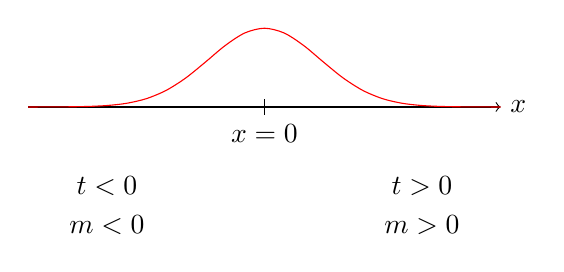
\begin{tikzpicture}
    \draw[->] (-3, 0) -- (3, 0) node[right]{$x$};
    \draw (0, -0.1) node[below]{$x = 0$} -- (0, 0.1);
    \draw (-2, -1) node[]{$\de t < 0$};
    \draw (-2, -1.5) node[]{$m < 0$};
    \draw (2, -1) node[]{$\de t > 0$};
    \draw (2, -1.5) node[]{$m > 0$};
    \draw[scale=1.0,domain=-3:3,smooth,variable=\x,red] plot ({\x},{exp(-\x*\x)});
\end{tikzpicture}
\end{center}

\subsection{Higher Dimensions}

A crystal is an infinite, periodic array of identical groups of atoms,
\[ \text{crystal} = \br{\text{basis}, \text{Bravais lattice}} \]

\begin{center}
    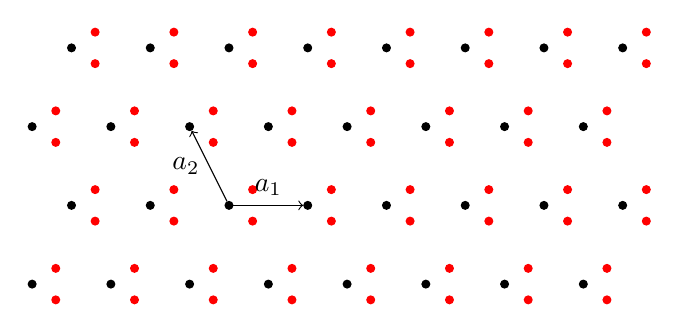
\begin{tikzpicture}
        \foreach \i in {1,...,8}
        {
            \foreach \j in {1,...,4}
            {
                \node[draw, fill, circle, inner sep=1pt] (\i\j) at ({\i+0.5*iseven(\j)},\j) {};
                \node[draw, fill, red, circle, inner sep=1pt] (a\i\j) at ({\i+0.5*iseven(\j)+0.3},\j-0.2) {};
                \node[draw, fill, red, circle, inner sep=1pt] (b\i\j) at ({\i+0.5*iseven(\j)+0.3},\j+0.2) {};
            }
        }
        \draw[->] (32) -- node[left]{$\ve a_2$} (33);
        \draw[->] (32) -- node[above]{$\ve a_1$} (42);
    \end{tikzpicture}
\end{center}

A \term{Bravais lattice} is all points in $\R^{n}$ ($\R^{1}, \R^{2}, \R^{3}$, etc.) such that,
\[ \ve R = n_1 \ve a_1 + n_2 \ve a_2 + n_3 \ve a_3 \eq \label{eq:R_lattice} \]
Where $\ve a_1, \ve a_2, \ve a_3$ are the primitive translation vectors of the Bravais lattice. Moreover the coefficients $n_1, n_2, n_3$ are integers,
\[ n_1, n_2, n_3 = 0, \pm 1, \pm 2, \pm 3, \ldots \]
Typically, the choice for $\ve a_i$ is not unique. However, the best choice for the primitive transition vectors is typically the one that exhibits the most symmetry. \\

The \term{primitive unit cell} is the parallelepiped defined by the primitive translation vectors. A primitive unit cell is also not unique. A special type of unit cell, usually the most convenient, is the \term{Wigner-Seitz unit cell}. A Wigner-Seitz unit cell is the region of space about a Bravais lattice point that are closer to this point than to any other Bravais lattice point. As an example, the first Brillouin zone is the Wigner-Seitz cell in reciprocal (momentum) space. Analogously to \cref{eq:R_lattice} which indexes lattice points in position space, we define the \term{reciprocal lattice} and all points in momentum space $\ve G$ such that,
\[ \ve G = m_1 \ve b_1 + m_2 \ve b_2 + m_3 \ve b_3\]
Provided that we have the following correspondence between $\ve R$ and $\ve G$,
\[ e^{i \ve G \cdot \ve P} = 1 \]
This is equivalent to the following,
\[ \ve b_{i} \cdot \ve a_{j} = 2 \pi \de_{ij} \qquad \forall i,j \]

\subsection{Electronic Structure for Square Lattice}

The square lattice in 2 dimensions has two primitive basis vectors $\ve a_{1}, \ve a_{2}$,
\begin{center}
    \begin{tikzpicture}
        \foreach \i in {1,...,8}
        {
            \foreach \j in {1,...,4}
            {
                \node[draw, fill, circle, inner sep=1pt] (\i\j) at (\i,\j) {};
            }
        }
        \draw[->] (32) -- node[left]{$\ve a_2$} (33);
        \draw[->] (32) -- node[above]{$\ve a_1$} (42);
    \end{tikzpicture}
\end{center}
Using Cartesian coordinates,
\[ \ve a_1 = a \hat x \qquad \ve a_2 = a \hat y \]
The reciprocal lattice has the following form,
\[ \ve b_1 = \f{2 \pi }{a}\hat x \qquad \ve b_2 = \f{2 \pi}{a} \hat y \]
The Hamiltonian for this system in the nearest neighbor approximation can be written as the sum over all possible transitions with tunneling coefficient $t$.
\[ H = - t \sum_{\ve R, \ve a} \br{\ket{\ve R + \ve a} \bra{\ve R} + \ket{\ve R} \bra{\ve R + \ve a}} \eq \label{eq:nearest_neighbor_square_lattice} \]
Where $\ve a \in \bc{\ve a_1, \ve a_2}$. Notice that we only need to sum over terms of the form involving $\ve R + \ve a$ and not $\ve R - \ve a$. If we were to include those terms, we would double-count all each of the possible transitions. In order to diagonalize \cref{eq:nearest_neighbor_square_lattice} we use the familiar Fourier transform but here we apply it as a vector change of coordinates,
\[\ket{\ve R} = \sum_{\ve R} \ket{\ve k} \braket{\ve k}{\ve R} \]
Where $\braket{\ve k}{\ve R}$ is normalized in the usual fashion,
\[ \braket{\ve k}{\ve R} = \f{1}{\sqrt{N}} e^{i \ve k \cdot \ve R} \]
Therefore,
\[\ket{\ve R} = \f{1}{\sqrt{N}} \sum_{\ve R} \ket{\ve k}  e^{i \ve k \cdot \ve R} \]
In the reciprocal lattice, $\ve k$ can be written as,
\[ \ve k = k_1 \ve b_1 + k_2 \ve b_2 \]
Where $k_{1}$ and $k_{2}$ are bounded,
\[ -\f12 \leq k_{1}, k_{2} < \f12 \]
Therefore,
\[ \ve k \cdot \ve R = \br{k_1 \ve b_1 + k_2 \ve b_2} \cdot \br{n_1 \ve a_1 + n_2 \ve a_2} \]
\[ \ve k \cdot \ve R = 2 \pi \br{k_1 n_1 + k_2 n_2} \]
Using the $\ket{\ve k}$ basis, \cref{eq:nearest_neighbor_square_lattice} becomes,
\[ H = - t \sum_{\ve R, \ve a} \sum_{\ve k, \ve k'} \br{\ket{\ve k}\bra{\ve k'} e^{-i \ve k \cdot \br{\ve R + \ve a}} e^{i \ve k' \cdot \ve R} + \ket{\ve k}\bra{\ve k'} e^{-i \ve k \cdot \ve R} e^{i \ve k' \cdot \br{\ve R + \ve a}}} \eq \label{eq:nearest_neighbor_square_lattice_momentum} \]
Using a multi-dimensional version of \cref{eq:crucial_idenity},
\[ \f{1}{N} \sum_{\ve R} e^{- i \br{\ve k - \ve k'} \cdot \ve R} = \de_{\ve k, \ve k'} \]
Therefore \cref{eq:nearest_neighbor_square_lattice} becomes,
\[ H = - t \sum_{\ve k, \ve a} \ket{\ve k} \bra{\ve k} \br{e^{- i\ve k \cdot \ve a} + e^{i\ve k \cdot \ve a}} \]
Recognize a cosine term,
\[ H = - 2t \sum_{\ve k, \ve a} \ket{\ve k} \bra{\ve k} \cos \br{\ve k \cdot \ve a} \]
The energy levels (as indexed by $\ve k$) can now be read off easily,
\[ \vep \br{\ve k} = -2 t \sum_{\ve a} \cos \br{\ve k \cdot \ve a} = - 2t \bs{ \cos \br{ ak_x} + \cos \br{ ak_y}} \]
Clearly, $\vep\br{\ve k}$ has minimum when $k_x = k_y = 0$. Therefore,
\[ \min\bc{\vep\br{\ve k}} = \vep_{\min} = - 4 t \]
Likewise at the Brillouin zone corners,
\[ \max\bc{\vep\br{\ve k}} = \vep_{\max} = 4 t \]
\begin{center}
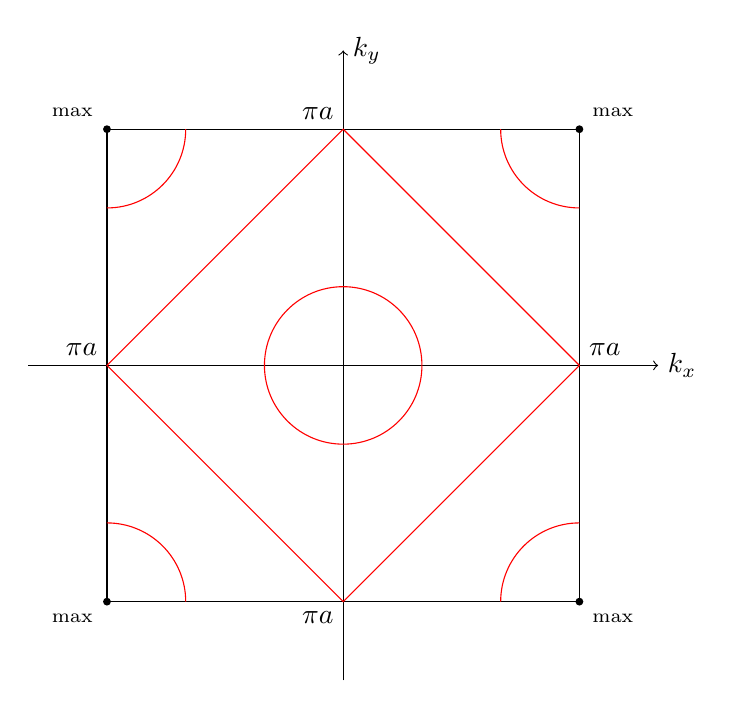
\begin{tikzpicture}
    \pgfmathsetmacro{\plot}{4};
    \pgfmathsetmacro{\edge}{3};
    \pgfmathsetmacro{\oarc}{1};
    \draw[->] (-\plot, 0) -- (\plot, 0) node[right]{$k_x$};
    \draw[->] (0, -\plot) -- (0, \plot) node[right]{$k_y$};
    \draw (+\edge, +\edge) -- (+\edge, -\edge);
    \draw (+\edge, -\edge) -- (-\edge, -\edge);
    \draw (-\edge, +\edge) -- (+\edge, +\edge);
    \draw (-\edge, -\edge) -- (-\edge, +\edge);
    \draw (+\edge, 0) node[above right]{$\f{\pi}{a}$};
    \draw (0, +\edge) node[above left]{$\f{\pi}{a}$};
    \draw (-\edge, 0) node[above left]{$\f{\pi}{a}$};
    \draw (0, -\edge) node[below left]{$\f{\pi}{a}$};
    \draw (+\edge, +\edge) node[circle, inner sep=1pt, fill=black, label={above right:$\vep_{\max}$}]{};
    \draw (-\edge, +\edge) node[circle, inner sep=1pt, fill=black, label={above left:$\vep_{\max}$}]{};
    \draw (+\edge, -\edge) node[circle, inner sep=1pt, fill=black, label={below right:$\vep_{\max}$}]{};
    \draw (-\edge, -\edge) node[circle, inner sep=1pt, fill=black, label={below left:$\vep_{\max}$}]{};
    \draw[red] (+\edge, 0) -- (0, +\edge) -- (-\edge, 0) -- (0, -\edge) -- cycle;
    \draw[red] (0,0) circle (\edge/3);
    \draw[red] (+\edge-\oarc, +\edge) arc (180:270:\oarc);
    \draw[red] (-\edge, +\edge-\oarc) arc (270:360:\oarc);
    \draw[red] (+\edge-\oarc, -\edge) arc (180:90:\oarc);
    \draw[red] (-\edge, -\edge+\oarc) arc (90:0:\oarc);
\end{tikzpicture}
\end{center}
Expanding $\ve k$ near the minimum,
\[ \vep\br{\ve k} \simeq -4t + t a^2 \br{k_x^2 + k_y^2} = -4t + ta^2 k^2 \eq \label{eq:minimum_k}\]
Notice that this looks like the dispersion of a free electron.
Recall that for a free electron,
\[ \vep \br{\ve k} = \f{\hbar^2 k^2}{2 m} \]
Therefore we can define an effective mass $m^{*}$ as follows,
\[ \vep \br{\ve k} - \vep_{\min} = ta^2 k^2 = \f{\hbar^2 k^2}{2 m^{*}} \]
Where the effective mass is,
\[ m^{*} = \f{\hbar^2}{2 t a^2} \]
In conclusion, electrons near the minimum energy level $\vep_{\min}$ behave like free particles with effective mass $m^{*}$. \\

The Fermi surface in this model can be calculated by setting $\vep \br{\ve k} = \vep\tsb{F}$,
\[ \vep\br{\ve k} = - 4t + \f{\hbar^2 k^2}{2 m^{*}} = \vep\tsb{F}\]
Therefore,
\[ \f{\hbar^2 k^2}{2 m^{*}} = \vep\tsb{F} - \vep_{\min} \]
Defines the equation of a circle in $k_x, k_y$ space with radius,
\[ k_{F} = \sqrt{\f{2m^{*}}{\hbar^2} \br{\vep\tsb{F} - \vep_{\min}}} \]
Recall from \cref{eq:minimum_k} that this equation only defines the Fermi surface near the minimum energy level. In general,
\[ \vep \br{\ve k} = - 2t \br{\cos \br{k_x a} + \cos \br{k_y a}} \]
For a half-filled band, $\vep\tsb{F} = 0$, the Fermi surface is depicted above.

The dispersion relation is,
\begin{center}
    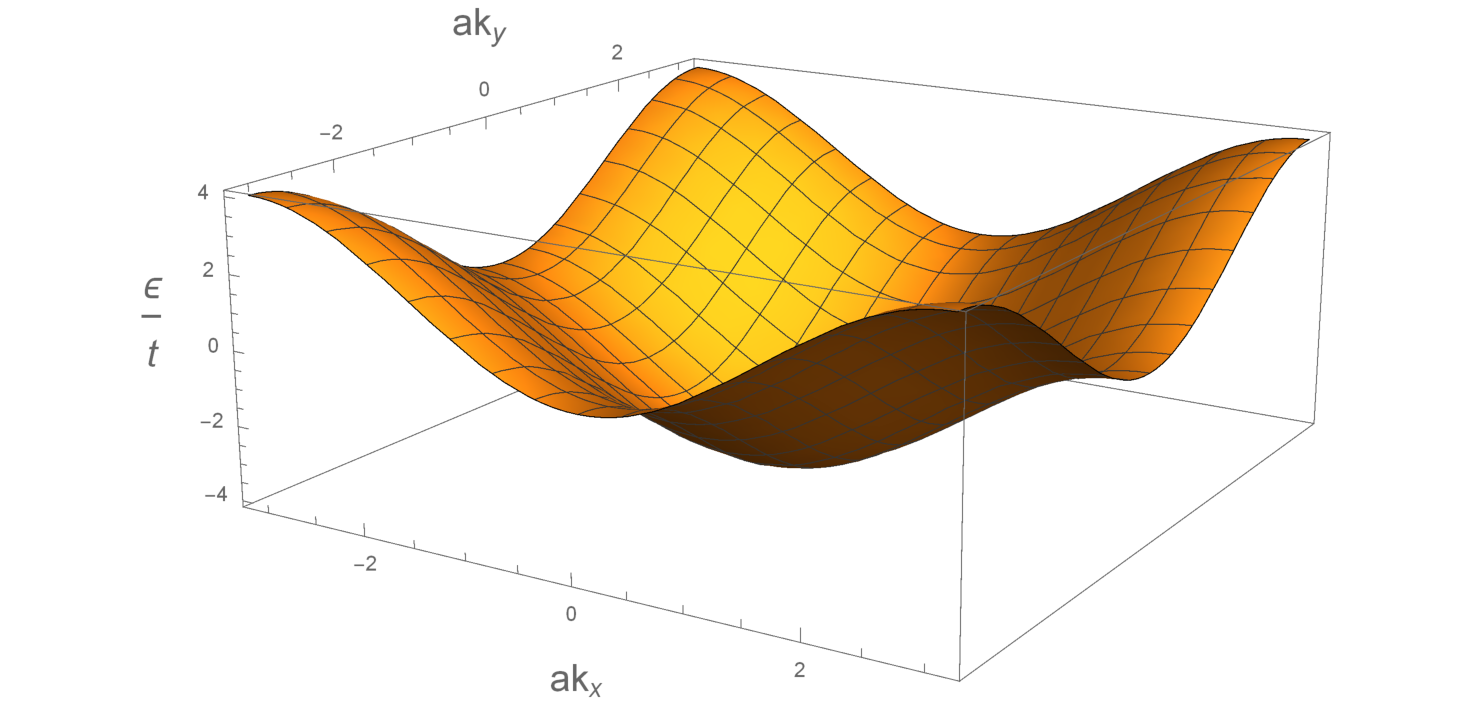
\includegraphics[width=0.9\textwidth]{figures/square_3d_bz.pdf}
    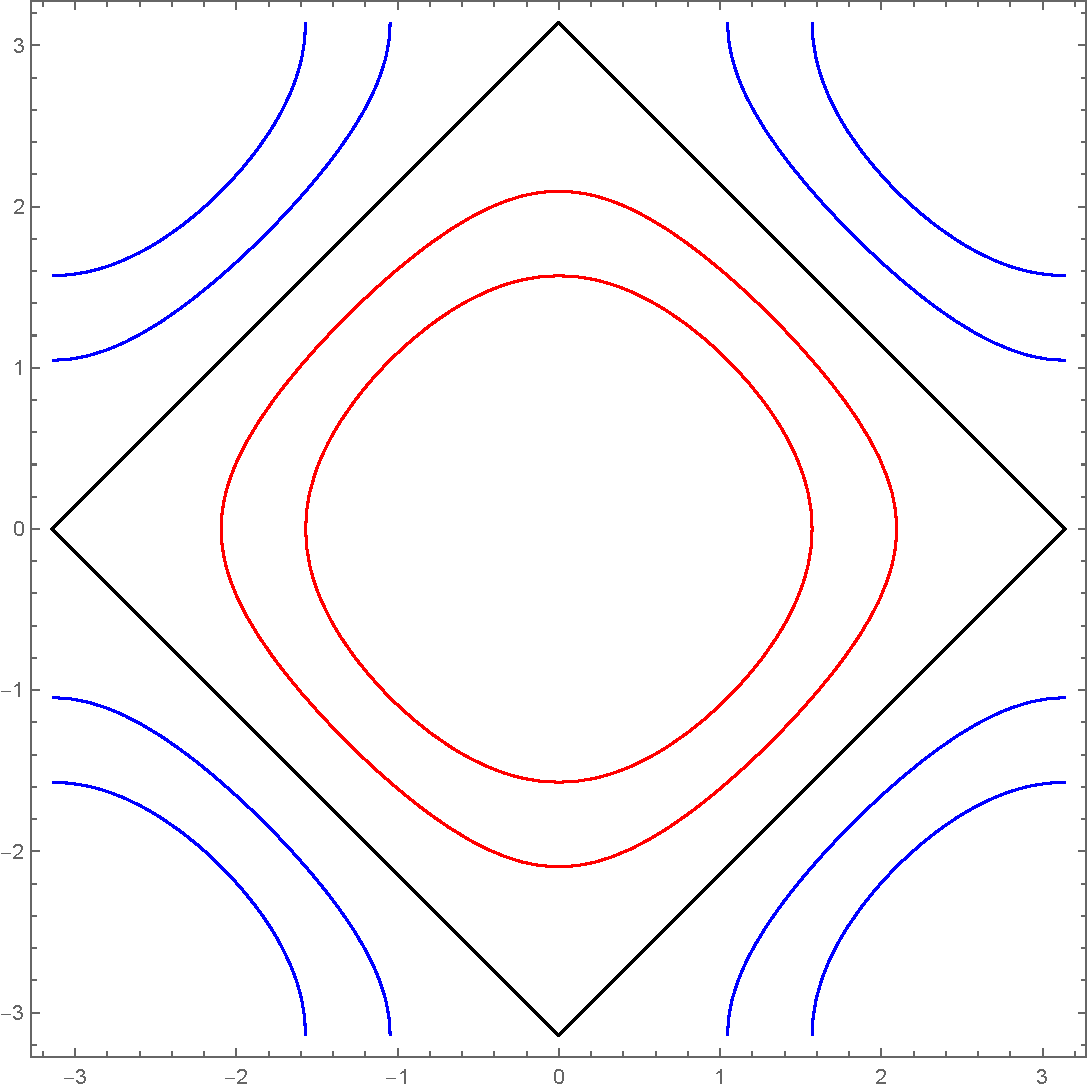
\includegraphics[width=0.6\textwidth]{figures/square_3d_bz_fermi_surface.pdf}
\end{center}

\subsection{Graphene}

The primitive unit vectors for Graphene are,
\[ \ve a_{1} = \f{a}{2} \br{\hat x + \sqrt{3} \hat y} \qquad \ve a_{2} = \f{a}{2} \br{-\hat x + \sqrt{3} \hat y} \eq \label{eq:gp_graphen_a} \]
Where the lattice structure is as follows,
\begin{center}
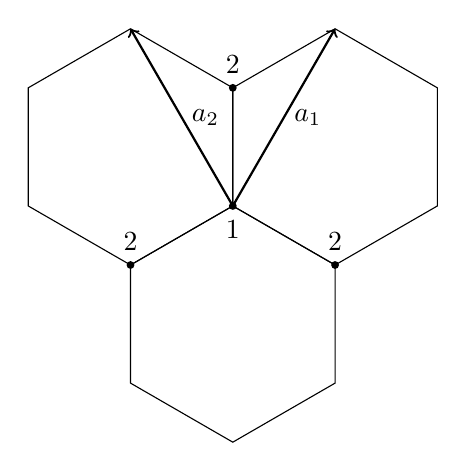
\begin{tikzpicture}
    \pgfmathsetmacro{\size}{1.5};
    \pgfmathsetmacro{\f}{sqrt(3)/2};
    \pgfmathsetmacro{\ss}{1/2};
    \draw (0,0) node[circle, inner sep=1pt, fill=black, label={below:$1$}]{};
    \draw (0,\size) node[circle, inner sep=1pt, fill=black, label={above:$2$}]{};
    \draw (\f*\size,-\ss*\size) node[circle, inner sep=1pt, fill=black, label={above:$2$}]{};
    \draw (-\f*\size,-\ss*\size) node[circle, inner sep=1pt, fill=black, label={above:$2$}]{};
    \draw (0,0) -- ++(\f*\size,-\ss*\size) -- ++(\f*\size,\ss*\size) -- ++(0, \size) -- ++(-\f*\size,\ss*\size) -- ++(-\f*\size,-\ss*\size) -- cycle;
    \draw (0,0) -- ++(0, \size) -- ++(-\f*\size,\ss*\size) -- ++(-\f*\size,-\ss*\size) --++(0, -\size) -- ++(\f*\size,-\ss*\size) -- ++(\f*\size,\ss*\size) -- cycle;
    \draw (0,0)  -- ++(-\f*\size,-\ss*\size) --++(0, -\size) -- ++(\f*\size,-\ss*\size) -- ++(\f*\size,\ss*\size) -- ++(0, \size) -- cycle;
    \draw[thick, ->] (0,0) -- node[right]{$\ve a_1$} ++(0+\f*\size, \size+\ss*\size);
    \draw[thick, ->] (0,0) -- node[right]{$\ve a_2$} ++(0-\f*\size, \size+\ss*\size);
\end{tikzpicture}
\end{center}

\[ \ve b_{1} = \f{2 \pi}{a} \br{\hat x + \sqrt{3} \hat y} \qquad \ve b_{2} = \f{2 \pi}{a} \br{-\hat x + \sqrt{3} \hat y} \eq \label{eq:gp_graphen_b}\]
The nearest neighbor Hamiltonian becomes,
\[ H = -t \sum_{\ve R} \br{\ket{\ve R, 2} \bra{\ve R, 1} + \ket{\ve R - \ve a_{1}, 2}\bra{\ve R, 1} + \ket{\ve R - \ve a_2, 2}\bra{\ve R, 1} + \text{h.c.}}\eq \label{eq:gp_graphene_H_nn} \]
In the reciprocal lattice,
\[ \ket{\ve R, \al} = \f{1}{\sqrt{N}} \sum_{\ve R} \ket{\ve k, \al} e^{-i \ve k \cdot \ve R} \]
Therefore the Hamiltonian becomes,
\begin{align*}
    H
    &= -\f{t}{N} \sum_{\ve R}\sum_{\ve K, \ve K'} \Bigg( \ket{\ve k, 2}\bra{\ve k,1}e^{-i \ve k \cdot \ve R} e^{i \ve k' \cdot \ve R} + \ket{\ve k, 2}\bra{\ve k,1}e^{-i \ve k \cdot \br{\ve R - \ve a_1}} e^{i \ve k' \cdot \ve R}+ \ket{\ve k, 2}\bra{\ve k,1}e^{-i \ve k \cdot \br{\ve R - \ve a_2}} e^{i \ve k' \cdot \ve R} + \text{h.c.} \Bigg) \\
\end{align*}
\[ H = - t\sum_{\ve k}\bs{\ket{\ve k, 2} \bra{\ve k, 1} \br{1 + e^{i \ve k \cdot \ve a_1} + e^{i \ve k \cdot \ve a_2}} + \ket{\ve k, 1} \bra{\ve k, 2} \br{1 + e^{-i \ve k \cdot \ve a_1} + e^{-i \ve k \cdot \ve a_2}}} \]
We have now diagonalized $H$ in terms of the momentum wave-vector index $\ve k$. Letting $H = \sum_{\ve k} H\br{\ve k}$ where,
\[ H\br{\ve k} = -t\bs{\ket{ 2} \bra{ 1} \br{1 + e^{i \ve k \cdot \ve a_1} + e^{i \ve k \cdot \ve a_2}} + \ket{ 1} \bra{ 2} \br{1 + e^{-i \ve k \cdot \ve a_1} + e^{-i \ve k \cdot \ve a_2}}} \]
Invoking pseudo-spin states $\ket{1} = \ket{\uparrow}$ and $\ket{2} = \ket{\downarrow}$ we can write,
\[ H\br{\ve k} = \ve d\br{\ve k} \cdot \ve \si \]
Where $\ve d \br{\ve k}$ is,
\begin{align*}
    d^{x}\br{\ve k} & = -t \bs{1 + \cos\br{\ve k \cdot \ve a_1} + \cos \br{\ve k \cdot \ve a_2}} \\
    d^{y}\br{\ve k} & = -t \bs{\sin\br{\ve k \cdot \ve a_1} + \sin \br{\ve k \cdot \ve a_2}} \\
    d^{z}\br{\ve k} & = 0
\end{align*}
The eigenvalues of $H\br{\ve k}$ are then the usual,
\[ \vep_{\pm}\br{\ve k} = \pm \abs{\ve d\br{\ve k}} \]
Since we have $1$ electron per carbon atom, there are 2 electrons per unit cell which means that the $\vep_{-}$ band is completely filled while the $\vep_{+}$ is empty. For this configuration, the conduction band is empty and thus graphene is an insulator. \\

In order to analyze the electronic structure of graphene, we need to rewrite $\ve k$ which is expressed via the reciprocal lattice vectors $\ve b_1, \ve b_2$ in terms of the Cartesian vectors $\ve a_1, \ve a_2$.
\[ \ve k = k_1 \ve b_1 + k_2 \ve b_2 \]
\[ \ve k \cdot \ve a_1 = \br{k_1 \ve b_1 + k_2 \ve b_2} \cdot \ve a_1 = 2 \pi k_1 \qquad \ve k \cdot \ve a_2 = 2 \pi k_2 \]
Recalling \cref{eq:gp_graphen_a,eq:gp_graphen_b},
\[ \ve a_{1} = \f{a}{2} \br{\hat x + \sqrt{3} \hat y} \qquad \ve a_{2} = \f{a}{2} \br{-\hat x + \sqrt{3} \hat y} \]
\[ \ve b_{1} = \f{2 \pi}{a} \br{\hat x + \sqrt{3} \hat y} \qquad \ve b_{2} = \f{2 \pi}{a} \br{-\hat x + \sqrt{3} \hat y}\]
We can now write $k_x, k_y$ in terms of $k_1, k_2$,
\[ k_x = \f{2 \pi }{\sqrt{3}a} \br{k_1 - k_2} \qquad k_y = \f{2 \pi}{\sqrt{3}a} \br{k_1 + k_2} \]
Inverting this system gives,
\[ k_1 = \f{a}{4 \pi} \br{k_x + \sqrt{3} k_y} \qquad k_2 = \f{a}{4 \pi} \br{-k_x + \sqrt{3} k_y} \]
Therefore,
\begin{align*}
    d^{x}\br{\ve k}
    &= - t\bs{1 + \cos\br{2 \pi k_1} + \cos\br{2 \pi k_2}} \\
    &= - t\bs{1 + 2\cos\br{\f{k_xa}{2}}\cos\br{\f{\sqrt{3}k_ya}{2}}}
\end{align*}
Similarly for $d^{y}\br{\ve k}$,
\[ d^{y}\br{\ve k} = -2 t \cos\br{\f{k_x a}{2}} \sin\br{\f{\sqrt{3} k_y a}{2}} \]
By examining these equations it can be seen that there are two points (and only two points) in the first Brillouin zone where both $d^{x}$ and $d^y$ vanish simultaneously. We label these points as $\ve k_{\pm}$,
\[ \ve k_+ = \br{k_{+, x}, k_{+, y}} = \br{\f{4 \pi }{3a}, 0} \]
\[ \ve k_- = \br{k_{-, x}, k_{-, y}} = \br{-\f{4 \pi }{3a}, 0} \]
At either of these points,
\[ \abs{\ve d \br{\ve k_{\pm}}} = \sqrt{{d^x}^2\br{\ve k} + {d^y}^2\br{\ve k}} = 0 \]
Therefore, the gap between the $\vep_{+}$ band and the $\vep_{-}$ closes at only two points. Since graphene is an insulator and does not have a Fermi surface (meaning its \textit{not} a metal) we refer to graphene, and materials that share these features, as \term{semimetals}. \\


The Brillouin zone of graphene can be derived using \cref{eq:gp_discrete_k} and \cref{eq:gp_kxky}. First, rewrite $\ve k$ which is typically defined in terms of the reciprocal lattice vectors $\ve b_1, \ve b_2$ in terms of the Cartesian vectors $\ve a_1, \ve a_2$.
\[ \ve k = k_1 \ve b_1 + k_2 \ve b_2 \qquad \ve b_i \cdot \ve a_j = 2 \pi \de_{ij}\]
\[ \ve k \cdot \ve a_1 = \br{k_1 \ve b_1 + k_2 \ve b_2} \cdot \ve a_1 = 2 \pi k_1 \qquad \ve k \cdot \ve a_2 = 2 \pi k_2 \]
Therefore using \cref{eq:gp_kxky} yields,

\begin{align*}
\eq \label{eq:gp_k1k2}
\begin{split}
k_1 &= \f{a}{4 \pi}\br{k_x + \sqrt{3}k_y} \\
k_2 &= \f{a}{4 \pi}\br{-k_x + \sqrt{3}k_y}
\end{split}
\end{align*}
Recalling \cref{eq:gp_graphene_a},
\[ \ve a_{1} = \f{a}{2} \br{\hat x + \sqrt{3} \hat y} \qquad \ve a_{2} = \f{a}{2} \br{-\hat x + \sqrt{3} \hat y} \]
\[ \ve b_{1} = \f{2 \pi}{a\sqrt{3}} \br{\sqrt{3} \hat x +  \hat y} \qquad \ve b_{2} = \f{2 \pi}{a\sqrt{3}} \br{-\sqrt{3}\hat x +  \hat y}\]
We can now write $k_x, k_y$ in terms of $k_1, k_2$,
\[ k_x = \f{2 \pi }{a} \br{k_1 - k_2} \qquad k_y = \f{2 \pi}{\sqrt{3}a} \br{k_1 + k_2} \]
Using \cref{eq:gp_periodic_boundary},
\[ 1 = e^{i N_i \ve k \cdot \ve a_i} \implies N_i \ve k \cdot \ve a_i = N_i 2 \pi k_i = 2 \pi m_i \implies N_i k_i = m_i \]
% \[ \abs{\ve b}^2 \leq 4\f{\br{2 \pi}^2}{a^2} \]
% \[ -2\f{\br{2 \pi}}{a} \leq \abs{\ve b} \leq 2\f{\br{2 \pi}}{a} \]
% Therefore,
% \[ 2N_i k_i = m_i \in \Z \]
Where $m_i \in \Z$ is an integer and $i \in \bc{1,2}$.\\

Moreover, since there are $N_i$ unit cells in the $\ve a_i$ direction we have,
\[ - \f{N_i}{2} \leq m_i < \f{N_i}{2} \qquad m_i \in \Z, \forall i \in \bc{1,2} \]
Therefore,
\[ - \f{N_i}{2} \leq N_i k_i < \f{N_i}{2} \qquad \forall i \in \bc{1,2} \]
\[ - \f{1}{2} \leq k_i < \f{1}{2} \qquad \forall i \in \bc{1,2} \]
This result is intuitive. The first Brillouin zone only extends halfway in the direction of $\ve b_1, \ve b_2$ or combinations thereof. These inequalities yield the following,
\[ \abs{k_1}, \abs{k_2} < \f12  \]
\[ \ve k = k_x \hat x + k_y \hat y  \]
Where the norms of $\ve b_i$ are independent of $i$.
\[ b^2 = \abs{\ve b_1}^2 = \abs{\ve b_2}^2 =  4\f{\br{2 \pi}^2}{3a^2} = \f{16 \pi^2}{3a^2}\]
\[ \f12 \leq \f{\ve k \cdot \ve b_i}{b^2} = k_i \leq \f12  \]
Therefore,
\[ -\f12 \leq \f{1}{b^2} \br{\f{2 \pi}{a\sqrt{3}} \br{\sqrt{3} \hat x +  \hat y}} \cdot \br{k_x \hat x + k_y \hat y} \leq \f12  \]
\[ -\f12 \leq \f{3a^2}{4\br{2 \pi}^2} \br{\f{2 \pi}{a\sqrt{3}} \br{\sqrt{3} k_x +  k_y}} \leq \f12  \]
\[ -\f{4}{\sqrt{3}}\pi \leq  a\br{\sqrt{3} k_x +  k_y} \leq \f{4}{\sqrt{3}}\pi  \]
Similarly,
\[ -\f{4}{\sqrt{3}}\pi \leq  a\br{-\sqrt{3} k_x +  k_y} \leq \f{4}{\sqrt{3}}\pi  \]
And the positive sum of these two inequalities gives,
\[ -\f{4}{\sqrt{3}}\pi \leq  ak_y \leq \f{4}{\sqrt{3}}\pi  \]
Which does not constrain the first Brillouin zone any further. Instead we invoke,
\[ \f12 \leq \f{\ve k \cdot \br{\ve b_1 + \ve b_2}}{b^2} \leq \f12  \]
Which becomes,
\[ -\f{4}{\sqrt{3}}\pi \leq 2ak_y \leq \f{4}{\sqrt{3}}\pi  \]
Therefore the Brillouin zone is fully characterized.
\begin{center}
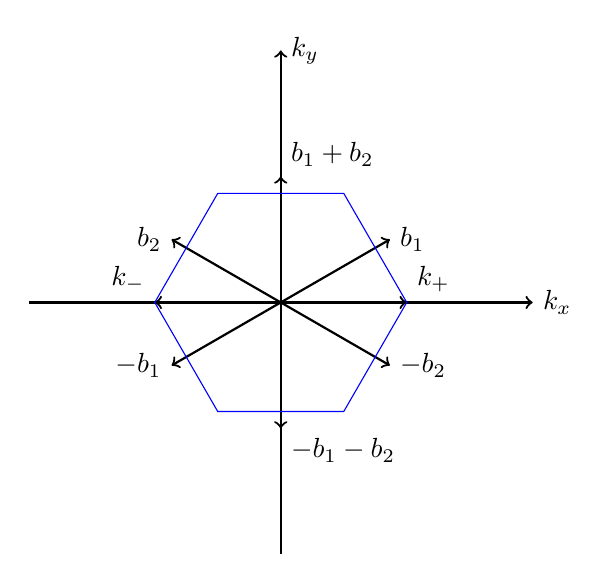
\begin{tikzpicture}[scale=0.8]
    \pgfmathsetmacro{\plot}{4};
    \pgfmathsetmacro{\st}{sqrt(3)};
    \pgfmathsetmacro{\size}{3};
    \draw[thick,->] (-\plot, 0) -- (\plot, 0) node[right]{$k_x$};
    \draw[thick,->] (0, -\plot) -- (0, \plot) node[right]{$k_y$};
    \draw[thick,->] (0,0) -- (\st, 1)         node[right]{$\ve b_1$};
    \draw[thick,->] (0,0) -- (-\st, 1)        node[left]{$\ve b_2$};
    \draw[thick,->] (0,0) -- (\st, -1)        node[right]{$-\ve b_2$};
    \draw[thick,->] (0,0) -- (-\st, -1)       node[left]{$-\ve b_1$};
    \draw[thick,->] (0,0) -- (0, -2)          node[below right]{$-\ve b_1 -\ve b_2$};
    \draw[thick,->] (0,0) -- (0, 2)           node[above right]{$\ve b_1 +\ve b_2$};
    \draw[thick,->] (0,0) -- (2/3*\size, 0)   node[above right]{$\ve k_+$};
    \draw[thick,->] (0,0) -- (-2/3*\size, 0)  node[above left]{$\ve k_-$};
    \draw[blue]
    (2/3*\size, 0) --
    (1, \st)       --
    % (0, 2*\st)     --
    (-1, \st)      --
    (-2/3*\size, 0)--
    % (0, -2*\st)    --
    (-1, -\st)     --
    (1, -\st)      --
    cycle;
\end{tikzpicture}
\end{center}
\begin{center}
    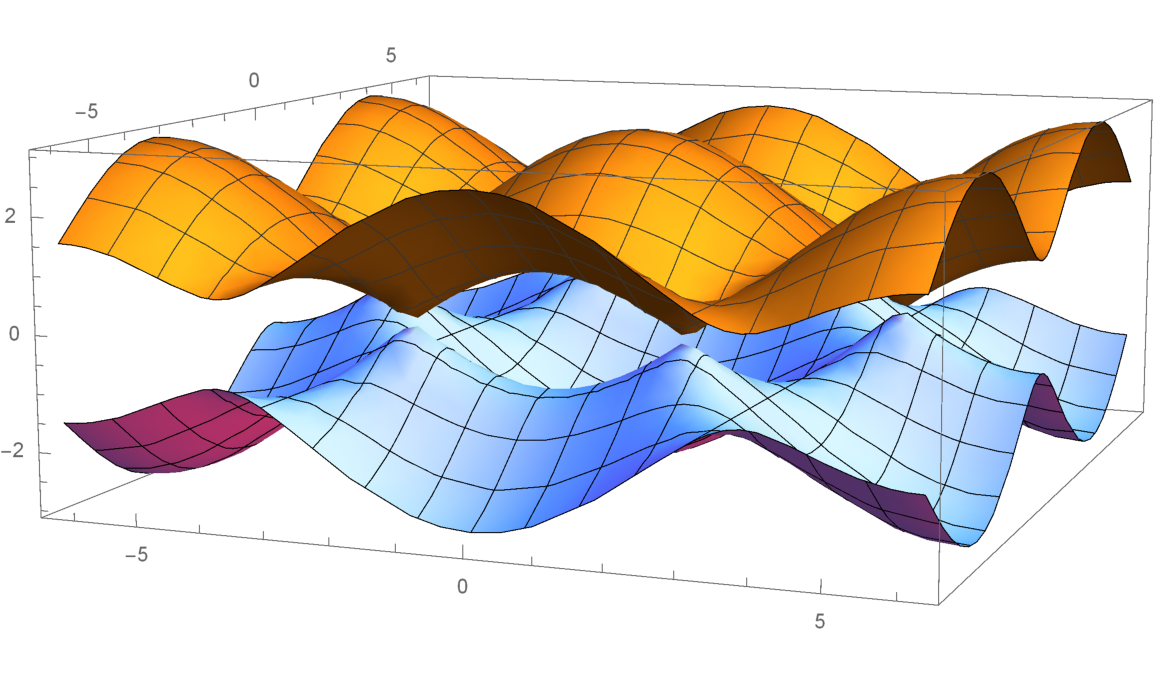
\includegraphics[width=0.45\linewidth]{figures/graphene_3d_dr.pdf}
    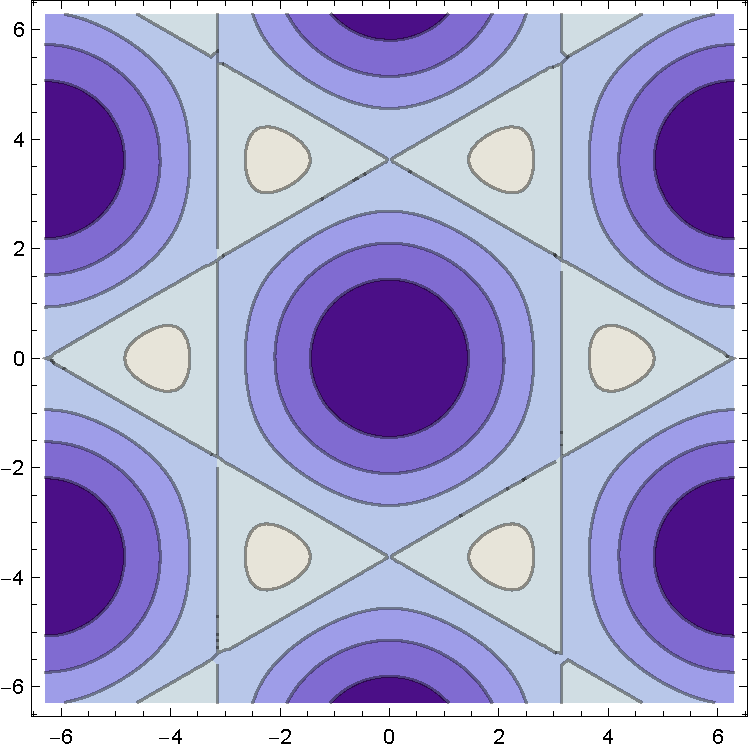
\includegraphics[width=0.25\linewidth]{figures/graphene_3d_contour_dr.pdf}
    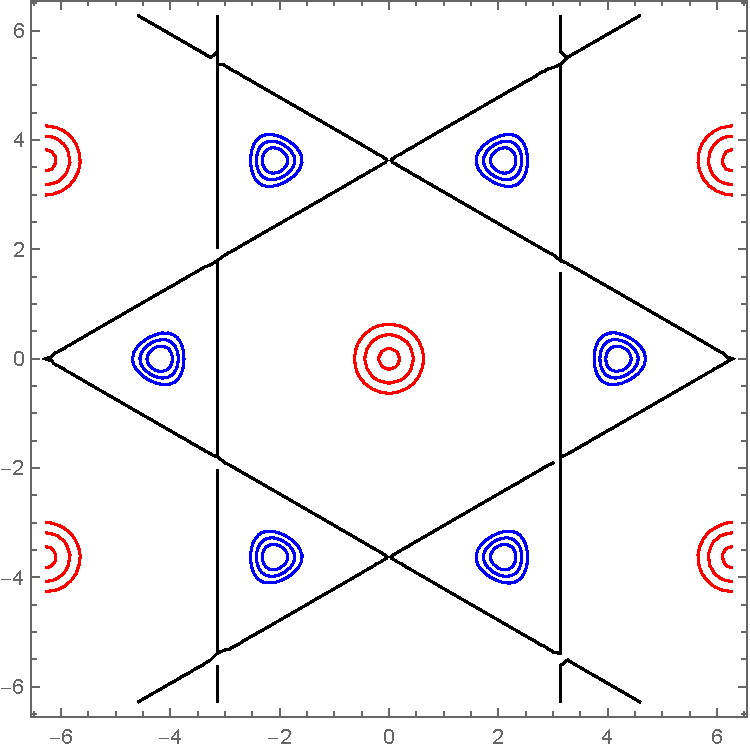
\includegraphics[width=0.25\linewidth]{figures/graphene_3d_contour_bz.pdf}
\end{center}
The first Brillouin zone for graphene forms a hexagonal lattice with the corners obtained from $\ve k_{\pm}$ by adding $\pm b_1, \pm b_2$,
\[ \ve G = m_1 \ve b_2 + m_2 \ve b_2 \]
In graphene, the upper and lower band are \textit{not} separated by a band gap (sometimes $\vep_{+} > \vep_{-}$ and sometimes $\vep_{+} < \vep_{-}$). The crossing points are precisely the two points where $\ve k = \ve k_{\pm}$. If we expand $H\br{\ve k}$ near $\ve k_{\pm}$ to first order,
\[ k_x = k_{x, \pm} + \de k_x  \qquad k_y = \de k_y\]
To first order,
\[ d^{x}_{\pm} \br{\de \ve k} \simeq \pm \f{\sqrt{3}}{2} t a \de k_x \]
\[ d^{y}_{\pm} \br{\de \ve k} \simeq \f{\sqrt{3}}{2} t a \de k_y \]
For both the $x$ and $y$ directions, the leading coefficient $\f{\sqrt{3}}{2} t a$ has units of speed times $\hbar$. We again call this the Fermi velocity,
\[ v\tsb{F} = \f{\sqrt{3} t a}{2\hbar} \]
Then we can write the Hamiltonian as,
\[ H_{\pm}\br{\ve k} = \hbar v\tsb{F} \br{\pm k_x \si^x + k_y \si^{y}} \eq \label{eq:gp_2d_dirac}\]
Where here $k_x$ and $k_y$ refer to $\de k_x$ and $\de k_y$. This is done by shifting coordinates such that $\ve k_{\pm} = 0$ for each of the $+, -$ cases. Upon examination of \cref{eq:gp_2d_dirac}, \cref{eq:gp_2d_dirac} takes the form of a 2D Dirac Hamiltonian for a massless relativistic particle in 2D. The energies near the touching points $\ve k_{\pm}$ is,
\[ \vep\br{\ve k} = \pm \hbar v\tsb{F} k \]
Where $k = \sqrt{k_x^2 + k_y^2}$. This means that $\vep\br{\ve k}$ has linear dispersion near $\ve k_{\pm}$. \\

One question we can ask is what can we do to graphene in order to open a gap between $\ve k_{-}$ and $\ve k_{+}$. In order words, how can we give the electron in \cref{eq:gp_2d_dirac} an effective mass. This can be accomplished by introducing a discrepancy between the atoms labeled $1$ and the atoms labeled $2$ within a unit cell. As an example, we can add energies $\pm m$ to the atoms as follows,

\begin{center}
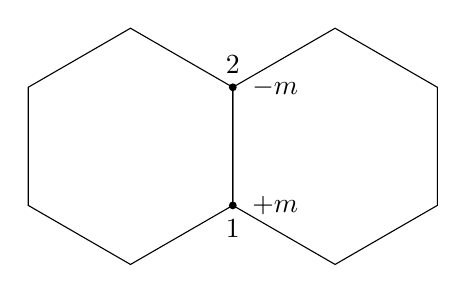
\begin{tikzpicture}
    \pgfmathsetmacro{\size}{1.5};
    \pgfmathsetmacro{\f}{sqrt(3)/2};
    \pgfmathsetmacro{\ss}{1/2};
    \draw (0,0) node[circle, inner sep=1pt, fill=black, label={below:$1$}]{};
    \draw (0,\size) node[circle, inner sep=1pt, fill=black, label={above:$2$}]{};
    \draw (0,\size) node[label={right:$-m$}]{};
    \draw (0,0) node[label={right:$+m$}]{};
    % \draw (\f*\size,-\ss*\size) node[circle, inner sep=1pt, fill=black, label={above:$2$}]{};
    % \draw (-\f*\size,-\ss*\size) node[circle, inner sep=1pt, fill=black, label={above:$2$}]{};
    \draw (0,0) -- ++(\f*\size,-\ss*\size) -- ++(\f*\size,\ss*\size) -- ++(0, \size) -- ++(-\f*\size,\ss*\size) -- ++(-\f*\size,-\ss*\size) -- cycle;
    \draw (0,0) -- ++(0, \size) -- ++(-\f*\size,\ss*\size) -- ++(-\f*\size,-\ss*\size) --++(0, -\size) -- ++(\f*\size,-\ss*\size) -- ++(\f*\size,\ss*\size) -- cycle;
    % \draw (0,0)  -- ++(-\f*\size,-\ss*\size) --++(0, -\size) -- ++(\f*\size,-\ss*\size) -- ++(\f*\size,\ss*\size) -- ++(0, \size) -- cycle;
    % \draw[thick, ->] (0,0) -- node[right]{$\ve a_1$} ++(0+\f*\size, \size+\ss*\size);
    % \draw[thick, ->] (0,0) -- node[right]{$\ve a_2$} ++(0-\f*\size, \size+\ss*\size);
\end{tikzpicture}
\end{center}

Which effectively corresponds to adding the following term to the original Hamiltonian,
\[ H' = m \sum_{\ve R} \br{\ket{\ve R, 1}\bra{\ve R, 1} - \ket{\ve R, 2}\bra{\ve R, 2}} \]


Applying the Fourier transform yields the following,
\[ H' = m \sum_{\ve k} \br{\ket{\ve k, 1}\bra{\ve k, 1} - \ket{\ve k, 2}\bra{\ve k, 2}} \]
Which further adjusts the dispersion relationship,
\[ H'\br{\ve k} = m \br{\ket{1}\bra{1} - \ket{2}\bra{2}} = m \si^{z} \]
Therefore,
\[ H_{\pm}\br{\ve k} =\hbar v\tsb{F} \br{\pm k_x \si^x + k_y \si^{y}} + m\si^{z} \]
\[ \vep_{\pm} \br{\ve k} = \pm \sqrt{\hbar^2 v\tsb{F} k^2 + m^2} \]
This opens up a band gap of size $2m$. Therefore clean graphene ($m=0$) is a semimetal due to inversion symmetry but becomes an insulator for $m > 0$. \\

Returning to the case of $m=0$,
\[ H_{\pm}\br{\ve k} =\hbar v\tsb{F} \br{\pm k_x \si^x + k_y \si^{y}} \]
The `$\pm$' can be thought of as a two component degree of freedom. Because there are two components, we can think of `$\pm$' as another pseudo-spin value $\tau$.
\begin{align*}
    \tau^{z} &= \ket{+} \bra{+} - \ket{-}\bra{-} \\
    \tau^{y} &= -i\br{\ket{+} \bra{-} - \ket{-}\bra{+}} \\
    \tau^{x} &= \ket{+} \bra{-} + \ket{-}\bra{+}
\end{align*}
Which means that the Hamiltonian can be written without the `$\pm$' as a single matrix,
\[ H\br{\ve k} =\hbar v\tsb{F} \br{k_x \tau^{z} \si^x + k_y \si^{y}} \eq \label{eq:gp_double2spin}\]

\subsubsection{Spin-Orbit Interactions}
\label{sec:soi}
What are the symmetries of \cref{eq:gp_double2spin}? We must have the following:
\begin{enumerate}
    \item Time Reversal Symmetry
    \item Inversion Symmetry
\end{enumerate}
In order to facilitate discussions, we introduce two operators; the \term{inversion (parity) operator $\pi$} and \term{time-reversal operator $\Theta$}. The symmetries of \cref{eq:gp_double2spin} can we written,
\[  \pi^{\dagger} H\br{\ve k} \pi = H\br{\ve k} \eq \label{eq:gp_parity_graphene}\]
\[  \Theta H\br{\ve k} \Theta^{-1} = H\br{\ve k} \eq \label{eq:gp_tr_graphene}\]
Since $\tau^{z}$ refers to the two band touching points (coordinates in momentum space), $\tau^{z}$ changes sign under both symmetries,
\[ \pi^{\dagger} \tau^{z} \pi = - \tau^{z} \eq \label{eq:gp_tau_z_sym_parity}\]
\[ \Theta \tau^{z} \Theta^{-1} = - \tau^{z} \eq \label{eq:gp_tau_z_sym_tr}\]
Furthermore, $k_{x, y, z}$ represent momentum and is thus time and parity odd,
\[ \pi^{\dagger} k_{x,y,z} \pi = - k_{x,y,z} \]
\[ \Theta k_{x,y,z} \Theta^{-1} = - k_{x,y,z} \]
Therefore we must conclude that $\si^{x}$ is even under these symmetries and $\si^{y}$ is odd pursuant to \cref{eq:gp_parity_graphene,eq:gp_tr_graphene},
\[ \pi^{\dagger} \si^{y} \pi = - \si^{y} \]
\[ \Theta \si^{y} \Theta^{-1} = - \si^{y} \]
\[ \pi^{\dagger} \si^{x} \pi = + \si^{x} \]
\[ \Theta \si^{x} \Theta^{-1} = + \si^{x} \]
This is intuitive because $\si$ refers to the spatial location of atoms $1$ and $2$ oriented in the $y$ direction.
If we were to include the massive term $m\si^{z}$ we break symmetry in \cref{eq:gp_parity_graphene,eq:gp_tr_graphene},
\[ \pi^{\dagger} \si^{z} \pi = - \si^{z} \qquad \Theta \si^{z} \Theta^{-1} = \si^{z} \eq \label{eq:gp_si_z_sym}\]
Specifically, $m \si^{z}$ breaks inversion symmetry. This is intuitive because $m$ adds spatial discrepancies between $1$ and $2$. Can we open a gap in graphene without breaking time-reversal or inversion symmetries?\\

Interestingly, this lack of symmetry is an artifact of the simplistic model introduced by \cref{eq:gp_graphene_H_nn}. If we include \textit{next-nearest neighbor} terms, it is possible to recover symmetries. Upon examination of \cref{eq:gp_si_z_sym} and \cref{eq:gp_tau_z_sym_parity,eq:gp_tau_z_sym_tr} we find that $\tau^{z} \si^{z}$ is invariant under inversion,
\[ \pi^{\dagger} \tau^{z} \si^{z} \pi = \tau^{z} \si^{z} \]
But $\tau^{z} \si^{z}$ is not invariant under time-reversal,
\[ \Theta \tau^{z} \si^{z} \Theta^{-1} = -\tau^{z} \si^{z} \]
Other component that is missing from our model is the real spin of the electron (not pseudo-spin) $\ve S$. Spin $\ve S$ is parity even and time-reversal odd,
\[ \pi^{\dagger} \ve S \pi = \ve S \qquad \Theta \ve S \Theta^{-1} = - \ve S \]
\begin{align*}
    S^{z} &= \ket{\uparrow} \bra{\uparrow} - \ket{\downarrow}\bra{\downarrow} \\
    S^{y} &= -i\br{\ket{\uparrow} \bra{\downarrow} - \ket{\downarrow}\bra{\uparrow}} \\
    S^{x} &= \ket{\uparrow} \bra{\downarrow} + \ket{\downarrow}\bra{\uparrow}
\end{align*}
Upon adding this term, $\tau^{z} \si^{z} S^{z}$ maintains the desired symmetries,
\[ \pi^{\dagger} \tau^{z} \si^{z} S^{z} \pi = \tau^{z} \si^{z} S^{z} \qquad \Theta \tau^{z} \si^{z} S^{z} \Theta^{-1} = \tau^{z} \si^{z} S^{z} \]
This was discovered by Kane and Mele (2005) and their paper gave rise to the field of topological insulators. Therefore the true graphene Hamiltonian can be written as,
\[ H\br{\ve k} =\hbar v\tsb{F} \br{k_x \tau^{z} \si^x + k_y \si^{y}} + \De\tsb{SO} \tau^{z} \si^{z} S^{z} \eq \label{eq:gp_kane_mele}\]
Where $\De\tsb{SO}$ is refered to as the \term{spin-orbit interaction}. The origin of the $\De\tsb{SO}$ term is due to the following process. When the valence electrons have the ability to tunnel between atoms, some of the atoms in the crystal lattice become ionized. The electric field of ionized atoms is felt as a magnetic field in the rest frame of the electrons. Effectively this magnetic field has strength $\ve B = \ve v \times \ve E / c$ which tends to be small as $B \propto c^{-1}$. Additionally, $\ve E$ grows for heavier and heavier atoms. This magnetic field acts on the spin in the usual manner $H \propto \ve B \cdot \ve S$. This is encapsulated in \cref{eq:gp_kane_mele} as $\tau^{z} \si^{z}$ is coupled with the spin $S^{z}$. \\

In order to formally introduce the $\De\tsb{SO} \tau^{z} \si^{z} S^{z}$ term into the Hamiltonian, we need to include next nearest-neighbor tunneling ($1 \to 1$ and $2 \to 2$ tunneling),

\begin{center}
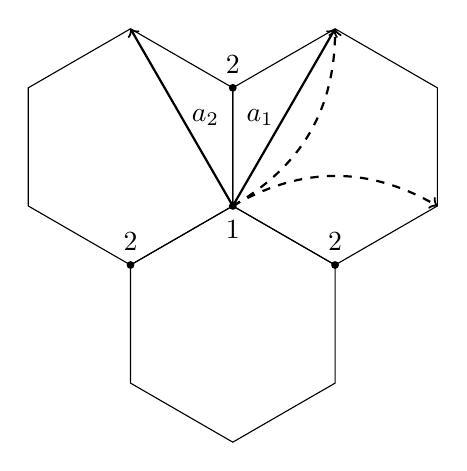
\begin{tikzpicture}
    \pgfmathsetmacro{\size}{1.5};
    \pgfmathsetmacro{\f}{sqrt(3)/2};
    \pgfmathsetmacro{\ss}{1/2};
    \draw (0,0) node[circle, inner sep=1pt, fill=black, label={below:$1$}]{};
    \draw (0,\size) node[circle, inner sep=1pt, fill=black, label={above:$2$}]{};
    \draw (\f*\size,-\ss*\size) node[circle, inner sep=1pt, fill=black, label={above:$2$}]{};
    \draw (-\f*\size,-\ss*\size) node[circle, inner sep=1pt, fill=black, label={above:$2$}]{};
    \draw (0,0) -- ++(\f*\size,-\ss*\size) -- ++(\f*\size,\ss*\size) -- ++(0, \size) -- ++(-\f*\size,\ss*\size) -- ++(-\f*\size,-\ss*\size) -- cycle;
    \draw (0,0) -- ++(0, \size) -- ++(-\f*\size,\ss*\size) -- ++(-\f*\size,-\ss*\size) --++(0, -\size) -- ++(\f*\size,-\ss*\size) -- ++(\f*\size,\ss*\size) -- cycle;
    \draw (0,0)  -- ++(-\f*\size,-\ss*\size) --++(0, -\size) -- ++(\f*\size,-\ss*\size) -- ++(\f*\size,\ss*\size) -- ++(0, \size) -- cycle;
    \draw[thick, ->] (0,0) -- node[left]{$\ve a_1$} ++(0+\f*\size, \size+\ss*\size);
    \draw[thick, ->] (0,0) -- node[right]{$\ve a_2$} ++(0-\f*\size, \size+\ss*\size);
    \path (0,0) edge[thick, draw, bend right, dashed, ->] ++(0+\f*\size, \size+\ss*\size);
    \path (0,0) edge[thick, draw, bend left, dashed, ->] ++(2*\f*\size, 0);
\end{tikzpicture}
\end{center}

The additional terms to \cref{eq:gp_graphene_H_nn} can be expressed as,
\[ H = \cdots -i t' \br{\ket{\ve R + \ve a_1 - \ve a_2, 1}\bra{\ve R, 1} - \ket{\ve R, 1} \bra{\ve R + \ve a_1 - \ve a_2, 1}} \cdots \]
Which has tunneling amplitude $i t'$. The intermediate negative sign is due to the tunneling amplitude being imaginary which switches signs under conjugation.\\


\subsubsection{Second Nearest-Neighbors}

\tikzstyle{atomoptions}=[draw, circle, inner sep=1pt, fill=#1]

\newcommand{\atomat}[2]{node[atomoptions={#1}] () at #2 {}}
\newcommand{\atom}[1]{\begin{tikzpicture}[baseline=-2pt]\draw\atomat{#1}{(0,0)};\end{tikzpicture}}
\newcommand{\hexgonat}[1]{
#1
-- ++(+\diagh,-\diagv)
-- ++(0, -\vert)
-- ++(-\diagh,-\diagv)
-- ++(-\diagh,+\diagv)
-- ++(0, +\vert)
-- ++(+\diagh,+\diagv)
}
\newcommand{\hexgonatatoms}[1]{
#1                  node[atomoptions={black}]{}
++(+\diagh,-\diagv) node[atomoptions={white}]{}
++(0, -\vert)       node[atomoptions={black}]{}
++(-\diagh,-\diagv) node[atomoptions={white}]{}
++(-\diagh,+\diagv) node[atomoptions={black}]{}
++(0, +\vert)       node[atomoptions={white}]{}
++(+\diagh,+\diagv) node[atomoptions={black}]{}
}
\newcommand{\atomm}{\atom{white}}
\newcommand{\atomp}{\atom{black}}

\begin{center}
\begin{tikzpicture}
    \pgfmathsetmacro{\edgelength}{1.5};
    \pgfmathsetmacro{\diagh}{sqrt(3)/2*\edgelength};
    \pgfmathsetmacro{\diagv}{1/2*\edgelength};
    \pgfmathsetmacro{\vert}{\edgelength};
    \pgfmathsetmacro{\feather}{0.2};
    \coordinate (a1) at (-\diagh, +\diagv+\vert);
    \coordinate (a2) at (+\diagh, +\diagv+\vert);
    \foreach \n/\m in {2/-1, -1/2, 2/0, 0/2, 0/-1,+1/-1,-1/0,0/0,+1/0,-1/+1,0/+1,+1/+1}{
        \draw[gray] \hexgonat{($\n*(a1) + \m*(a2)$)};
        \draw \hexgonatatoms{($\n*(a1) + \m*(a2)$)};
    }
    \foreach \n/\m in {2/-1, -1/2, 0/-1,+1/-1,-1/0,0/0,+1/0,-1/+1,0/+1, -1/-1, -2/+1, -2/+2, -2/0, +1/-2, +2/-2, 0/-2}{
        \draw[thick, red] plot [smooth cycle, tension=1, shift={($\n*(a1) + \m*(a2)$)}] coordinates {(-\feather,0) (+\feather,0) (+\feather,\vert) (-\feather,\vert)};
    }
    \draw[blue, fill=blue, fill opacity=0.05] \hexgonat{(0,+\vert)};
    \draw[<-] (+\diagh,0) to[in=0, out=0] (1,5) node[left]{Wigner-Seitz Unit Cell};
    \draw[thick, ->] (0,0) -- node[left ]{$\ve a_1$} ++(a1);
    \draw[thick, ->] (0,0) -- node[right]{$\ve a_2$} ++(a2);
    \draw[thick, dashed, green] (0, \vert) to[bend right] (-\diagh, -\diagv);
    \draw[thick, dashed, green] (0, \vert) to[bend right] (+\diagh, -\diagv);
    \draw[thick, dashed, green] (+\diagh, -\diagv) to[bend right] (0, \vert);
    \draw[thick, dashed, green] (+\diagh, -\diagv) to[bend left ] (-\diagh, -\diagv);
    \draw[thick, dashed, green] (-\diagh, -\diagv) to[bend right] (0, \vert);
    \draw[thick, dashed, green] (-\diagh, -\diagv) to[bend left ] (+\diagh, -\diagv);
    \draw[thick, dashed, green] (0,0) to[bend right] (a1);
    \draw[thick, dashed, green] (0,0) to[bend left ] (a2);
    \draw[thick, dashed, green] (0,0) to[bend left ] (a1);
    \draw[thick, dashed, green] (0,0) to[bend right] (a2);
    \draw[thick, dashed, green] (0,0) to[bend left ] ($-1*(a1) + 1*(a2)$);
    \draw[thick, dashed, green] (0,0) to[bend right] ($-1*(a1) + 1*(a2)$);
    \draw[thick, dashed, blue]  (0,0) to[bend left ] (0, \vert);
    \draw[thick, dashed, blue]  (0,0) to[bend left ] (+\diagh, -\diagv);
    \draw[thick, dashed, blue]  (0,0) to[bend left ] (-\diagh, -\diagv);
    \draw[thick, dashed, blue]  (0,0) to[bend right] (0, \vert);
    \draw[thick, dashed, blue]  (0,0) to[bend right] (+\diagh, -\diagv);
    \draw[thick, dashed, blue]  (0,0) to[bend right] (-\diagh, -\diagv);
\end{tikzpicture}
\end{center}
In the graphene lattice depicted above, each unit cell located at $\ve R = n_1 \ve a_1 + n_2 \ve a_2$ where $n_1, n_2 \in \Z$ has two atoms $\al \in \bc{\atomm, \atomp}$.
\[ \ve a_1 = \f{a}{2}\br{\hat x + \sqrt{3}\hat y} \qquad \ve a_2 = \f{a}{2}\br{-\hat x + \sqrt{3}\hat y} \]
An electron localized in the atom $\al \in \bc{\atomm, \atomp}$ at $\ve R$ is denoted as $\ket{\ve R, \al}$. \\

There are $6$ possible nearest-neighbor transitions illustrated in blue above. These transitions, with intensity $t_1$ can be written as the nearest-neighbor Hamiltonian $H_1$,
\[ H_1 = - t_1 \sum_{\ve R} \bc{\ket{\ve R, \atomm}\bra{\ve R, \atomp} + \ket{\ve R-\ve a_1, \atomm}\bra{\ve R, \atomp} + \ket{\ve R - \ve a_2, \atomm}\bra{\ve R, \atomp} + \text{h.c.}} \]
There are $12$ possible next-nearest-neighbor transitions illustrated in green above. These transitions, with intensity $t_2$ can be written as the nearest-neighbor Hamiltonian $H_2$ (note that these transitions were all defined in the same direction; this is important when we invoke $t_2 = i \ti t_2, \ti t_2 \in \R$ later),
\begin{align*}
H_{2, \atomm} &= - t_2 \sum_{\ve R} \bc{\ket{\ve R+\ve a_1, \atomm}\bra{\ve R, \atomm} + \ket{\ve R-\ve a_2, \atomm}\bra{\ve R, \atomm}+ \ket{\ve R-\ve a_1, \atomm}\bra{\ve R-\ve a_2, \atomm} + \text{h.c.}} \\
H_{2, \atomp} &= -t_2 \sum_{\ve R} \bc{\ket{\ve R+\ve a_1, \atomp}\bra{\ve R, \atomp} + \ket{\ve R, \atomp}\bra{\ve R+\ve a_2, \atomp}+ \ket{\ve R-\ve a_1, \atomp}\bra{\ve R-\ve a_2, \atomp} + \text{h.c.}}
\end{align*}
Altogether,
\[ H = H_1 + H_2 = H_1 + H_{2, \atomp} + H_{2, \atomm} \eq \label{eq:gp_hamiltonian_total}\]

In order to diagonalize \cref{eq:gp_hamiltonian_total} with respect to $\ve R$, we may switch to momentum space,
\[ \ket{\ve R, \al} =  \sum_{\ve R} \ket{\ve k, \al}\braket{\ve k, \al}{\ve R, \al} \qquad \forall \al \in \bc{\atomp, \atomm} \eq \label{eq:gp_basis_change}\]
Where $\braket{\ve k, \al}{\ve R, \al}$ is defined and normalized independent of $\al$. Motivated by free electrons, $\braket{k}{x} \propto e^{-ikx}$ we map $x$ to the position in the crystal:
\begin{align*}
    \eq \label{eq:gp_xk}
    \begin{split}
        x \mapsto n_1 \ve a_1 + n_2 \ve a_2 &= \ve R\\
        k \mapsto k_1 \f{\ve a_1}{a} + k_2 \f{\ve a_2}{a} &= \ve k
    \end{split}
\end{align*}
Therefore,
\[ \braket{\ve k, \al}{\ve R, \al} \propto e^{i\ve k \cdot \ve R} \eq \label{eq:gp_plane_wave}\]
The normalization factor comes from completeness,
\[ \sum_{\ve R} \abs{\braket{\ve k, \al}{\ve R, \al}}^2 = 1 \eq \label{eq:gp_normalization}\]
Heretofore, no restrictions have been made on the range of $\ve R$. Evidently, a real substance will possess finite, albeit many, unit cells. To emulate this feature, equip this model with periodic boundary conditions such that there are $N_i$ distinct unit cells in the $\ve a_i$ direction. Therefore for all $\al, \ve R$,
\[ \ket{\ve R, \al} = \ket{\ve R + N_1 \ve a_1, \al} = \ket{\ve R + N_2 \ve a_2, \al} \eq \label{eq:gp_periodic_boundary}\]
Letting $\ga \in \R$ be the normalization coefficient in \cref{eq:gp_plane_wave}, \cref{eq:gp_normalization} becomes,
\[ 1 = \sum_{\ve R} \abs{\braket{\ve k, \al}{\ve R, \al}}^2 = \sum_{n_1 = 1}^{N_1}\sum_{n_2 = 1}^{N_2} \abs{\ga e^{i\ve k \cdot \ve R}}^2 = N_1 N_2 \ga^2 \implies \ga = \f{1}{\sqrt{N_1 N_2}}\]
Consequently, \cref{eq:gp_basis_change} can be written as follows,
\[ \ket{\ve R, \al} = \f{1}{\sqrt{N_1N_2}} \sum_{\ve k} e^{i \ve k \cdot \ve R} \ket{\ve k, \al} \eq \label{eq:gp_basis_coeffs}  \]
Additionally, the periodic boundary condition of \cref{eq:gp_periodic_boundary} gives,
\[ \ket{\ve R, \al} = \ket{\ve R + N_i \ve a_i, \al} = \f{1}{\sqrt{N_1N_2}} \sum_{\ve k} e^{i \ve k \cdot \br{\ve R + N_i \ve a_i}} \ket{\ve k, \al} = \f{1}{\sqrt{N_1N_2}} \sum_{\ve k} e^{i \ve k \cdot \ve R} \ket{\ve k, \al}  \]
Therefore $e^{i N_i \ve k \cdot \ve a_i} = e^{i 2N_i k_i a} = 1$ which gives,
\[ 2N_i k_i a = 2 \pi m_i \qquad m_i \in \Z, \forall i \in \bc{1,2} \]
\[ k_i = \f{\pi m_i}{N_i a} \qquad m_i \in \Z, \forall i \in \bc{1,2} \eq \label{eq:gp_discrete_k} \]
Therefore each of the $k_i$'s are discrete. Summing \cref{eq:gp_hamiltonian_total} over the momentum space $\ve k, \ve k'$ and using the following identity,
\[ \f{1}{N_1 N_2} \sum_{\ve R} e^{-i\br{\ve k-\ve k'} \cdot \ve R} = \de_{\ve k, \ve k'} \]
Yields,
\begin{align*}
H_1 &= - t_1 \sum_{\ve k} \bc{\ket{\ve k, \atomm}\bra{\ve k, \atomp}\bc{1 + e^{-i \ve k \cdot \ve a_1} + e^{-i \ve k \cdot \ve a_2}} + \text{h.c.}} \\
H_{2, \atomm} &= - t_2 \sum_{\ve k} \bc{\ket{\ve k, \atomm}\bra{\ve k, \atomm}\bc{e^{i \ve k \cdot \ve a_1} + e^{-i \ve k \cdot \ve a_2} + e^{i \ve k \cdot \br{\ve a_2 - \ve a_1}}} + \text{h.c.}} \\
H_{2, \atomp} &= -t_2 \sum_{\ve k} \bc{\ket{\ve k, \atomp}\bra{\ve k, \atomp}\bc{e^{i \ve k \cdot \ve a_1} + e^{-i \ve k \cdot \ve a_2} + e^{i \ve k \cdot \br{\ve a_2 - \ve a_1}}} + \text{h.c.}}
\end{align*}
Therefore $H = \sum_{\ve k}H\br{\ve k}$ gives,
\[ H\br{\ve k} = \sum_{\ve k} \br{-t_1  \bs{\ket{\atomm}\bra{\atomp}\bc{1 + e^{-i \ve k \cdot \ve a_1} + e^{-i \ve k \cdot \ve a_2}}} - t_2\bs{\br{\ket{\atomp}\bra{\atomp} + \ket{\atomm}\bra{\atomm}}\bc{e^{i \ve k \cdot \ve a_1} + e^{-i \ve k \cdot \ve a_2} + e^{i \ve k \cdot \br{\ve a_2 - \ve a_1}}}}} + \text{h.c.}    \]

Since $H\br{\ve k}$ is a two-level system $\bc{\ket{\atomp, \atomm}}$ we invoke a pseudo-spin denoted by the Pauli matrices $\ve \si$.

\begin{align*}
    \ve \si &= \br{\si^{x}, \si^{y}, \si^{z}} \\
    \si^{z} &= \ket{\atomp} \bra{\atomp} - \ket{\atomm}\bra{\atomm} \\
    \si^{y} &= -i\br{\ket{\atomp} \bra{\atomm} - \ket{\atomm}\bra{\atomp}} \\
    \si^{x} &= \ket{\atomp} \bra{\atomm} + \ket{\atomm}\bra{\atomp}
\end{align*}
Therefore $\ket{\atomp} \bra{\atomm}$ can be written as follows,
\[ \ket{\atomp} \bra{\atomm} = \f{1}{2}\bc{\si^{x} + i \si^{y}} \qquad \ket{\atomm} \bra{\atomp} = \f{1}{2}\bc{\si^{x} - i \si^{y}} \]
Since $t_1 \in \R$, this implies,
\begin{align*}
    \ket{\atomm}\bra{\atomp}\bc{1 + e^{-i \ve k \cdot \ve a_1} + e^{-i \ve k \cdot \ve a_2}} + \text{h.c.}
    &= \ket{\atomm}\bra{\atomp}\bc{1 + e^{-i \ve k \cdot \ve a_1} + e^{-i \ve k \cdot \ve a_2}} + \ket{\atomp}\bra{\atomm}\bc{1 + e^{i \ve k \cdot \ve a_1} + e^{i \ve k \cdot \ve a_2}}\\
    &= \f12\br{\si^{x} - i \si^{y}}\bc{1 + e^{-i \ve k \cdot \ve a_1} + e^{-i \ve k \cdot \ve a_2}} + \f12\br{\si^{x} + i \si^{y}}\bc{1 + e^{i \ve k \cdot \ve a_1} + e^{i \ve k \cdot \ve a_2}}\\
    &= \si^{x}\br{1 + \cos \br{\ve k \cdot \ve a_1} + \cos \br{\ve k \cdot \ve a_2}} + \si^{y}\br{\sin \br{\ve k \cdot \ve a_1} + \sin \br{\ve k \cdot \ve a_2}}
\end{align*}
In contrast, if $t_2$ is imaginary $t_2^{*} = - t_2$ which means $t_2 = i \ti t_2$,
\begin{align*}
    &t_2\underbrace{\br{\ket{\atomp}\bra{\atomp} + \ket{\atomm}\bra{\atomm}}}_{\ident}\bc{e^{i \ve k \cdot \ve a_1} + e^{-i \ve k \cdot \ve a_2} + e^{i \ve k \cdot \br{\ve a_2 - \ve a_1}}} +\text{h.c.} \\
    &\qquad= i\ti t_2\bc{e^{i \ve k \cdot \ve a_1} + e^{-i \ve k \cdot \ve a_2} + e^{i \ve k \cdot \br{\ve a_2 - \ve a_1}}} +\text{h.c.} \\
    &\qquad= i\ti t_2\bc{e^{i \ve k \cdot \ve a_1} + e^{-i \ve k \cdot \ve a_2} + e^{i \ve k \cdot \br{\ve a_2 - \ve a_1}} - e^{-i \ve k \cdot \ve a_1} - e^{i \ve k \cdot \ve a_2} - e^{-i \ve k \cdot \br{\ve a_2 - \ve a_1}}} \\
    &\qquad= 2\ti t_2\bc{\sin\br{-\ve k \cdot \ve a_1} + \sin\br{\ve k \cdot \ve a_2} + \sin\br{\ve k \cdot \br{\ve a_1 - \ve a_2}}}
\end{align*}

In order to write $H_{2, \atomp}$ in terms of $\ve d\br{\ve k} \cdot \ve \si$, recognize that if the electrons have spin,
\begin{align*}
    \ve s &= \br{s^{x}, s^{y}, s^{z}} \\
    s^{z} &= \ket{\uparrow} \bra{\uparrow} - \ket{\downarrow}\bra{\downarrow} \\
    s^{y} &= -i\br{\ket{\uparrow} \bra{\downarrow} - \ket{\downarrow}\bra{\uparrow}} \\
    s^{x} &= \ket{\uparrow} \bra{\downarrow} + \ket{\downarrow}\bra{\uparrow}
\end{align*}
Then the eigenstates can become the following,
\[ \ket{\ve R, \al} \mapsto \ket{\ve R, \al_{\si}, \al_{s}} \qquad \al_{\si} \in \bc{\atomm, \atomp} , \al_{s} \in \bc{\uparrow, \downarrow} \]
Then is is possible to write the following,
\[ \ident = s^{z} \si^{z} \]
Therefore,
\begin{align*}
    d^{x}\br{\ve k} &= -t_1\bc{1 + \cos \br{\ve k \cdot \ve a_1} + \cos \br{\ve k \cdot \ve a_2}} \\
    d^{y}\br{\ve k} &= -t_1\bc{\sin \br{\ve k \cdot \ve a_1} + \sin \br{\ve k \cdot \ve a_2}}\\
    d^{z}\br{\ve k} &= 2\ti t_2s^{z}\bc{\sin\br{-\ve k \cdot \ve a_1} + \sin\br{\ve k \cdot \ve a_2} + \sin\br{\ve k \cdot \br{\ve a_1 - \ve a_2}}}
\end{align*}
In terms of the $x,y$ components of $\ve k$,
\[ \ve k = k_x \hat x + k_y \hat y  \]
\[ \ve a_1 = \f{a}{2}\br{\hat x + \sqrt{3}\hat y} \qquad \ve a_2 = \f{a}{2}\br{-\hat x + \sqrt{3}\hat y} \eq \label{eq:gp_graphene_a}\]
\begin{align*}
\eq \label{eq:gp_kxky}
\begin{split}
\ve k \cdot \ve a_1 &= \br{k_x \hat x + k_y \hat y}\br{\f{a}{2}\br{\hat x + \sqrt{3}\hat y}} = \f{a}{2}\br{k_x + \sqrt{3}k_y} \\
\ve k \cdot \ve a_2 &= \br{k_x \hat x + k_y \hat y}\br{\f{a}{2}\br{-\hat x + \sqrt{3}\hat y}} = \f{a}{2}\br{-k_x + \sqrt{3}k_y}
\end{split}
\end{align*}
Trig identities give,
\begin{align*}
    d^{x}\br{\ve k} &= -t_1\bc{1 + 2 \cos \br{\f{ak_x}{2}}\cos \br{\f{\sqrt{3}ak_y}{2}}} \\
    d^{y}\br{\ve k} &= -2t_1\bc{\cos \br{\f{ak_x}{2}}\sin \br{\f{\sqrt{3}ak_y}{2}}}\\
    d^{z}\br{\ve k} &= -2\ti t_2s^{z}\bc{-2 \sin \br{\f{ak_x}{2}}\cos \br{\f{\sqrt{3}ak_y}{2}} + \sin\br{k_x a}}\\
\end{align*}
The energy dispersion relations are,
\[ \vep\br{\ve k} = \pm\abs{\ve d\br{\ve k}} \]
\begin{align*}
\eq \label{eq:gp_dispersion}
\vep_{\pm}\br{\ve k}
&= \pm \bigg(t_1^2\bc{1 + 2 \cos \br{\f{ak_x}{2}}\cos \br{\f{\sqrt{3}ak_y}{2}}}^2 + \cdots \\
&\cdots + 4t_1^2\bc{\cos \br{\f{ak_x}{2}}\sin \br{\f{\sqrt{3}ak_y}{2}}}^2 + \cdots \\
&\cdots + 4\ti t_2^2{s^{z}}^2\bc{-2 \sin \br{\f{ak_x}{2}}\cos \br{\f{\sqrt{3}ak_y}{2}} + \sin\br{k_x a}}^2\bigg)^{1/2}
\end{align*}

By examining these equations it can be seen that there are two points (and only two points) in the first Brillouin zone where both $d^{x}$ and $d^y$ vanish simultaneously (at least in the case where $\ti t_2 = 0$). We label these points as $\ve k_{\pm}$,
\[ \ve k_+ = \br{k_{+, x}, k_{+, y}} = \br{\f{4 \pi }{3a}, 0} \]
\[ \ve k_- = \br{k_{-, x}, k_{-, y}} = \br{-\f{4 \pi }{3a}, 0} \]
Therefore, in the limit where $\ve k \simeq \ve k_{\pm}$,
\[ \ve k = \ve k_{\pm} + \de \ve k_{\pm} \]
Therefore in the limit that $\de \ve k_{\pm} \simeq \ve 0$,
\begin{align*}
    \cos \br{ak_x} &= \cos \br{ak_{\pm,x} + a\de k_{\pm,x}} \\
    &= \cos \br{ak_{\pm,x}}\cos \br{a\de k_{\pm,x}} - \sin \br{ak_{\pm,x}}\sin \br{a\de k_{\pm,x}} \\
    &= \cos \br{\f{4\pi}{3}}\cos \br{a\de k_{\pm,x}} - \sin \br{\pm\f{4\pi}{3}}\sin \br{a\de k_{\pm,x}} \\
    &= -\f12\cos \br{a\de k_{\pm,x}} \pm \f{\sqrt{3}}{2}\sin \br{a\de k_{\pm,x}} \\
    &\simeq -\f{1}{2} \pm \f{\sqrt{3}}{2}a\de k_{\pm,x} \\
    \sin \br{ak_x} &= \sin \br{ak_{\pm,x} + a\de k_{\pm,x}} \\
    &= \cos \br{ak_{\pm,x}}\sin \br{a\de k_{\pm,x}} + \sin \br{ak_{\pm,x}}\cos \br{a\de k_{\pm,x}}\\
    &= \cos \br{\f{4\pi}{3}}\sin \br{a\de k_{\pm,x}} + \sin \br{\pm\f{4\pi}{3}}\cos \br{a\de k_{\pm,x}} \\
    &= -\f12\sin \br{a\de k_{\pm,x}} \mp \f{\sqrt{3}}{2}\cos \br{a\de k_{\pm,x}} \\
    &\simeq -\f{1}{2}a\de k_{\pm,x} \mp \f{\sqrt{3}}{2} \\
    \cos \br{\f{ak_x}{2}} &= \cos \br{\f{ak_{\pm,x}}{2} + \f{a\de k_{\pm,x}}{2}} \\
    &= \cos \br{\f{ak_{\pm,x}}{2}}\cos \br{\f{a\de k_{\pm,x}}{2}} - \sin \br{\f{ak_{\pm,x}}{2}}\sin \br{\f{a\de k_{\pm,x}}{2}} \\
    &= \cos \br{\f{2 \pi}{3}}\cos \br{\f{a\de k_{\pm,x}}{2}} - \sin \br{\pm\f{2 \pi}{3}}\sin \br{\f{a\de k_{\pm,x}}{2}} \\
    &= -\f{1}{2}\cos \br{\f{a\de k_{\pm,x}}{2}} \mp \f{\sqrt{3}}{2}\sin \br{\f{a\de k_{\pm,x}}{2}} \\
    &\simeq -\f{1}{2} \mp \f{\sqrt{3}}{2}\f{a\de k_{\pm,x}}{2} \\
    \sin \br{\f{ak_x}{2}} &= \sin \br{\f{ak_{\pm,x}}{2} + \f{a\de k_{\pm,x}}{2}} \\
    &= \cos \br{\f{ak_{\pm,x}}{2}}\sin \br{\f{a\de k_{\pm,x}}{2}} + \sin \br{\f{ak_{\pm,x}}{2}}\cos \br{\f{a\de k_{\pm,x}}{2}} \\
    &= \cos \br{\f{2 \pi}{3}}\sin \br{\f{a\de k_{\pm,x}}{2}} + \sin \br{\pm \f{2 \pi}{3}}\cos \br{\f{a\de k_{\pm,x}}{2}} \\
    &= -\f{1}{2}\sin \br{\f{a\de k_{\pm,x}}{2}} \pm \f{\sqrt{3}}{2}\cos \br{\f{a\de k_{\pm,x}}{2}} \\
    &\simeq -\f{1}{2}\f{a\de k_{\pm,x}}{2} \pm \f{\sqrt{3}}{2} \\
    \cos \br{\f{\sqrt{3}ak_y}{2}}
    &= \cos \br{\f{\sqrt{3}a\de k_{\pm,y}}{2}} \\
    &\simeq 1
\end{align*}
Therefore to first order,
\begin{align*}
    d_{\pm}^{x}\br{\ve k} &\simeq -t_1\bc{1 + 2\br{-\f{1}{2} \mp \f{\sqrt{3}}{2}\f{a\de k_{\pm,x}}{2}}} \\
    d_{\pm}^{y}\br{\ve k} &\simeq -2t_1\bc{\br{-\f{1}{2} \mp \f{\sqrt{3}}{2}\f{a\de k_{\pm,x}}{2}}\f{\sqrt{3}a\de k_{\pm, y}}{2}}\\\
    d_{\pm}^{z}\br{\ve k} &\simeq 2\ti t_2s^{z}\bc{-2 \br{-\f{1}{2}\f{a\de k_{\pm,x}}{2} \mp \f{\sqrt{3}}{2}} + \br{-\f{1}{2}a\de k_{\pm,x} \pm \f{\sqrt{3}}{2}}}
\end{align*}
Simplifying
\begin{align*}
    d_{\pm}^{x}\br{\ve k} &\simeq \pm \f{at_1 \sqrt{3}\de k_{\pm,x}}{2} \\
    d_{\pm}^{y}\br{\ve k} &\simeq \f{at_1 \sqrt{3}\de k_{\pm,y}}{2}\\
    d_{\pm}^{z}\br{\ve k} &\simeq \pm 3\sqrt{3}t_2s^{z}
\end{align*}

This new degree of freedom, namely whether or not the electron is near $\ve k_{+}$ or $\ve k_{-}$ can be expressed as another pseudo-spin $\tau$,
\begin{align*}
    \ve \tau &= \br{\tau^{x}, \tau^{y}, \tau^{z}} \\
    \tau^{z} &= \ket{+} \bra{+} - \ket{-}\bra{-} \\
    \tau^{y} &= -i\br{\ket{+} \bra{-} - \ket{-}\bra{+}} \\
    \tau^{x} &= \ket{+} \bra{-} + \ket{-}\bra{+}
\end{align*}
Moreover a unique constant emerges as the Fermi velocity $v\tsb{F}$,
\[ \hbar v\tsb{F} = \f{at_1 \sqrt{3}}{2}\]
Thus $H\br{\ve k}$ becomes,
\begin{align*}
H\br{\ve k}
&= \si^{x}d^{x}\br{\ve k} + \si^{y}d^{y}\br{\ve k} + \si^{z}d^{z}\br{\ve k} \\
&= \hbar v\tsb{F}\br{\tau^{z}\si^{x}\de k_{x} + \si^{y} \de k_{y}} + 3\sqrt{3} \ti t_2 \si^{z} \tau^{z} s^{z}
\end{align*}
Finally, suppress the notation `$\de$' and define the spin orbital coupling $\De\tsb{SO}$.
\[ \De\tsb{SO} = 3 \sqrt{3} \ti t_2 \]
Therefore near $\ve k \simeq \ve k_{\pm}$,
\[ H\br{\ve k} = \hbar v\tsb{F}\br{\tau^{z}\si^{x}k_{x} + \si^{y} k_{y}} + \De\tsb{SO} \si^{z} \tau^{z} s^{z} \]
This Hamiltonian has the desired invariant spin terms $\si^{z} \tau^{z} s^{z}$ and should have been expected due to symmetry due to symmetries.

\subsubsection{Spin-Orbit Interactions Analyzed}

In order to study the effect $\De\tsb{SO}$ in \cref{eq:gp_kane_mele}, we will include a massive term $m \si^{z}$ and study the following,
\[ H\br{\ve k} =\hbar v\tsb{F} \br{k_x \tau^{z} \si^x + k_y \si^{y}} + \De\tsb{SO} \tau^{z} \si^{z} S^{z} + m \si^{z}\]
Specifically for our analysis, we will look at the affect on $S^{z} = 1$ spin up ($\uparrow$) spins. The associated Hamiltonian for $S^{z} = 1$ has two bands $\tau^{z} = \pm 1$,
\[ \bc{H\br{\ve k}}_{\tau^{z} = +1} \defined H_{+}\br{\ve k} =\hbar v\tsb{F} \br{k_x \si^x + k_y \si^{y}} + \br{m + \De\tsb{SO}} \si^{z}\]
\[ \bc{H\br{\ve k}}_{\tau^{z} = -1} \defined H_{+}\br{\ve k} =\hbar v\tsb{F} \br{-k_x \si^x + k_y \si^{y}} + \br{m - \De\tsb{SO}} \si^{z}\]
Therefore the dispersion relations are distinct for each value of $\tau^{z}$,
\begin{align*}
    \bc{\vep\br{\ve k}}_{\tau^{z} = +1}\defined \vep_{+}\br{\ve k} &= \pm\sqrt{\hbar^2 v\tsb{F}^2 \br{k_x^2 + k_y^2} + \br{m + \De\tsb{SO}}^2} \\
    \bc{\vep\br{\ve k}}_{\tau^{z} = -1}\defined \vep_{-}\br{\ve k} &= \pm\sqrt{\hbar^2 v\tsb{F}^2 \br{k_x^2 + k_y^2} + \br{m - \De\tsb{SO}}^2} \eq \label{eq:gp_SOminus}
\end{align*}
In the very large $m$ limit $m \gg \De\tsb{SO}$, the energy cost $(+m)$ for electrons being localized at sites of type $1$ is much higher than the energy cost $(-m)$ associated with sites of type $2$. Therefore all of the electrons will localize to sites of type $2$. Therefore in this case, the electrons can not propagate between sites because the atoms of type $1$ are in the way. We refer to these as \term{non-topological insulators} or sometimes \textit{atomic} insulators. \\

In contrast to this, in the region where $m \approx \De\tsb{SO}$ we have interesting behaviors for \cref{eq:gp_SOminus}. Since the band gap associated with the contribution from $\vep_{-}\br{\ve k}$ is $2 \abs{m - \De\tsb{SO}}$, the band gap closes when $m$ transitions between $m > \De\tsb{SO}$ and $m < \De\tsb{SO}$.
\begin{itemize}
    \item $m > \De\tsb{SO}$: Trivial insulator
    \item $m = \De\tsb{SO}$: Transition point/semimetal
    \item $m < \De\tsb{SO}$: Topological insulator
\end{itemize}
We have already seen this behavior for graphene in which $m=0$ defined a semimetal, and $m>0$ defined a topological insulator form of graphene. Recall the Hamiltonian of graphene had the following form,
\[ H\br{\ve k} = \ve d \br{\ve k} \cdot \ve \si \]
The unit vector of $\ve d$ is,
\[ \hat d \br{\ve k} = \f{\ve d \br{\ve k}}{\abs{\ve d \br{\ve k}}} \]
Which can be thought of as a map from the first Brillouin zone ($\ve k$) to the surface of a unit sphere $\hat d$. Interpreting the mappings in the way always one to understand the topological differences between ordinary and topological insulators. \\

Near the band touching points $\ve k_{\pm}$ we have,
\[ \hat d\br{\ve k_{+}} = \f{\br{\hbar v\tsb{F} k_x,\hbar v\tsb{F} k_y, m+\De\tsb{SO}}}{\sqrt{\hbar^2 v\tsb{F}^2 \br{\ve k_x^2 + \ve k_y^2 } + \br{m + \De\tsb{SO}}^2}} \]
\[ \hat d\br{\ve k_{-}} = \f{\br{-\hbar v\tsb{F} k_x,\hbar v\tsb{F} k_y, m-\De\tsb{SO}}}{\sqrt{\hbar^2 v\tsb{F}^2 \br{\ve k_x^2 + \ve k_y^2 } + \br{m + \De\tsb{SO}}^2}} \]
Clearly for the case of $m > \De\tsb{SO}$,
\[ \ve d\br{\ve k_{-}} \cdot \hat z = m - \De\tsb{SO} > 0 \]
Therefore $d^z\br{\ve k_{-}}$ is always positive. This is also true for $d\br{\ve k}$. Therefore $\ve d\br{\ve k}$ only covers the \textit{upper} hemisphere of the unit sphere as $\ve k$ covers the whole Brillouin zone.\\

In difference to this is the case for $m < \De\tsb{SO}$. $d^{z}\br{\ve k_{-}}$ is always negative which means that $\hat d\br{\ve k}$ is able to cover the entire sphere.\\

Given this observation, we can define the following \term{topological invariant} that characterizes the difference between topological insulators and ordinary insulators. This quantity is the integer $n \in \bc{0,1}$ defined as,
\[ n = \f{1}{4\pi} \int_{\text{BZ}} \dif^2 k \hat d\cdot \br{\di_{k_x} \hat d \times \di_{k_y} \hat d} = \begin{cases}
    1 & \text{Topological Insulators} \\
    0 & \text{Normal Insulators} \\
\end{cases} \]
Where $\int_{\text{BZ}}$ refers to an integration over the entire Brillouin zone (BZ). \\


\subsubsection{Topological/Non-topological Interfaces}

Topological insulators behave exactly like insulators except that electrons near the band touching points have the potential to transition to the upper band and permit conduction. In order to study this in detail, it s sufficient to consider the Hamiltonian component associated with the topological terms,
\[ H_{-}\br{\ve k} = \hbar v\tsb{F}\br{- k_x \si^{x} +k_y \si^{y}} + \br{m - \De\tsb{SO}} \si^{z} \]
Where the coefficient in front of $\si^{z}$ differs in sign depending on whether or not the insulator is topological or not. Let us assume that we have a material that transitions from a topological insulator to an ordinary insulator by letting $m\br{x}$ denote the coefficient in front of $\si^{z}$ as it varies along the $x$-direction.
\[ m\br{x} = m - \De\tsb{SO}\]
Since $k_x$ no-longer corresponds to plane wave solutions to the Schrodinger equation, we replace $k_x$ with its representation in position space,
\[ k_x \mapsto - i\pder{}{x} \]
And solve $H\br{k_y}$,
\[ H\br{k_y} = i \hbar v\tsb{F} \pder{}{x} \si^{x} + \hbar v\tsb{F} k_y \si^{y} + m\br{x} \si^{z} \]
As a preliminary exercise, we can solve the Schrodinger equation for the case of $k_y = 0$.
\[ H\br{0} = i \hbar v\tsb{F} \pder{}{x} \si^{x} + m\br{x} \si^{z} \eq \label{eq:gp_kyzero} \]
For the zero energy eigenstate we require $H\psi = 0$. This suggests the following ansatz solution (for some unspecified $\ket{z}$),
\[ \psi\br{x} = e^{f\br{x}} \si^{x} \ket{z} \eq \label{eq:gp_ansatzxx}\]
Substituting \cref{eq:gp_ansatzxx} into \cref{eq:gp_kyzero} and making use of the fact that $\si^{z} \si^{x} = i\si^{y}$,
\[ \br{i \hbar v\tsb{F} \der{f}{x} + i m\br{x} \si^{y}} e^{f\br{x}} \ket{z} = 0 \]
Therefore,
\[ \br{\der{f}{x} + \f{m\br{x}}{\hbar v\tsb{F}} \si^{y}} \ket{z} = 0 \]
If we choose $\ket{z}$ such that $\si^{y}\ket{z} = \ket{z}$.
\[ \der{f}{x} = - \f{m\br{x}}{\hbar v\tsb{F}} \implies f\br{x} = - \f{1}{\hbar v\tsb{F}} \int_{0}^{x} \dif x' m\br{x'} \]
Therefore,
\[ \psi\br{x} = e^{- \f{1}{\hbar v\tsb{F}} \int_{0}^{x} \dif x' m\br{x'}} \si^{x} \ket{z} \]
What is $\si^{x} \ket{z}$?
\[ \si^{y}\si^{x} \ket{z} = -\si^{x}\si^{y} \ket{z} = - \si^{x}\ket{z} \]
Therefore $\si^{x}\ket{z}$ is an eigenstate of $\si^{y}$ with eigenvalue $-1$. Therefore,
\[ \psi\br{x} = e^{- \f{1}{\hbar v\tsb{F}} \int_{0}^{x} \dif x' m\br{x'}}\ket{\si^{y} = -1} \eq \label{eq:jackiv_relli}\]
This is the zero-energy eigenstate of the Hamiltonian localized at $x = 0$ for the special case of $k_y = 0$.
The eigenstate of \cref{eq:jackiv_relli} is know in high energy physics as the Jackiv-Relli solution.
If we consider cases where $k_y \neq 0$ we have,
\[ H\br{k_y} \psi\br{x} = \hbar v\tsb{F} k_y \si^{y} \psi\br{x} = - \hbar v\tsb{F} k_y \psi\br{x} \]
Which means $\psi\br{x}$ is an eigenstate of $H\br{k_y}$ with energy $- \hbar v\tsb{F} k_y$. The dispersion relation is,
\[ \vep\br{k_y} = - \hbar v\tsb{F} k_y \eq \label{eq:chrial_dispersion}\]
\begin{center}
\begin{tikzpicture}
    \pgfmathsetmacro{\axissize}{3};
    \draw[->] (-\axissize,0) -- (+\axissize,0) node[right]{$k_y$};
    \draw[->] (0, -\axissize) -- (0,+\axissize) node[above]{$\vep$};
    \draw[blue, thick] (-1, 3) -- (+1, -3);
    \draw[<-] (-0.5, 1.5) to[out=20, in=200] (2, 2) node[right]{slope $\hbar v\tsb{F}$};
\end{tikzpicture}
\end{center}
We refer to this type of dispersion as \term{chiral dispersion}. To understand why we refer to this as chiral dispersion, recall some properties of relativistic quantum mechanics. The velocity of free electrons is,
\[ \vep\br{\ve k} = \f{\hbar^2 k^2}{2 m} \eq \label{eq:free_electron_velocity}\]
This can be derived using classical intuition,
\[ \ve v = \f{\ve p}{m} = \f{\hbar \ve k}{m} \eq \label{eq:general_velocity}\]
Of course, \cref{eq:free_electron_velocity} and \cref{eq:general_velocity} only hold for free electrons. More generally, we can define the \term{group velocity},
\[ \ve v = \f{1}{\hbar} \vdel_{\ve k} \vep\br{\ve k} \eq \label{eq:group_velocity}\]
For \cref{eq:chrial_dispersion} we have,
\[ \ve v = - v\tsb{F} \hat y \]
Which means that all the electrons move in one direction. This is in contrast with an ordinary conductor where electrons have the ability to propagate in point directions subject to an external potential.

\subsubsection{Quantum Spin Hall Effect}

Using alternating external potentials $V_y$ we can construct and consider a 2D metal where the electrons move in alternating directions.
\begin{center}
    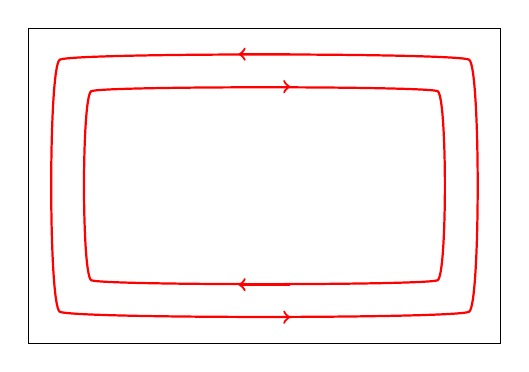
\begin{tikzpicture}
        \pgfmathsetmacro{\hL}{3};
        \pgfmathsetmacro{\vL}{2};
        \pgfmathsetmacro{\s}{0.4};
        \pgfmathsetmacro{\ss}{0.33};
        \draw (- \hL, - \vL) -- (- \hL, + \vL);
        \draw (- \hL, + \vL) -- (+ \hL, + \vL);
        \draw (+ \hL, + \vL) -- (+ \hL, - \vL);
        \draw (+ \hL, - \vL) -- (- \hL, - \vL);
        \draw [thick, red] plot [smooth cycle, tension=0.1] coordinates {(- \hL + 1*\s, - \vL+ 1*\s) (- \hL+ 1*\s, + \vL- 1*\s) (+ \hL- 1*\s, + \vL- 1*\s) (+ \hL- 1*\s, - \vL+ 1*\s)};
        \draw [thick, red, ->] (+1*\ss, + \vL - 1*\ss) -- (-1*\ss, + \vL - 1*\ss);
        \draw [thick, red, ->] (-1*\ss, - \vL + 1*\ss) -- (+1*\ss, - \vL + 1*\ss);
        \draw [thick, red] plot [smooth cycle, tension=0.1] coordinates {(- \hL + 2*\s, - \vL+ 2*\s) (- \hL+ 2*\s, + \vL- 2*\s) (+ \hL- 2*\s, + \vL- 2*\s) (+ \hL- 2*\s, - \vL+ 2*\s)};
        \draw [thick, red, ->] (-1*\ss, + \vL - 2.25*\ss) -- (+1*\ss, + \vL - 2.25*\ss);
        \draw [thick, red, ->] (+1*\ss, - \vL + 2.25*\ss) -- (-1*\ss, - \vL + 2.25*\ss);
    \end{tikzpicture}
\end{center}
This metal produces the \term{quantum spin hall effect}. We can define the current density $\ve j$,
\[ \ve j = - e n \ve v \]
Where $n$ is the density of the electrons which can be written as a integral over momentum space.
Doing so gives the current where the electrons move to the right as,
\[ I_R = - e \int v\tsb{F} n\tsb{F}\br{\vep_k} \f{\dif k_x}{2 \pi} \]
Where $k = 2\pi n / L$ and $2\pi / L$ is the volume in momentum space corresponding to a single quantum state.
\[ \f{1}{L} \f{\dif k_x}{\f{2 \pi }{L}} = \f{\dif k_x}{2 \pi} \]
If we convert this integral from an integral over momentum space to and integral over energies,
\[ \vep = \hbar v\tsb{F} k_x \implies \dif k_x = \f{\dif \vep}{\hbar v\tsb{F}} \]
Therefore the current is,
\[ I_{R} = - e v\tsb{F}  \f{1}{2\pi \hbar v\tsb{F}} \int_{-\inf}^{\vep_{FR}} \dif \vep = - \f{e}{h} \int_{-\inf}^{\vep_{FR}} \dif \vep \]
Where $\vep_{FR}$ is the Fermi energy for the right-traveling electrons.
The current for the electrons traveling to the left is opposite in sign,
\[ I_L = \f{e}{h} \int_{-\inf}^{\vep_{FL}} \dif \vep \]
Therefore the net current is,
\[ I = I_{R} + I_{L} = - \f{e}{h} \int_{\vep_{FL}}^{\vep_{FR}} \dif \vep = - \f{e}{h} \br{\vep_{FR} - \vep_{FL}} = - \f{e^2}{h} V_{y} \]
The conductivity is,
\[ \f{I}{V_{y}} = - \f{e^2}{h} \]
The interesting feature of this conductivity is that is only depends on the fundamental constants $e, h$. As it turns out, measurements of this conductivity represent our most precise measurements of $e$ and $h$. An excellent external resource is a book by R.B. Laughlin called \textit{Different Universe}. An important thing to remember that this analysis only applies for a particular spin value. In this case we analyzed spin up states $S^{z} = +1$. In general we have,
\[ \si_{xy}^{\uparrow} = -\f{e^2}{h} \qquad \si_{xy}^{\downarrow} = +\f{e^2}{h} \]
Which means that we can construct a \term{spin current},
\[ \si_{xy}^{S} =\f{1}{2} \br{\si_{xy}^{\uparrow} - \si_{xy}^{\downarrow}} = - \f{e^2}{h} \]
Effectively, if we have an equal number of electrons moving to the right and the left but each direction is biased to a particular spin, we can have a buildup of spin up electrons on the right and spin down electrons on the left. This is the analogue of \textit{spin voltage}. \\

\subsection{Bravais Lattices in 3D}

There are a number of typical Bravais lattices in three dimensions. The simplest one is the simple cubic.
\begin{enumerate}
    \item \term{Simple Cubic}:
    \begin{center}
        \begin{tikzpicture}
        \pgfmathsetmacro{\axissize}{1};
        \pgfmathsetmacro{\shiftx}{-4};
        \pgfmathsetmacro{\shifty}{0};
        \pgfmathsetmacro{\shiftz}{0};
        \draw[->] (\shiftx,\shifty, \shiftz) -- (\shiftx+\axissize,\shifty, \shiftz) node[right]{$y$};
        \draw[->] (\shiftx,\shifty, \shiftz) -- (\shiftx,\shifty+\axissize, \shiftz) node[above]{$z$};
        \draw[->] (\shiftx,\shifty, \shiftz) -- (\shiftx,\shifty, \shiftz+\axissize) node[below left]{$x$};
        \foreach \uda in {-1,+1}
        \foreach \udb in {-1,+1}
        \draw[gray, dashed]
        (-1,+\uda,+\udb) -- (+1,+\uda,+\udb)
        (+\uda,-1,+\udb) -- (+\uda,+1,+\udb)
        (+\uda,+\udb,-1) -- (+\uda,+\udb,+1)
        ;
        \foreach \x in {-1,+1}
        \foreach \y in {-1,+1}
        \foreach \z in {-1,+1}
        \draw[] (\x,\y,\z) node[fill=black, circle, inner sep=1pt]{};
        \draw[->] (-1,-1,-1) -- (+1,-1,-1) node[right]{$\ve a_2$};
        \draw[->] (-1,-1,-1) -- (-1,+1,-1) node[above]{$\ve a_3$};
        \draw[->] (-1,-1,-1) -- (-1,-1,+1) node[below left]{$\ve a_1$};
        \end{tikzpicture}
    \end{center}
    \[ \ve a_1 = a \hat x \quad \ve a_2 = a \hat y \quad \ve a_3 = a \hat z \]
    \item \term{Body-centered Cubic (bcc)}:
    \begin{center}
        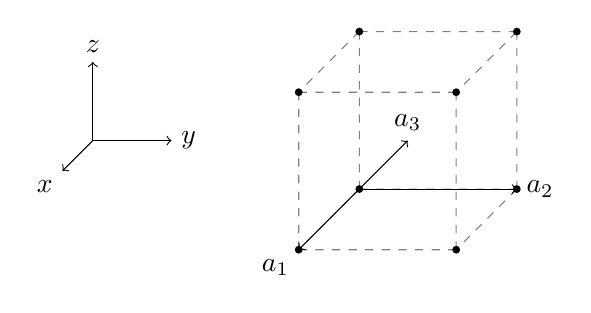
\begin{tikzpicture}
        \pgfmathsetmacro{\axissize}{1};
        \pgfmathsetmacro{\shiftx}{-4};
        \pgfmathsetmacro{\shifty}{0};
        \pgfmathsetmacro{\shiftz}{0};
        \draw[->] (\shiftx,\shifty, \shiftz) -- (\shiftx+\axissize,\shifty, \shiftz) node[right]{$y$};
        \draw[->] (\shiftx,\shifty, \shiftz) -- (\shiftx,\shifty+\axissize, \shiftz) node[above]{$z$};
        \draw[->] (\shiftx,\shifty, \shiftz) -- (\shiftx,\shifty, \shiftz+\axissize) node[below left]{$x$};
        \foreach \uda in {-1,+1}
        \foreach \udb in {-1,+1}
        \draw[gray, dashed]
        (-1,+\uda,+\udb) -- (+1,+\uda,+\udb)
        (+\uda,-1,+\udb) -- (+\uda,+1,+\udb)
        (+\uda,+\udb,-1) -- (+\uda,+\udb,+1)
        ;
        \foreach \x in {-1,+1}
        \foreach \y in {-1,+1}
        \foreach \z in {-1,+1}
        \draw[] (\x,\y,\z) node[fill=black, circle, inner sep=1pt]{};
        \draw[->] (-1,-1,-1) -- (+1,-1,-1) node[right]{$\ve a_2$};
        \draw[->] (-1,-1,-1) -- (0,0,0) node[above]{$\ve a_3$};
        \draw[->] (-1,-1,-1) -- (-1,-1,+1) node[below left]{$\ve a_1$};
        \end{tikzpicture}
    \end{center}
    \[ \ve a_1 = a \hat x \quad \ve a_2 = a \hat y \quad \ve a_3 = \f{a}{2}\br{\hat x + \hat y + \hat z} \]
    An alternative choice of primitive translation vectors that does not assign a bias to a particular vector is,
    \[ \ve a_1 = \f{a}{2}\br{-\hat x + \hat y + \hat z} \quad \ve a_2 = \f{a}{2}\br{\hat x - \hat y + \hat z} \quad \ve a_3 = \f{a}{2}\br{\hat x + \hat y - \hat z} \]
    \item \term{Face-centered Cubic (fcc)}:
    \begin{center}
        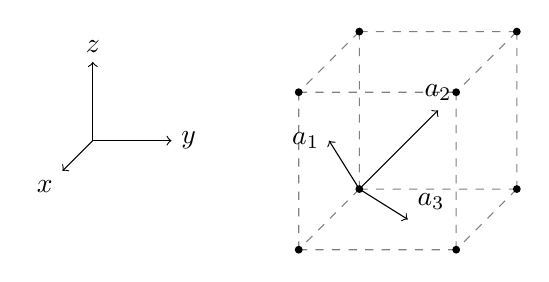
\begin{tikzpicture}
        \pgfmathsetmacro{\axissize}{1};
        \pgfmathsetmacro{\shiftx}{-4};
        \pgfmathsetmacro{\shifty}{0};
        \pgfmathsetmacro{\shiftz}{0};
        \draw[->] (\shiftx,\shifty, \shiftz) -- (\shiftx+\axissize,\shifty, \shiftz) node[right]{$y$};
        \draw[->] (\shiftx,\shifty, \shiftz) -- (\shiftx,\shifty+\axissize, \shiftz) node[above]{$z$};
        \draw[->] (\shiftx,\shifty, \shiftz) -- (\shiftx,\shifty, \shiftz+\axissize) node[below left]{$x$};
        \foreach \uda in {-1,+1}
        \foreach \udb in {-1,+1}
        \draw[gray, dashed]
        (-1,+\uda,+\udb) -- (+1,+\uda,+\udb)
        (+\uda,-1,+\udb) -- (+\uda,+1,+\udb)
        (+\uda,+\udb,-1) -- (+\uda,+\udb,+1)
        ;
        \foreach \x in {-1,+1}
        \foreach \y in {-1,+1}
        \foreach \z in {-1,+1}
        \draw[] (\x,\y,\z) node[fill=black, circle, inner sep=1pt]{};
        \draw[->] (-1,-1,-1) -- (-1,+0,+0) node[left]{$\ve a_1$};
        \draw[->] (-1,-1,-1) -- (+0,-1,+0) node[above right]{$\ve a_3$};
        \draw[->] (-1,-1,-1) -- (+0,+0,-1) node[above]{$\ve a_2$};
        \end{tikzpicture}
    \end{center}
    \[ \ve a_1 = \f{a}{2} \br{\hat y + \hat z} \quad \ve a_2 = \f{a}{2} \br{\hat x + \hat z} \quad \ve a_3 = \f{a}{2} \br{\hat x + \hat y} \]
    \item \term{Diamond Structure}: The diamond crystal structure consists of a fcc Bravais lattice with a $2$-atom basis,
    \begin{center}
        \begin{tikzpicture}[scale=2]
        \pgfmathsetmacro{\axissize}{0.5};
        \pgfmathsetmacro{\shiftx}{-3};
        \pgfmathsetmacro{\shifty}{0};
        \pgfmathsetmacro{\shiftz}{0};
        \draw[->] (\shiftx,\shifty, \shiftz) -- (\shiftx+\axissize,\shifty, \shiftz) node[right]{$y$};
        \draw[->] (\shiftx,\shifty, \shiftz) -- (\shiftx,\shifty+\axissize, \shiftz) node[above]{$z$};
        \draw[->] (\shiftx,\shifty, \shiftz) -- (\shiftx,\shifty, \shiftz+\axissize) node[below left]{$x$};
        \foreach \uda in {-1,+1}
        \foreach \udb in {-1,+1}
        \draw[gray, dashed]
        (-1,+\uda,+\udb) -- (+1,+\uda,+\udb)
        (+\uda,-1,+\udb) -- (+\uda,+1,+\udb)
        (+\uda,+\udb,-1) -- (+\uda,+\udb,+1)
        ;
        \foreach \x in {-1,+1}
        \foreach \y in {-1,+1}
        \foreach \z in {-1,+1}
        \draw[] (\x,\y,\z) node[fill=black, circle, inner sep=1pt]{};
        \draw[->] (-1,-1,-1) -- (-1,+0,+0) node[left]{$\ve a_1$};
        \draw[->] (-1,-1,-1) -- (+0,-1,+0) node[left]{$\ve a_3$};
        \draw[->] (-1,-1,-1) -- (+0,+0,-1) node[left]{$\ve a_2$};
        \draw[red, ->] (-1,+0,+0) -- ++ (0.6,0.6,0.6) node[above right]{$\ve r$};
        \draw[red, ->] (+0,-1,+0) -- ++ (0.6,0.6,0.6) node[above right]{$\ve r$};
        \draw[red, ->] (+0,+0,-1) -- ++ (0.6,0.6,0.6) node[above right]{$\ve r$};
        \end{tikzpicture}
    \end{center}
    \[ \hat r = \f{a}{4}\br{\hat x + \hat y + \hat z} \]
    \[ \ve a_1 = \f{a}{2} \br{\hat y + \hat z} \quad \ve a_2 = \f{a}{2} \br{\hat x + \hat z} \quad \ve a_3 = \f{a}{2} \br{\hat x + \hat y} \]
\end{enumerate}

The Diamond structure is a generalization of the graphene lattice in 3D. Many materials include C (diamond), Si, Ge and Sn crystallize in this diamond structure. The nearest-neighbor hopping Hamiltonian is as follows,
\[ H_1 = - \sum_{\ve R} \br{t \ket{\ve R, 1}\bra{\ve R, 2} + t \ket{\ve R + \ve a_1, 1}\bra{\ve R, 2} + t \ket{\ve R + \ve a_2, 1}\bra{\ve R, 2} + t \ket{\ve R + \ve a_3, 1} \bra{\ve R, 2} + \text{h.c.}} \eq \label{eq:diamond_H1}\]
While the second-nearest neighbor terms are numerous. In fact there are $24$ terms written below,
\begin{align*}
\eq \label{eq:diamond_H2}
\begin{split}
H_2
&= i \f{8 \De\tsb{SO}}{a^2} \sum_{\al \in \bc{1,2}}\sum_{\ve R} \bigg[\cdots \\
&\qquad \cdots + \ket{\ve R + \ve a_1,\al} \bra{\ve R, \al} \ve S \cdot \br{\ve r \times \ve a_1} + \cdots \\
&\qquad \cdots + \ket{\ve R + \ve a_2,\al} \bra{\ve R, \al} \ve S \cdot \br{\ve r \times \ve a_2} + \cdots \\
&\qquad \cdots + \ket{\ve R + \ve a_3,\al} \bra{\ve R, \al} \ve S \cdot \br{\ve r \times \ve a_3} + \cdots \\
&\qquad \cdots + \ket{\ve R + \ve a_2 - \ve a_1,\al} \bra{\ve R, \al} \ve S \cdot \br{\ve r - \ve a_1} \times \br{\ve r -\f{a}{2} \hat y} + \cdots \\
&\qquad \cdots + \ket{\ve R + \ve a_3 - \ve a_1,\al} \bra{\ve R, \al} \ve S \cdot \br{\ve r - \ve a_1} \times \br{\ve r -\f{a}{2} \hat z} + \cdots \\
&\qquad \cdots + \ket{\ve R + \ve a_2 - \ve a_3,\al} \bra{\ve R, \al} \ve S \cdot \br{\ve r - \ve a_3} \times \br{\ve r -\f{a}{2} \hat y} + \cdots \\
&\qquad \cdots + \text{h.c.} \bigg]
\end{split}
\end{align*}

We can explicitly calculate the cross products,
\begin{align*}
    \ve r \times \ve a_1 &= \f{a^2}{8}\br{\hat x + \hat y + \hat z} \times \br{\hat y + \hat z} = \f{a^2}{8} \br{\hat z - \hat y}\\
    \ve r \times \ve a_2 &= \f{a^2}{8}\br{\hat x + \hat y + \hat z} \times \br{\hat z + \hat x} = \f{a^2}{8} \br{\hat x - \hat z}\\
    \ve r \times \ve a_3 &= \f{a^2}{8}\br{\hat x + \hat y + \hat z} \times \br{\hat x + \hat y} = \f{a^2}{8} \br{\hat y - \hat x}\\
    \br{\ve r - \ve a_1} \times \br{\ve r - \f{a}{2} \hat y} &= \f{a^2}{16}\br{\hat x - \hat y - \hat z} \times \br{\hat x - \hat y + \hat z} = -\f{a^2}{8}\br{\hat x + \hat y} \\
    \br{\ve r - \ve a_1} \times \br{\ve r - \f{a}{2} \hat z} &= \f{a^2}{16}\br{\hat x - \hat y - \hat z} \times \br{\hat x + \hat y - \hat z} = +\f{a^2}{8}\br{\hat x + \hat z} \\
    \br{\ve r - \ve a_3} \times \br{\ve r - \f{a}{2} \hat y} &= \f{a^2}{16}\br{-\hat x - \hat y + \hat z} \times \br{\hat x - \hat y + \hat z} = +\f{a^2}{8}\br{\hat y + \hat z}
\end{align*}
Therefore \cref{eq:diamond_H2} becomes,
\begin{align*}
\eq \label{eq:diamond_H2_computed_cross_product}
\begin{split}
H_2
&= i \De\tsb{SO}\sum_{\al \in \bc{1,2}}\sum_{\ve R} \bigg[\cdots \\
&\qquad \cdots + \ket{\ve R + \ve a_1,\al} \bra{\ve R, \al} \br{S^z - S^y} + \cdots \\
&\qquad \cdots - \ket{\ve R + \ve a_2,\al} \bra{\ve R, \al} \br{-S^x + S^z} + \cdots \\
&\qquad \cdots + \ket{\ve R + \ve a_3,\al} \bra{\ve R, \al} \br{S^y - S^x} + \cdots \\
&\qquad \cdots - \ket{\ve R + \ve a_2 - \ve a_1,\al} \bra{\ve R, \al} \br{S^x + S^y} + \cdots \\
&\qquad \cdots + \ket{\ve R + \ve a_3 - \ve a_1,\al} \bra{\ve R, \al} \br{S^x + S^z} + \cdots \\
&\qquad \cdots + \ket{\ve R + \ve a_2 - \ve a_3,\al} \bra{\ve R, \al} \br{S^y + S^z} + \cdots \\
&\qquad \cdots + \text{h.c.} \bigg]
\end{split}
\end{align*}

The nearest neighbors Hamiltonian \cref{eq:diamond_H1} can be Fourier transformed and partially diagonalized,
\[ H_1 = - \sum_{\ve k}\bc{\ket{\ve k, 1}\bra{\ve k, 2} \br{\br{t + \de t} + t e^{-i \ve k \cdot \ve a_1} + t e^{-i\ve k\cdot \ve a_2} + t e^{-i\ve k \cdot \ve a_3}} + \text{h.c.}} \]
Similarly for \cref{eq:diamond_H2_computed_cross_product},

\begin{align*}
\eq \label{eq:diamond_H2_computed_cross_product_ft}
\begin{split}
H_2
&= i \De\tsb{SO}\sum_{\al \in \bc{1,2}}\sum_{\ve k} \ket{\ve k,\al} \bra{\ve k, \al} \bigg[\cdots \\
&\qquad \cdots + e^{-i \ve k \cdot \ve a_1} \br{S^z - S^y} + \cdots \\
&\qquad \cdots + e^{-i \ve k \cdot \ve a_2} \br{S^x - S^z} + \cdots \\
&\qquad \cdots + e^{-i \ve k \cdot \ve a_3} \br{S^y - S^x} + \cdots \\
&\qquad \cdots - e^{-i \ve k \cdot \br{\ve a_2 - \ve a_1}} \br{S^x + S^y} + \cdots \\
&\qquad \cdots + e^{-i \ve k \cdot \br{\ve a_3 - \ve a_1}} \br{S^x + S^z} + \cdots \\
&\qquad \cdots + e^{-i \ve k \cdot \br{\ve a_2 - \ve a_3}} \br{S^y + S^z} + \cdots \\
&\qquad \cdots + \text{h.c.} \bigg]
\end{split}
\end{align*}

Introducing pseudo-spin $\ve \si = \br{\si^x, \si^{y}, \si^{z}}$
\begin{align*}
\begin{split}
\si^x &= \begin{pmatrix} 0 & 1 \\ 1 & 0 \end{pmatrix} = \ket{1} \bra{2} + \ket{2} \bra{1} \\
\si^y &= \begin{pmatrix} 0 & -i \\ i & 0 \end{pmatrix} = -i\br{\ket{1} \bra{2} - \ket{2} \bra{1}} \\
\si^z &= \begin{pmatrix} 1 & 0 \\ 0 & -1 \end{pmatrix} = \ket{1} \bra{1} - \ket{2} \bra{2}
\end{split}
\end{align*}
The first and second nearest-neighbor Hamiltonian can be modeled when the tunneling amplitudes in \cref{eq:diamond_H1} are perturbed a small amount $t \mapsto t + \de t$ using the $5$-component vector $\ve d\br{\ve k} = \br{d_1\br{\ve k},d_2\br{\ve k},d_3\br{\ve k},d_4\br{\ve k},d_5\br{\ve k}}$,
\begin{align*}
    d_1\br{\ve k} &= - \br{t + \de t} - t \bs{\cos \ve k \cdot \ve a_1 + \cos \ve k \cdot \ve a_2 + \cos \ve k \cdot \ve a_3} \\
    d_2\br{\ve k} &= - t \bs{\sin \ve k \cdot \ve a_1 + \sin \ve k \cdot \ve a_2 + \sin \ve k \cdot \ve a_3} \\
    d_3\br{\ve k} &= \De\tsb{SO} \bs{\sin \ve k \cdot \ve a_2 - \sin \ve k \cdot \ve a_3 - \sin \ve k \cdot \br{\ve a_2 - \ve a_1} + \sin \ve k \cdot \br{\ve a_3 - \ve a_1}} \\
    d_4\br{\ve k} &= \De\tsb{SO} \bs{\sin \ve k \cdot \ve a_3 - \sin \ve k \cdot \ve a_1 + \sin \ve k \cdot \br{\ve a_1 - \ve a_2} - \sin \ve k \cdot \br{\ve a_3 - \ve a_2}} \\
    d_5\br{\ve k} &= \De\tsb{SO} \bs{\sin \ve k \cdot \ve a_1 - \sin \ve k \cdot \ve a_2 - \sin \ve k \cdot \br{\ve a_1 - \ve a_3} + \sin \ve k \cdot \br{\ve a_2 - \ve a_3}}
\end{align*}
Using this the full Hamiltonian can be written as,
\[ H\br{\ve k} = d_1\br{\ve k} \si^x + d_2\br{\ve k}  \si^y  + d_3\br{\ve k} \si^{z}S^x + d_4\br{\ve k} \si^z S^y + d_5\br{\ve k}\si^zS^z \]
Where the matrices on the right of each $d_i\br{\ve k}$ term are the usual $4 \time 4$ gamma matrices $\ga^{\mu}$ from the Dirac equation.
\[ \ga^{0} = \si^{x} \quad \ga^{0}\ga^{1} = \si^{y} \quad \ga^{0}\ga^{2} = \si^{z}S^{x} \quad \ga^{0}\ga^{3} = \si^{z}S^y \quad \ga^{0}\ga^{5} = \si^{z} S^{z}\]
\[ \ga^{1} = \si^{x} \si^{y} = i \si^z \quad \ga^{2} = i \si^{y}S^{x} \ga^{3} = i \si^{y}S^{y} \]
\[ i \ga^{0}\ga^{1}\ga^{2}\ga^{3} = i \si^{x} i \si^{z} i \si^{y}S^{x} = \si^{y}S^{z} \defined \ga^{5} \]
It is convenient to rename these matrices using capital gammas,
\begin{alignat*}{2}
\Ga^{1} &= \ga^{0} &= \si^{x} \\
\Ga^{2} &= \ga^{0}\ga^{1} &= \si^{y} \\
\Ga^{3} &= \ga^{0}\ga^{2} &= \si^{z}S^{x} \\
\Ga^{4} &= \ga^{0}\ga^{3} &= \si^{z}S^y \\
\Ga^{4} &= \ga^{0}\ga^{5} &= \si^{z} S^{z}
\end{alignat*}
It is easy to see that these $\Ga$ matrices obey the \term{Clifford Algebra},
\[ \bc{\Ga^{a}, \Ga^{b}} = 2 \de_{ab} \]
Thus we have that,
\[ H\br{\ve k} = \sum_{a = 1}^{5} d_a\br{\ve k}\Ga^{a} \defined d_a\br{\ve k}\Ga^{a} \eq \label{eq:HGa}\]
Just like in graphene, we see that the parity transformation $P = \si^{x} = \ga^{0}$ leaves $\Ga^{1}$ even under parity and $\Ga^{2,3,4,5}$ odd under parity. One reason motivating why we should write \cref{eq:HGa} in terms of the $\Ga$ matrices is that we can now easily find the eigenvalues by squaring the Hamiltonian,
\[ H^2\br{\ve k} = d_a\br{\ve k}\Ga^{a} d_b\br{\ve k}\Ga^{b} = d_a \br{\ve k} d_a\br{\ve k} \]
Therefore,
\[ \vep_{\pm}\br{\ve k} = \pm \sqrt{d_a \br{\ve k} d_a\br{\ve k}} = \pm \abs{\ve d\br{\ve k}} \]
We now elect to compute the reciprocal basis vectors. Recall that,
\[ \ve a_1 = \f{a}{2} \br{\hat y + \hat z} \quad \ve a_2 = \f{a}{2} \br{\hat x + \hat z} \quad \ve a_3 = \f{a}{2} \br{\hat x + \hat y} \]
Define the scalar $v_c$ such that,
\[ v_c = \ve a_1 \cdot \br{\ve a_2 \times \ve a_3} = \cdots = \f{a^3}{4} \]
The reciprocal vectors become,
\[ \ve b_1 = \f{2\pi}{v_c} \ve a_2 \times \ve a_3 = \f{2 \pi}{a} \br{\hat y - \hat x + \hat z} \]
Similarly,
\[ \ve b_2 = \f{2\pi}{v_c} \br{\hat z - \hat y + \hat x} \]
\[ \ve b_3 = \f{2\pi}{v_c} \br{\hat x - \hat z + \hat y} \]
Therefore the reciprocal lattice of fcc is the bcc lattice vectors and vice versa.
When $\de t = 0$ the $5$-component $\ve d\br{\ve k}$ vanishes at $3$ inequivalent band-touching point in the first Brillouin zone.
\[ X^{x} = \f{2\pi}{a}\br{1,0,0} \qquad X^{y} = \f{2\pi}{a}\br{0,1,0} \qquad X^{z} = \f{2\pi}{a}\br{0,0,1} \]
Considering the $X^{z}$ point as an illustrative example we have $k_1 = k_2 = \f12$ and $k_3 = 0$. If we expand in small deviations from the $X^z$ point where $\ve k \simeq X^{z} + \ve q = \br{q_x, q_y, \f{2\pi}{a} + q_z}$ we obtain the following,
\begin{align*}
    d_1\br{\ve k} &\simeq -t - \de t - t \br{-1} = - \de t \\
    d_2\br{\ve k} &\simeq t a q_z \\
    d_3\br{\ve k} &\simeq -2\De\tsb{SO} a q_x \\
    d_4\br{\ve k} &\simeq 2\De\tsb{SO} a q_y \\
    d_5\br{\ve k} &\simeq \f{\De\tsb{SO}}{8} a^3 \br{q_y^2 - q_x^2} q_z
\end{align*}
Thus we obtain (replacing $\ve q$ with $\ve k$ again),
\[ H_{X^{z}} = - \de t \si^{x} + t a k_z \si^{y} - 2 \De\tsb{SO} a \si^{z} S^{x} k_x + 2 \De\tsb{SO} a \si^{z} S^{y} k_y \]
Analogously expanding about $X^{y}$ and $X^{x}$,
\[ H_{X^{y}} = - \de t \si^{x} + t a k_y \si^{y} + 2 \De\tsb{SO} a k_x \si^{z} S^{x} - 2 \De\tsb{SO} a k_z \si^{z} S^{z} \]
\[ H_{X^{x}} = - \de t \si^{x} + t a k_x \si^{y} - 2 \De\tsb{SO} a k_y \si^{z} S^{y} + 2 \De\tsb{SO} a k_z \si^{z} S^{z} \]
Notice that $H_{X^{x,y,z}}$ look like anisotropic Dirac Hamiltonians where $\de t$ plays the role of the Dirac mass.
\[ \vep_{\pm}\br{\ve k} = \pm \sqrt{t^2 a^2 k_z^2 + 4 \De\tsb{SO}^2 a^2 \br{k_x^2 + k_y^2} + \de t^2} \]
Changing the sign of $\de t$ corresponds to transitions between topological and ordinary insulators.
\begin{itemize}
    \item $\de t > 0$: topological
    \item $\de t < 0$: ordinary
    \item $\de t = 0$: Dirac semimetal
\end{itemize}

\subsection{Quantum Hall Effect}

In this subsection we will discuss the Quantum Hall Effect. Specifically we will look at the Quantum Hall Effect in a $2$-dimensional electron gas (2DEG) when subjected to a magnetic field. 2DEG arise at heterointerfaces; interfaces between two different semiconductor materials. Semiconductors are insulators with a small band gap $<\SI{1}{\eV}$.

\begin{center}
\begin{tikzpicture}
    \draw (-3, 3) node[]{$\text{Al}_{x} \text{Ga}_{1-x} \text{As}$};
    \draw (+3, 3) node[]{$\text{GaAs}$};
    \draw (0, -3) -- (0, 3);
    \draw[dashed] (-4, 1) -- (+4, 1) node[right]{$\vep\tsb{F}$};
    \draw [] plot [smooth, tension=1] coordinates {(-4, 1.5) (-1, 1.8) (0, 2.5)};
    \draw [] plot [smooth, tension=1] coordinates {(+4, 1.5) (+1, 1.2) (0, 0.5)};
    \draw [] plot [smooth, tension=1] coordinates {(-4, -2.5) (-1, -2.2) (0, -1.5)};
    \draw [] plot [smooth, tension=1] coordinates {(+4, -0.5) (+1, -0.8) (0, -1.5)};
\end{tikzpicture}
\end{center}

Modeling a 2DEG corresponds to subjecting the electrons in state $\ket{\psi}$ to a potential $V\br{\ve r}$ and making use of the Schrödinger equation,
\[ \br{-\f{\hbar^2}{2m} \del^2 + V\br{\ve r}}\psi\br{\ve r} = E \psi\br{\ve r} \eq \label{eq:tise} \]
Where $\psi\br{\ve r} \defined \braket{\ve r}{\psi}$ is the position space wavefunction. In order to model electrons confined to two dimensions (say $x,y$) use the following potential,
\[ V\br{\ve r} = \begin{cases}
    0 & \ve r \cdot \hat z = 0 \\
    \inf & \ve r \cdot \hat z \neq 0
\end{cases} \eq \label{eq:potential}\]
By doing so, $\psi\br{\ve r}$ is confined to be non-zero within the $xy$-plane.
\[ \psi\br{\ve r} = \psi\br{x \hat x + y \hat y } \defined \psi\br{x,y} \]
Furthermore let $L_x$ and $L_y$ denote the side lengths of rectangle space accessible by the electrons equipped with periodic boundary conditions,
\[ \psi\br{x + L_x, y} = \psi\br{x, y+ L_y} = \psi\br{x,y} \eq \label{eq:boundary_conditions} \]
The electrons inside the accessible region are subject to no external potential. Therefore the electrons will exhibit plane-wave behaviour with $z = 0$.
\[ \psi\br{\ve r} = \ga e^{i \ve k \cdot \ve r} = \ga e^{i \br{k_x x + k_y y}} \eq \label{eq:2dansatz} \]
Where $\ve k = k_x \hat x + k_y \hat y$ denotes the momentum wave vector of the electron and $\ga \in \R$ is a normalization factor. The normalization factor comes from the desired normalization of the state $\psi\br{\ve r}$,
\[ 1 = \braket{\psi}{\psi} = \intl_{0}^{L_x} \dif x \intl_{0}^{L_y} \dif y \braket{\psi}{\ve r}\braket{\ve r}{\psi} = \intl_{0}^{L_x} \dif x \intl_{0}^{L_y} \dif y \ga^2 \abs{e^{i \br{k_x x + k_y y}}}^2 = L_x L_y \ga^2 \]
Therefore the normalization is simply,
\[ \ga = \f{1}{\sqrt{L_x L_y}} \]
Consequently \cref{eq:2dansatz} becomes,
\[ \psi\br{\ve r} = \f{1}{\sqrt{L_x L_y}} e^{i \br{k_x x + k_y y}} \]
Moreover the boundary conditions \cref{eq:boundary_conditions} quantize the accessible values of $k_x, k_y$,
\[ e^{i \br{k_x\br{x + L_x} + k_y y}} = e^{i \br{k_x x + k_y \br{y + L_y}}} = e^{i \br{k_x x + k_y y}} \]
\[ e^{i k_x L_x} = e^{i k_y L_y} = 1 \implies k_x = \f{2 \pi m_x}{L_x} \quad k_y = \f{2 \pi m_y}{L_y} \quad m_x, m_y \in \bc{0, \pm 1, \pm 2,\ldots} \]
Therefore the accessible points in $k$-space form a square lattice which is illustrated below,
\begin{center}
    \begin{tikzpicture}
        \pgfmathsetmacro{\plotsize}{4};
        \pgfmathsetmacro{\ll}{0.6};
        \pgfmathsetmacro{\count}{5};
        \pgfmathsetmacro{\shift}{0.3};

        \draw[thick, ->] (-\plotsize, +0) -- (+\plotsize, +0) node[right]{$k_x$};
        \draw[thick, ->] (+0, -\plotsize) -- (+0, +\plotsize) node[above]{$k_y$};

        \foreach \x in {-\count,...,\count}{
            \foreach \y in {-\count,...,\count}{
                \draw (\ll*\x, \ll*\y) node[circle, inner sep=1pt, fill=red](\x d \y){};
            }
        }

        \draw[|<->|] ($\ll*(-5,-5) + (0,-\shift)$) -- node[below]{$\f{2\pi}{L_x}$} ($\ll*(-4,-5) + (0,-\shift)$);
        \draw[|<->|] ($\ll*(-5,-5) + (-\shift,0)$) -- node[left ]{$\f{2\pi}{L_y}$} ($\ll*(-5,-4) + (-\shift,0)$);

        \draw[blue, fill=blue, fill opacity=0.2] (3*\ll,3*\ll) +(-\ll/2,-\ll/2) rectangle +(+\ll/2,+\ll/2);
        \draw[green, fill=green, fill opacity=0.2] (0,0) circle (2);
        \draw[->] (0,0) -- node[below]{$k$} ({sqrt(2)},{sqrt(2)});
    \end{tikzpicture}
\end{center}
Clearly, each accessible momentum state occupies an area (shaded in blue) equal to,
\[ \br{\f{2\pi}{L_x}}\br{\f{2\pi}{L_y}} = \f{\br{2 \pi}^2}{\s A} \]
Where $\s A = L_x L_y$ is the total area. In the inverse of this statement is that there are,
\[ \f{\s A}{\br{2\pi}^2} \eq \label{eq:area}\]
grid points per unit area of $k$-space. Using \cref{eq:tise}, we can now calculate the energy for the state $\psi\br{r_x, r_y} \defined \braket{\ve r}{\psi}$.
\[ E \psi \br{\ve r} = -\f{\hbar^2}{2m} \del^2 \psi\br{\ve r} = -\f{\hbar^2}{2m} \br{\di_x^2 + \di_y^2} \psi\br{\ve r} = -\f{\hbar^2}{2m} \br{-k_x^2 -k_y^2} \psi\br{\ve r} = \f{\hbar^2}{2m} k^2 \psi\br{\ve r}\]
Where $k = \sqrt{k_x^2 + k_y^2}$ is a radius in $k$-space. Therefore the energy levels are,
\[ E = \f{\hbar^2 k^2}{2m} = \f{\hbar^2}{2m}\br{2\pi}^2 \br{\f{m_x^2}{L_x^2} + \f{m_y^2}{L_y^2}} \qquad m_x, m_y \in \bc{0, \pm1, \pm2, \ldots} \eq \label{eq:energy_levels}\]
Let $N\br{\vep}$ denote the number of states accessible to a single electron with energy $\vep$. Since this function is generally non-trivial, we approximate $N\br{\vep}$ as the infinitesimal amount $\de N\br{\vep}$ as follows,
\[ \de N\br{\vep} \simeq N_{<} \br{\vep + \de \vep/2} - N_{<} \br{\vep - \de \vep/2} \]
Where $N_{<}\br{\vep}$ is the number of states accessible to any electron with at most energy $\vep$. Evidently this quantity is proportional to an area in $k$-space. Namely, the area of $k$ space associated with $N_{<}$ is a circle centered at $\br{k_x, k_y} = \br{0,0}$. Therefore,
\[ N_{<}\br{\vep} \propto \pi k^2 = \pi \f{2m \vep}{\hbar^2} \]
The proportionality constant is exactly \cref{eq:area},
\[ N_{<}\br{\vep} = \f{\s A}{\br{2\pi}^2} \f{2m\pi  \vep}{\hbar^2} \]
Therefore,
\[ \de N\br{\vep} = \f{\s A}{\br{2\pi}^2} \f{2m\pi}{\hbar^2} \de \vep \]
Forming a differential form,
\[ \der{N}{\vep} = \f{\s A}{\br{2\pi}^2} \f{2m\pi}{\hbar^2} \]
The density of states is a constant. Normalizing for area,
\[ \f{1}{\s A}\der{N}{\vep} = \f{2m\pi}{\br{2\pi}^2\hbar^2} \]
This however, does not account for the fact that each electron has two accessible spin states for each $k$-space lattice point. Therefore, there are truly twice as many states available to each electron,
\[ \f{1}{\s A}\der{N}{\vep} = \f{4m\pi}{\br{2\pi}^2\hbar^2} \]
Therefore the density of states is,
\[ g\br{\vep} \defined \f{1}{\s A}\der{N}{\vep} = \f{m}{\pi \hbar^2} \eq \label{eq:2d_density_of_states} \]
The electron density for a given Fermi wavevector $k\tsb{F}$ is the number of electrons per unit area in $r$-space. At zero temperature and Fermi energy $\vep\tsb{F}$ the states in $k$-space are occupied at lowest energies first. Therefore the total number of electrons $N\br{\vep\tsb{F}}$ is given by,
\[ N\br{\vep\tsb{F}} = \s A\int_{0}^{\vep\tsb{F}} \dif \vep g\br{\vep} = \s A \int_{0}^{\vep\tsb{F}} \dif \vep \f{m}{\pi \hbar^2} = \f{m}{\pi \hbar^2} \vep\tsb{F} \s A \]
Given that the Fermi energy and Fermi wavevector are related via \cref{eq:energy_levels}, the electron density is,
\[ n\br{k\tsb{F}} = \f{1}{\s A} N\br{k\tsb{F}} = \f{m}{\pi \hbar^2} \f{\hbar^2 k\tsb{F}^2}{2m} \]
\[ n\br{k\tsb{F}} = \f{k\tsb{F}^2}{2\pi} \eq \label{eq:electron_density}\]

Now, we place the 2DEG in the $xy$-plane and subject it to a magnetic field in the $z$-direction $\ve B = B \hat z$. If the electrons are classical particles of charge $-e$ and mass $m$,
\[ \der{\ve p}{t} = \ve F\tsb{L} = - \f{e}{c}\ve v \times \ve B \qquad \ve v = \f{\ve p}{m}, \ve v = \der{\ve r}{t} \]
Solving these equations yields,
\[ m \dder{\ve r}{t} = - \f{e}{c} \der{\ve r}{t} \times \ve B  \]
Therefore we obtain a two dimensional system of coupled ordinary differentiable equations,
\begin{align*}
\dder{x}{t} &= - \f{eB}{mc} \der{y}{t} \\
\dder{y}{t} &= \f{eB}{mc} \der{x}{t}
\end{align*}
Where the frequency $\w_c = \f{eB}{mc}$ is the cyclotron frequency. In order to solve this system, introduce a complex parameter $z = x + i y$ such that,
\[ \dder{x}{t} = i \w_x \der{z}{t} \]
\[ z\br{t} = z_0 - \f{i v_0}{\w_c}e^{i \w_c t}  \]
Which is circular motion with frequency $\w_c$. Therefore if we need to model the average time between collisions with impurities, the simplest description involves a decrease in momentum with characteristic time $\tau$.
\[ \der{\ve p}{t} = - e \br{\ve E + \f{1}{c} \ve v \times \ve B} - \f{\ve p}{\tau} \]
Therefore without a magnetic field we have,
\[ \der{\ve p}{t} = \f{- \ve p}{t} \implies \ve p\br{t} = \ve p\br{0} e^{- t/\tau} \]
In general,
\[ m\der{\ve v}{t} = - \f{m \ve v}{\tau} - e\br{\ve E + \f{1}{c} \ve v \times \ve B} \]
Assuming that $\ve E$ and $\ve B$ are time-independent, we can look for the time-independent steady state solution corresponds to a fixed $\ve v$,
\[ \der{\ve v}{t} = 0 \implies \ve v = -\f{e \tau}{m} \br{\ve E + \f{1}{c} \ve v \times \ve B} \]
The electron $\ve v$ is connect to the current density $\ve j$ through the following equation we have seen before,
\[ \ve j = - e n \ve v \]
Where $n$ is the electron density and $e$ is the electric charge. Therefore,
\[ \ve j = \f{e^2 n \tau}{m} \br{\ve E - \f{e \tau}{m c} \ve j \times \ve B} \]
In the absence of a magnetic field $\ve B$, we recover Ohm's law,
\[ \ve j = \f{e^2 n \tau}{m} \ve E \]
Where the proportionality is the conductivity $\si$,
\[ \si = \f{e^2 n \tau}{m} \]
The electric field is,
\[ \ve E = \f{\ve j}{\si} = \f{1}{nec} \ve B \times \ve j \]
Component-wise,
\begin{align*}
    E_x &= \f{1}{\si} j_x + \f{B}{nec} j_y \\
    E_y &= \f{1}{\si} j_y - \f{B}{nec} j_x
\end{align*}
If there is no current in the $y$-direction ($j_y = 0$) we have,
\[ E_y = -\f{B}{nec} j_x \qquad \f{E_y}{B j_x} = -\f{1}{nec} = - R_H \]
The last equality is a definition of the \term{Hall coefficient} $R_H$
\[ R_H = \f{1}{nec} \]
Notice that the Hall coefficient only depends on the density of the electrons and other fundamental constants. Now we introduce the \term{resistivity tensor},
\[\rho = \begin{pmatrix}
    1 / \si & B R_{H} \\
    -B R_{H} & 1 / \si \\
\end{pmatrix} \]
We refer to this as the \term{classical Hall effect}.

\begin{center}
\begin{tikzpicture}
    \pgfmathsetmacro{\axissize}{4};
    \pgfmathsetmacro{\plotsize}{4};
    \draw[->] (0,0) -- (+\axissize,0) node[right]{$B$};
    \draw[->] (0, 0) -- (0,+\axissize) node[above]{$\rho_{xy}$};
    \draw[red] (1, 0) arc (0:27:1) node[midway, right]{$R_{H}$};
    \draw[scale=1.0,domain=0:\plotsize,smooth,variable=\B,red] plot ({\B},{0.5*\B});
\end{tikzpicture}
\end{center}

In reality, the classical Gall effect occurs at weak magnetic fields or in dirty samples.
If we let $1/\tau$ characterize the impurity scattering rate, our classical Hall effect is relevant in the domain where,
\[ \w_{C} \tau \ll 1 \]
Recall that the cyclotron frequency is $\w_c$,
\[ \w_c = \f{eB}{mc} \]
If $\w_{C} \tau \ll 1$, the electron will be scatter many times before being able to complete a single circular orbit; i.e. if the period of the circular motion of the electron is greater than the mean-free time, then we can model the electrons as a classical particle.\\

In we have $\w_{C} \tau \gg 1$, then the classical Hall effect is no longer the dominant feature. If the circular motion of the electrons becomes quantized, we need to consider the \term{quantum Hall effect}. The quantum aspects of the electron need to be considered in really clean materials or in high magnetic fields.\\

To study the quantum Hall effect, consider free quantum particles of charge $-e$ in the $xy$-plane in a magnetic field $\ve B= B \hat z$ pointing in the $\hat z$ direction. In the absence of a magnetic field, we have the relation $\ve p = m \ve v$ which makes the Hamiltonian,
\[  H = - \f{\hbar^2 \del^2}{2m} \]
However, a magnetic field $\ve B = \vdel \times \ve A$ we have,
\[ m \ve v = \ve p + \f{e}{c} \ve A \]
Therefore the Hamiltonian for a charged particle in a magnetic field is,
\[ H = \f{1}{2m} \br{- i \hbar \vdel + \f{e}{c} \ve A}^2 - \ve \mu \cdot \ve B \]
Where $\ve \mu$ is the magnetic dipole moment. For simplicity, we neglect $\ve \mu$ for now. Therefore, the Hamiltonian of interest is,
\[ H = \f{1}{2m} \br{- i \hbar \vdel + \f{e}{c} \ve A}^2 \eq \label{eq:quantum_hall_ham} \]
Where we wish to find the energy eigenstates $\psi$ where $H \psi = E \psi$. Moreover, the magnetic field is determined by $\ve B = \vdel \times \ve A$ leaving a \term{gauge invariance} in the choice of $\ve A$,
\[ \ve A \to \ve A + \vdel f \]
The gauge choice we will used is called the \term{Landau gauge}.
\[ \ve A = x B \hat y \]
Therefore,
\[ \br{\vdel \times \ve A}_{z} = \pder{A_y}{x} - \pder{A_x}{y} = B \]
Analogously the $x,y$ components of $\vdel \times \ve A$ are as follows,
\[ \br{\vdel \times \ve A}_{x} = \pder{A_z}{y} - \pder{A_y}{z} = 0 \]
\[ \br{\vdel \times \ve A}_{y} = \pder{A_x}{z} - \pder{A_z}{x} = 0 \]
Therefore \cref{eq:quantum_hall_ham} becomes,
\begin{align*}
    H
    &= \f{1}{2m}\br{- i \hbar \vdel + \f{e}{c} \ve A}^2 \\
    &= \f{1}{2m}\br{- i \hbar \vdel + \f{e\ve B}{c} \times \hat y}^2 \\
    &= - \f{\hbar^2}{2m} \pdder{}{x} + \f{1}{2m}\br{- i \hbar \pder{}{y} + \f{eB}{c}x}^2 \eq \label{eq:quantum_hall_ham_landau}
\end{align*}
Notice that $H$ is not invariant with respect to translations along the $x$-direction but \textit{is} invariant with respect to translations along the $y$-direction. Translation symmetries give rise to wave functions that are also momentum eigenstates. If the energy eigenstates $\psi\br{x,y}$ are thus functions of $x,y$ and have the following form,
\[ H \psi\br{x,y} = E \psi\br{x,y} \]
Symmetry analysis suggests we should expect $\psi$ to the separable into a plane wave solution with non-trivial $x$-dependence $\varphi\br{x}$.
\[ \psi\br{x,y} = e^{i k_y y} \varphi\br{x} \]
With $k_y$ to be determined. Substituting this ansatz into \cref{eq:quantum_hall_ham_landau} yields,
\[ E \psi\br{x,y}= - \f{\hbar^2}{2m} \pdder{\varphi}{x} e^{ik_yy} + \f{1}{2m}\br{\hbar k_y + \f{eB}{c}x}^2 \varphi e^{ik_yy} \]
Canceling $\varphi$,
\[ E \varphi = - \f{\hbar^2}{2m} \pdder{\varphi}{x} + \f{1}{2m}\br{\hbar k_y + \f{eB}{c}x}^2 \varphi \eq \label{eq:hall1D}\]
Gives us a 1D differential equation. For convenience of notation we introduce the \term{magnetic length} $\ell$,
\[ \ell = \sqrt{\f{\hbar c}{eB}} \]
Additionally re-use the classical cyclotron frequency,
\[ \w_{C} = \f{eB}{mc} \]
Using these constants, \cref{eq:hall1D} can we re-expressed as,
\[ -\f{\hbar^2}{2m} \pdder{\varphi}{x} + \f{m\w_{C}^2}{2} \br{x + k_y \ell^{2}}^2 \varphi = E \varphi \]
At this stage, it should be clear that this Hamiltonian is nothing more than a 1D Harmonic oscillator with frequency $\w_{C}$ and centered at $x = - k_y \ell^{2}$. The solution for the quantum harmonic oscillator can be found in a number of undergraduate quantum theory textbooks.
\[ \psi_{n k_y}\br{x} = \f{e^{ik_y y}}{\sqrt{\ell \sqrt{\pi} 2^{n} n!}} e^{-\f{1}{2 \ell^2} \br{x + k_y \ell^2}^2} H_n\br{\f{x + k_y \ell^2}{\ell}} \]
Where $H_n$ is the \term{$n$-th Hermite polynomial}. The wave function solutions are given by the Hermite polynomials, but the important feature are the quantized energy levels,
\[ E_{n,k_y} = \hbar \w_c \br{n + \f12} \qquad n \in \bc{0, 1, 2, \ldots} \]
Where $n$ are referred to as the Landau levels. This energy level is completely independent of $k_y$ but $k_y$ is independently quantized like a particle in a periodic potential,
\[ k_y = \f{2\pi}{L_y} m_y \qquad m_y \in \bc{0, \pm 1, \pm 2, \ldots}\]
Since the effective harmonic oscillator is centered at $-k_y \ell^2$, it must be that $L_x$ is twice the position of $k_y \ell^2$,
\[ -L_x \leq -k_y \ell^2 \leq 0 \implies 0 \leq k_y \leq \f{L_x}{\ell^2} \]
Therefore the total number of states for a fixed Landau level $n \in \bc{0,1,2,\ldots}$ is given by the $m_y$ value such that $k_y$ is bounded by $L_x / \ell^2$,
\[ N_{\phi} = \max{m_y} = \max{k_y} \f{L_y}{2\pi} = \f{L_yL_x}{2\pi\ell^2} = \f{L_xL_y eB}{2 \pi \hbar c}  \eq \label{eq:landau_occupancy}\]
Which is independent of $n$. Therefore, the number of electrons in each Landau level is the same for each Landau level. The density of states $g\br{\vep}$ forms a Dirac comb structure. In reality, however, the uncertainty principle smooths this plot due to uncertainty broadening. For low scattering rates (pure materials) we have the following profile.
\begin{center}
    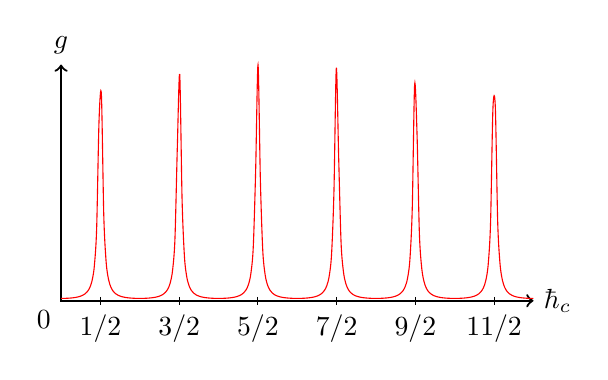
\begin{tikzpicture}
        \draw[thick, <->] (0, 3) node[above]{$g\br{\vep}$} -- (0,0) node[below left]{$0$} -- (6,0) node[right]{$\f{\vep}{\hbar \w_c}$};
        \draw[red, samples=200,smooth, domain=0:6, variable=\e] plot ({\e}, {0.03/((cos(deg(pi*\e)))^2 + 0.01)});
        \foreach \x in {1,3,5,7,9,11}{
            \draw ({\x/8*4}, +0.05) -- ({\x/8*4}, -0.05) node[below]{$\x/2$};
        }
    \end{tikzpicture}
\end{center}
Broadening increases due to impurities for the following reason. Suppose that an electron exists in a quantum state for some time $\tau$ which corresponds to the mean free time between collisions. The uncertainty in energy time is,
\[ \De \vep \De t \sim \De \vep \tau \sim \hbar \implies \De \vep \sim \f{\hbar}{\tau} \]
In regimes where $\tau$ is very small, the broadening results in the following,
\begin{center}
    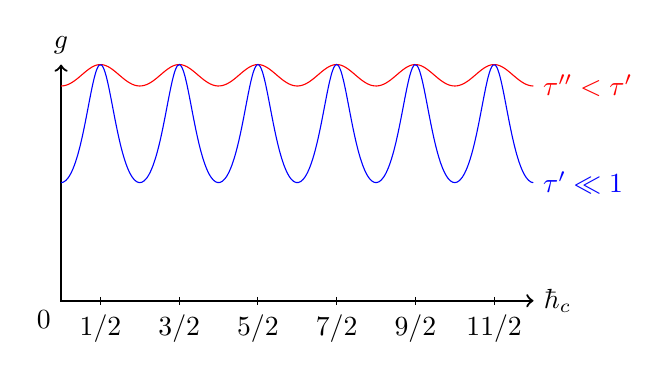
\begin{tikzpicture}
        \draw[thick, <->] (0, 3) node[above]{$g\br{\vep}$} -- (0,0) node[below left]{$0$} -- (6,0) node[right]{$\f{\vep}{\hbar \w_c}$};
        \draw[red, samples=200,smooth, domain=0:6, variable=\e] plot ({\e}, {30/((cos(deg(pi*\e)))^2 + 10)})node[right]{$\tau'' < \tau'$};
        \draw[blue, samples=200,smooth, domain=0:6, variable=\e] plot ({\e}, {3/((cos(deg(pi*\e)))^2 + 1)}) node[right]{$\tau' \ll 1$};
        \foreach \x in {1,3,5,7,9,11}{
            \draw ({\x/8*4}, +0.05) -- ({\x/8*4}, -0.05) node[below]{$\x/2$};
        }
    \end{tikzpicture}
\end{center}
Which more closely approximates the classical regime when $\w_c \tau \ll 1$ and the density $g\br{\vep}$ becomes more uniform.
\[ g\br{\vep} \approx g_0 = \f{m}{\pi \hbar^2} \]
Which is identically the 2D electron density of states in the absence of a magnetic field \cref{eq:2d_density_of_states}.\\

We refer to these energy levels as \term{Landau levels}. Every Landau level is degenerate with respect to all the different values of $k$. Since $E_{nk}$ is independent of $k$, we say that $E_{nk}$ has degeneracies in $k$. Because of this, Landau levels are analogous to bands in a crystal. \\

An alternative interpretation of \cref{eq:landau_occupancy} is to define the following: The total magnetic flux through the sample area $B L_x L_ y \defined \phi$ and the magnetic flux quantum $hc / e \defined \phi_0$. Then the Landau occupancy number becomes a flux ratio,
\[ N_{\phi} = \f{\phi}{\phi_0} \]

Combining the Landau level description at high magnetic fields $B$ gives a completely new description of the resistivity $\rho_{xy}$ and $\rho_{xx}$,

\begin{center}
    \hspace*{+3em}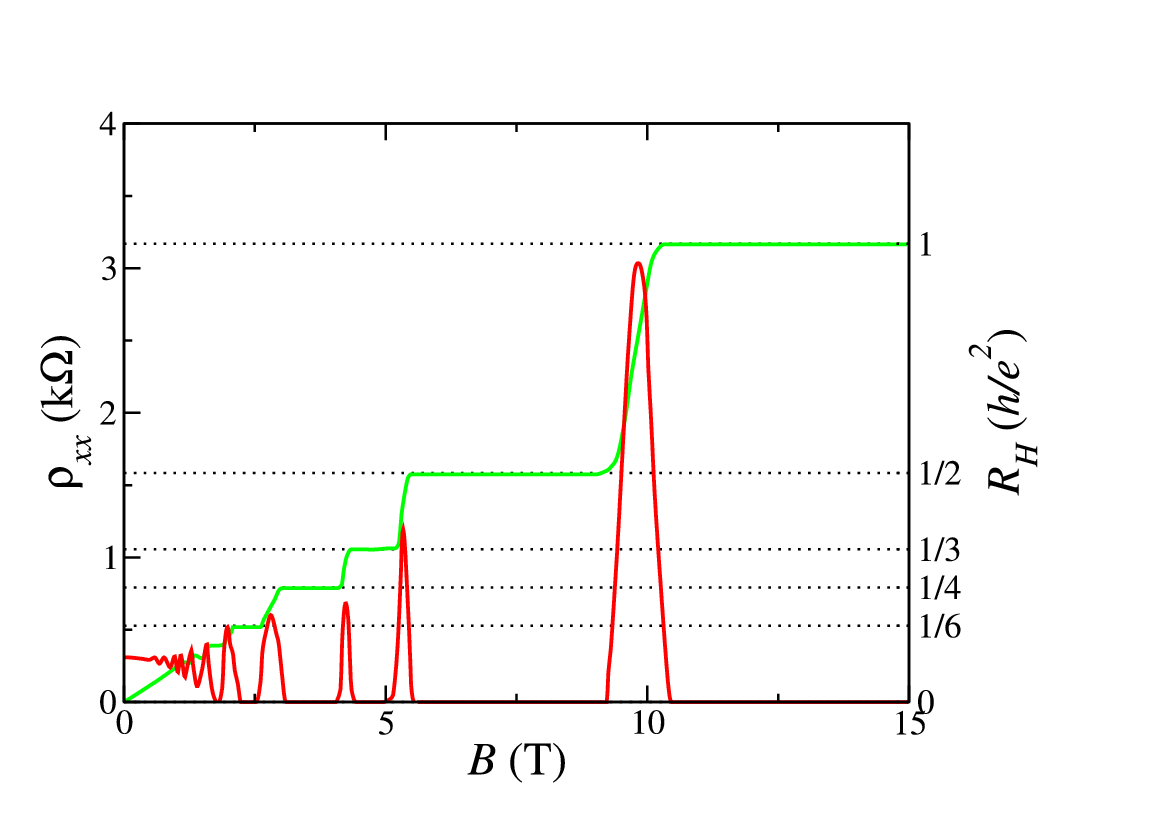
\includegraphics[width=\textwidth]{figures/quantum_hall_effect.png}
\end{center}

It can be seen that $\rho_{xy}$ develops perfectly flat plateaus exactly when $\rho_{xy} = h / e^2 \nu$ where $\nu$ is an integer (this is why we refer to this phenomena as the \term{integer quantum hall effect}; this contrasts the \term{fractional quantum hall effect} where $\nu$ is permitted to be any fraction). In fact $\nu$ is called the integer Landau level filling factor corresponding to the number of completely filled Landau levels. \\

The states at the center of each Landau level are delocalized and can contribute to transport. States in the tails of each Landau level are localized and can not contribute to transport. When considering $k_B T \ll \hbar c$, the temperature of the system can be treated as effectively zero. In these cases, the Fermi-Dirac distribution $f\br{\vep}$
\[ f\br{\vep} = \f{1}{e^{\br{\vep - \mu}/kT} + 1} \]
Tends towards the following step function,
\[ \lim_{T \to 0} f\br{\vep} = \begin{cases}
    1 & \vep < \mu \\
    0 & \vep > \mu
\end{cases} \]
At this temperature scale, the chemical potential is effectively the the Fermi energy $\vep\tsb{F}$. This makes sense; the typically energy $\mu$ to add/remove an electron would be the equivalent to the edge state fermions $\vep\tsb{F}$. As the magnetic field increases the Landau occupancy $N_{\phi}$ increases letting $\vep\tsb{F}$ tend to zero at higher and higher energies. For a fixed total number of particles $N$,
\[ \nu = \left\lfloor{\f{N}{N_{\phi}}}\right\rfloor \eq \label{eq:nu}\]
Gives the total number of \textit{completely} filled Landau levels while the Fermi energy $\vep\tsb{F}$ is simply the energy of the maximal Landau level that is at least partially occupied.
\[ \vep\tsb{F} = E_{\nu + 1} = \hbar \w_c \br{\nu + \f32} \eq \label{eq:fermi} \]
Therefore $\vep\tsb{F} = \mu$ becomes a function of $B$ for fixed $N$,
\[ \mu\br{B} = \hbar \f{e B}{mc} \br{\left\lfloor{\f{N{2 \pi \hbar c}}{{L_xL_y eB}}}\right\rfloor + \f12} \]
For fixed $N$ as $B \to \inf$, the floor function eventually reaches zero and the chemical potential tends as a straight line with slope $\f{\hbar e}{2mc}$. In order to plot this function consider setting $\hbar = c = e = m = 1$ and defining fixed $\ti n = 2 \pi N / (L_xL_y)$,
\[ \mu\br{B} = B \br{\left\lfloor{\f{\ti n}{B}}\right\rfloor + \f32} \]
\begin{center}
    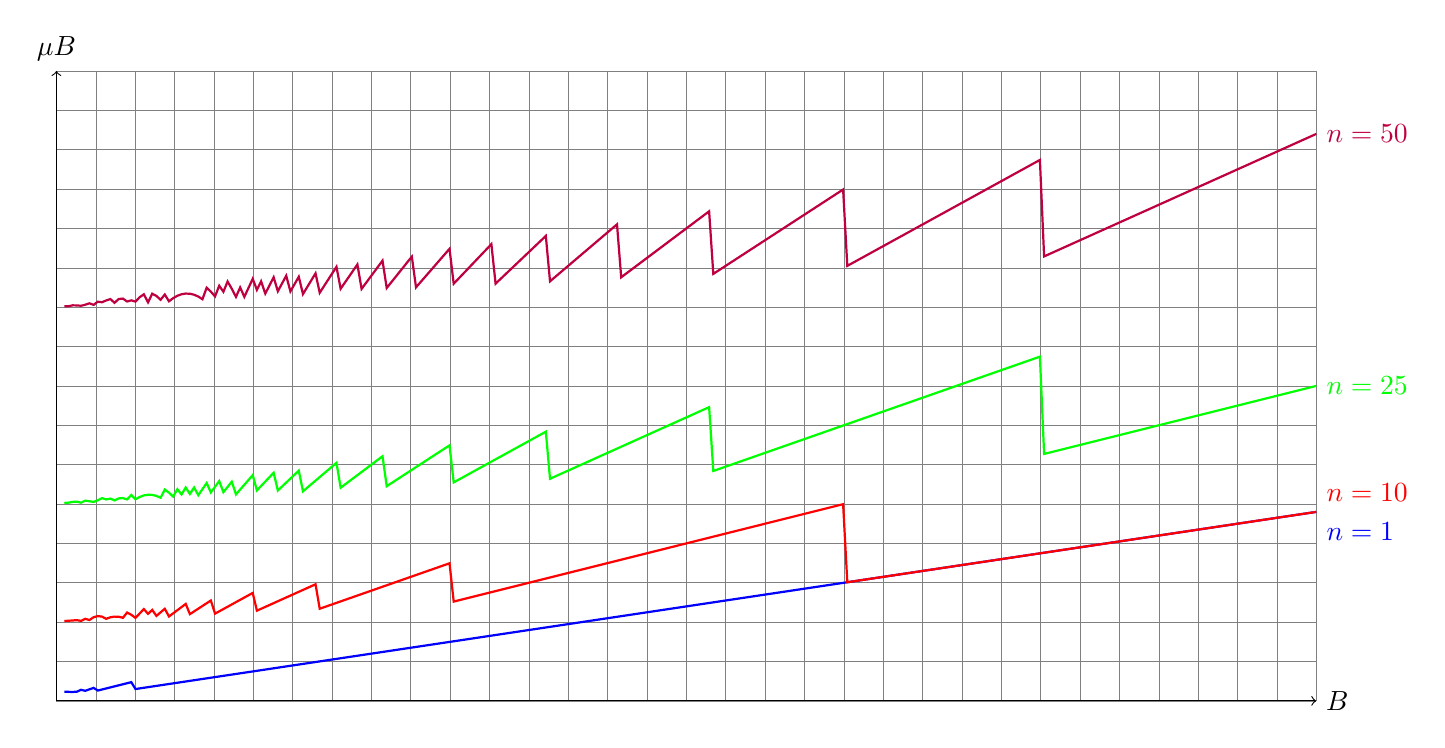
\begin{tikzpicture}
        \draw[step=.5cm,gray,very thin] (0,0) grid (16,8);
        % \draw[red, thick, domain=0:8, samples=300] plot (\x, {floor(\x)}) node[right] {$\lfloor x \rfloor$};
        % \draw[black,  thick, domain=0:8] plot(\x, \x) node[right] {$x$};
        % \draw[black, thick, domain=0:8] plot(\x, \x/2) node[right] {$x/2$};
        \draw[blue  , thick, domain=0.1:16, samples=300] plot(\x, {0.1*\x*(floor(( 1/\x)) + 3/2)})  node[below right] {$\ti n = 1$};
        \draw[red   , thick, domain=0.1:16, samples=300] plot(\x, {0.1*\x*(floor((10/\x)) + 3/2)})  node[above right] {$\ti n = 10$};
        \draw[green , thick, domain=0.1:16, samples=300] plot(\x, {0.1*\x*(floor((25/\x)) + 3/2)})  node[right] {$\ti n = 25$};
        \draw[purple, thick, domain=0.1:16, samples=300] plot(\x, {0.1*\x*(floor((50/\x)) + 3/2)})  node[right] {$\ti n = 50$};
        \draw [<->] (0,8) node[above]{$\mu\br{B}$} -- (0,0) -- (16,0) node[right]{$B$};
    \end{tikzpicture}
\end{center}

As the magnetic field increases, $N_{\phi} \propto B$ increases and $\vep\tsb{F}$ moves towards zero through the Landau levels. When $\vep\tsb{F}$ is in the mobility gap, the system behaves like an insulator while when it passes through the Landau level centers, it becomes metallic. This explains why nothing changes at the plateaus of $\rho_{xy}$ but doesn't explain why $\rho_{xy}$ is non-zero and quantized to precise values. This has to do with the existence of edge states. Consider a sample 2DEG that is finite in the $x$-direction admitting zero potential in regions between $\pm L_x / 2$ but approaches an infinite barrier at $V\br{\pm L_x / 2} = \inf$. Then the Schrödinger equation yields the familiar shifted harmonic oscillator with potential $V\br{x}$,
\[ \f{\hbar^2}{2m} \dder{\varphi}{x} + \f{m\w_c^2}{2}\br{x + k_y \ell^2} \varphi + V\br{x} \varphi = E \varphi \]
At $V = 0$, $\varphi \sim e^{-\f{1}{2\ell^2}\br{x+k_y\ell^2}^2}$ varies on the scale of the magnetic length $\ell$. Suppose that $V\br{x}$ is very slowly varying on this scale. In this limit, we can solve the Schrödinger equation by simply replacing $V\br{x} \approx V\br{k_y \ell^2}$. The eigenvalues then become,
\[ E_{nk_y} = \hbar \w_c \br{n + \f12} + V\br{k_y \ell^2} \]
Thus when $\vep\tsb{F}$ is between the Landau levels in the bulk, there are still states at the Fermi energy of the edges of the system (called the edge states). Their number is equal to the number of filled Landau levels (edges are populated for each Landau level last). Moreover, near the intersection with $\vep\tsb{F}$ the dispersion is \textit{chiral},
\[ E_{n k_y} \simeq \vep\tsb{F}\pm\hbar v_n \br{k_y \pm k_{y,n}} \]
As we have seen before in \cref{eq:chrial_dispersion}, the existence of the chiral edge states implies the Hall effect,
\[ I_y = -e \int \f{\dif k}{2 \pi} v n\tsb{F}\br{\vep_k} \]
Since $\dif k = \dif \vep / \hbar v$,
\[ I_R = - \f{e}{2\pi \hbar}\int_{-\inf}^{\vep\tsb{FR}} \dif \vep n\tsb{F}\br{\vep} \]
\[ I_L = - \f{e}{2\pi \hbar}\int_{-\inf}^{\vep\tsb{FL}} \dif \vep n\tsb{F}\br{\vep} \]
Therefore,
\[ I_y = I_R + I_L = -\f{e}{h} \br{\vep\tsb{FR} - \vep\tsb{FL}} = -\f{e^2}{h}V_x \]
Such each filled Landau level contributes $\si_{yx} = - e^2 / h$ to the total Hall conductivity. Using the Landau level filling factor $\nu$,
\[ \si_{yx} = - \f{e^2}{h} \nu \]
Analogously,
\[ \si_{xy} = + \f{e^2}{h} \nu \]
As long as $\vep\tsb{F}$ is in the \textit{mobility gap} between Landau levels, $\si_{xy}$ stays pinned at this value since the number of edge states doesn't change and the bulk states don't contribute. Therefore,
\[ \si = \begin{pmatrix}
    0 & + \f{e^2}{h}\nu \\
    - \f{e^2}{h}\nu & 0 \\
\end{pmatrix} \]
The resistivity tensor is defined such that,
\[ \rho_{xx} = \f{\si_{xx}}{\si_{xx}^2 + \si_{xy}^2} = 0 \]
\[ \rho_{xy} = -\f{\si_{xy}}{\si_{xx}^2 +\si_{xy}^2} = - \f{1}{\si^{xy}} = - \f{h}{e^2} \nu \]
Amazingly, $\rho_{xx}$ and $\si_{xx}$ are zero simultaneously. Therefore a 2DEG in the quantum Hall regime behaves both as perfect insulator and a perfect conductor (in the appropriate directions).

\subsubsection{Conclusion}

The topological features of electronic structures we have considered thus far are genuine manifestations of quantum mechanics on macroscopic scales. For example, resistivity in the Quantum Hall effect,
\[ \rho_{xy} = \f{h}{e^2 \nu} \]
Has dependence on Planck's constant $h$ which indicates that it has no classical counterpart. This is in contrast with the Classical Hall effect,
\[ \rho_{xy} = \f{B}{nec} \]
which does not rely on quantum mechanics whatsoever. This concludes the first focus of this course and one of the major ideas in condensed matter physics: the effects of the electronic structure topology on macroscopic scales. \\

\section{Electron-electron Interactions}

Heretofore, we have consider materials where electrons are modeled as moving in a atomic lattice in \textit{isolation}. In essence, the electrons are treated as being non-interacting. This approximation was well-founded as many material properties can be seen as consequences of non-interacting electrons and in most cases, electron interactions are negligible. \\

However, in specific cases the electron interactions yield interesting physics. For example Landau Fermi liquid theory, magnetism and superconductivity all require a description of electronic interactions. \\

In particular, \term{ferro-magnetism} is the appearance of \textit{spontaneous} macroscopic magnetic momentum in certain materials at sufficiently low temperature $T$. For a material magnetic field $H$, the magnetization $M$ is
\[ M = \chi H \]
Where $\chi$ is the \term{magnetic susceptibility}.
\begin{itemize}
    \item $\chi > 0$ para-magnets
    \item $\chi < 0$ dia-magnets
\end{itemize}
Ferromagnets are distinct from both para and dia-magnets in that they possess magnetic fields $M \neq 0$ even in the absence of $H$. It is this feature we are referring to when we say that ferromagnets produce magnetic fields \textit{spontaneously}. \\

Unlike materials with completely filled shells (which have zero spin), materials that have incompletely filled d-shells (such as iron) have non-zero spin,
\[ \text{Fe} : 3 \text{d}^{6} 4\text{s}^2 \]
\term{Hund's rule} states that atomic orbitals are filled in such a way as to \textit{maximize} the total spin. Equivalently, any incompletely filled atomic orbital will always have non-zero total spin. If any incompletely filled shell has non-zero spin why are d-shells important? d-shells are important to magnetism because the electrons in higher orbital shells are spaced farther apart. This permits the electrons to have a stronger notion of localization for specific positions around atoms. \\

The combination of incompletely filled d-shells and Hund's rule implies that there is a non-zero atomic \term{magnetic moments $\ve \mu$},
\[ \ve \mu = g \mu_{B} \ve S \]
Where $\mu_B$ is the \term{Bohr magneton},
\[ \mu_{B} = \f{e\hbar}{2 mc} \]
And $g \approx 2$. Therefore,
\[ \mu \sim g \mu_B \sim \f{e\hbar}{mc} \]
The most obvious source interactions are magnetic dipole interactions
\[ U\tsb{dip} = \f{1}{r^3} \br{\ve \mu_1 \cdot \ve \mu_2 - 3 \br{\ve \mu_1 \cdot \hat r}\br{\ve \mu_2 \cdot \hat r}} \]
Recalling the Bohr radius $a_{0}$,
\[ a_{0} = \f{\hbar^2}{m c^2} \]
We can write $U\tsb{dip}$ in terms of a distance $r$,
\[ U\tsb{dip} \sim \f{\br{g\mu_B}^3}{r^3} = \br{\f{e\hbar}{mc}}^2 \f{1}{r^3} = \br{\f{e^2}{\hbar c}}^2 \f{e^2}{a_0} \br{\f{a_0}{r}}^3 \]
Where the coefficients are related to the dimensionless \term{Fine structure constant $\al$},
\[ \al = \f{e^2}{\hbar c} \simeq \f{1}{137} \]
Using this constant,
\[ U\tsb{sip} \sim \al^2 \f{e^2}{a_0} \br{\f{a_0}{r}}^3 \]
For typical atomic separations $r \sim a_0$, we have $U\tsb{dip} \sim \al^2 \f{e^2}{a_0} \sim \SI{e-4}{\eV}$ which corresponds to temperatures $T \sim U\tsb{dip}/k_B \sim \SI{1}{\K}$. This result is odd because we know that the critical temperature for iron is,
\[ \text{Fe} : T_c = \SI{1043}{\K} \]
Therefore dipole-dipole interactions can \textit{not} be the source of ferro-magnetism. \\

For ordinary electron-electron Coulomb interactions $e^2 / a_0$ is the typical Coulomb interaction energy between electrons on neighboring atoms.
\[ \f{e^2}{a_0} \sim \SI{1}{\eV} \qquad T \sim \SI{e4}{\K} \]
This is much closer to the critical temperature for iron, therefore we conclude that ordinary Coulumb interactions are responsible for ferro-magnetism. This result is surprising because the Coulumb potential does not know about magnetic fields; instead the effects of spin (in combination with $V\br{\ve r}$) will give rise to ferro-magnetism. \\

Consider $2$ electrons on two atomic orbitals $\varphi_1\br{\ve r_1}$ and $\varphi_2\br{\ve r_2}$ with the same energy. The Coulumb potential is,
\[ V\br{\ve r_1 - \ve r_2} = \f{e^2}{\abs{\ve r_1 - \ve r_2}} \]
In general the wave-function for the two electrons will depend on positions $\ve r_1, \ve r_2$ for the two electrons and spin values $\si_i \in \bc{\uparrow, \downarrow}$. This position and spin wave-functions are separable,
\[ \psi \br{\ve r_1 \si_1, \ve r_2 \si_2} = \psi\br{\ve r_1, \ve r_2} \chi \br{\si_1, \si_2} \]
Since the electrons are Fermions the wave-function must be antisymmetric with respect to the exchange of the two particles,
\[ \psi\br{\ve r_2 \si_2, \ve r_1 \si_1} = - \psi\br{\ve r_1 \si_1, \ve r_2\si_2} \]
Therefore we have two possibilities for the antisymmetry of $\psi$,
\begin{enumerate}
    \item $\psi\br{\ve r_1, \ve r_2}$ is antisymmetric:
    \[ \psi\br{\ve r_1, \ve r_2} = -\psi\br{\ve r_2, \ve r_1} \]
    \[ \chi\br{\si_1, \si_2} = +\chi\br{\si_2, \si_1} \]
    \item $\chi\br{\si_1, \si_2}$ is antisymmetric:
    \[ \psi\br{\ve r_1, \ve r_2} = +\psi\br{\ve r_2, \ve r_1} \]
    \[ \chi\br{\si_1, \si_2} = -\chi\br{\si_2, \si_1} \]
\end{enumerate}
Since the potential $V \br{\ve r_1 - \ve r_2}$ is independent of the spin, the total spin of two electrons is a conserved quantity. In using this observation, it is convenient to not label the individual spins $\si_1, \si_2$ (which are not conserved) but instead the total spin $S$ and its projection onto the $z$-axis $M$.
\[ \ket{\si_1, \si_2} \mapsto \ket{S, M} \]
If the total number states has to be conserved ($\ket{\si_1, \si_2} \in \s H^{2} \otimes \s H^{2} \implies \ket{S, M} \in \s H^{2} \otimes \s H^{2}$), then the four spin states,
\[ \ket{\uparrow, \uparrow} \quad\ket{\uparrow, \downarrow} \quad\ket{\downarrow, \uparrow} \quad\ket{\downarrow, \downarrow}  \]
Map to $4$ possible values for $S, M$. The $z$ component of the spin can take on any value from $1, 0, -1$ but the total magnitude of the spin must be either $0,1$.
\[ \ket{0, 0} \quad\ket{1, 1} \quad\ket{1, 0} \quad\ket{1, -1}  \]
Notice that these four states form and orthonormal basis for $\s H^2 \otimes \s H^{2}$. Explicitly these $\ket{S, M}$ states can be written as superpositions of the $\ket{\si_1, \si_2}$ states,
\begin{align*}
    \ket{1,1} & = \ket{\uparrow, \uparrow} \\
    \ket{1, -1} &= \ket{\downarrow, \downarrow} \\
    \ket{1,0} &= \f{1}{\sqrt{2}}\br{\ket{\uparrow, \downarrow} + \ket{\uparrow, \downarrow}} \\
    \ket{0,0} &= \f{1}{\sqrt{2}}\br{\ket{\uparrow, \downarrow} - \ket{\uparrow, \downarrow}}
\end{align*}
Importantly, each state $\ket{S, M}$ where the total spin $S$ is $S = 1$ is \textit{symmetric} with respect to the interchange of two electrons and the the spin $S = 0$ state is \textit{antisymmetric}. This anti-symmetry couples the spin states to the orbital components of the wave function. Since the spin $S=1$ states are symmetric, the wavefunction in position space with $S = 1$ must be anti-symmetric,
\[ \psi_{1M} \br{\ve r_1, \ve r_2} = \f{1}{\sqrt{2}}\br{\varphi_1\br{\ve r_1} \varphi_2\br{\ve r_2} - \varphi_2\br{\ve r_1} \varphi_1\br{\ve r_2}} \ket{1, M} \]
Analogously,
\[ \psi_{00} \br{\ve r_1, \ve r_2} = \f{1}{\sqrt{2}}\br{\varphi_1\br{\ve r_1} \varphi_2\br{\ve r_2} + \varphi_2\br{\ve r_1} \varphi_1\br{\ve r_2}} \ket{0, 0} \]
In order to determine the correction to the energy values due to the Coulumb interactions, use perturbation theory. Specifically, the $\psi_{1M}$ states are $3$-fold degenerate in position space but are distinct when spin states are included. Recalling that the corrections can be computed by calculating the matrix elements of the corrections $V$,
\begin{align*}
\bramidket{1,M}{V}{1,M}
&= \int \int \dif^3 r_1 \dif^3 r_2 \f{1}{\sqrt{2}}\br{\varphi^*_1\br{\ve r_1} \varphi^*_2\br{\ve r_2} - \varphi^*_2\br{\ve r_1} \varphi^*_1\br{\ve r_2}} V\br{\ve r_1 - \ve r_2} \f{1}{\sqrt{2}}\br{\varphi_1\br{\ve r_1} \varphi_2\br{\ve r_2} - \varphi_2\br{\ve r_1} \varphi_1\br{\ve r_2}}\\
&= \f{1}{2}\int \int \dif^3 r_1 \dif^3 r_2 V\br{\ve r_1 - \ve r_2} \bigg[\abs{\varphi_1\br{\ve r_1}}^2 \abs{\varphi_2\br{\ve r_2}}^2 + \abs{\varphi_1\br{\ve r_2}}^2 \abs{\varphi_2\br{\ve r_1}}^2  + \cdots\\
&\qquad \cdots - \varphi_1^{*}\br{\ve r_1} \varphi_2^{*}\br{\ve r_2}\varphi_2\br{\ve r_1} \varphi_1\br{\ve r_2} - \varphi_2^{*}\br{\ve r_1} \varphi_1^{*}\br{\ve r_2}\varphi_1\br{\ve r_1} \varphi_2\br{\ve r_2}\bigg]
\end{align*}
Recognize that since the potential only depends on the distance $\abs{\ve r_1, \ve r_2}$, our integral over $\ve r_1,\ve r_2$ counts each term twice. Therefore,
\begin{align*}
\bramidket{1,M}{V}{1,M}
&= \int \int \dif^3 r_1 \dif^3 r_2 V\br{\ve r_1 - \ve r_2} \bigg[\abs{\varphi_1\br{\ve r_1}}^2 \abs{\varphi_2\br{\ve r_2}}^2 - \varphi_1^{*}\br{\ve r_1} \varphi_2^{*}\br{\ve r_2}\varphi_2\br{\ve r_1} \varphi_1\br{\ve r_2}\bigg]
\end{align*}
Similarly, we can calculate the matrix element for $\ket{0,0}$ (the elements $\bramidket{0,0}{V}{1, M}$ are zero),
\begin{align*}
\bramidket{0,0}{V}{0,0}
&= \int \int \dif^3 r_1 \dif^3 r_2 V\br{\ve r_1 - \ve r_2} \bigg[\abs{\varphi_1\br{\ve r_1}}^2 \abs{\varphi_2\br{\ve r_2}}^2 + \varphi_1^{*}\br{\ve r_1} \varphi_2^{*}\br{\ve r_2}\varphi_2\br{\ve r_1} \varphi_1\br{\ve r_2}\bigg]
\end{align*}
Notice that $\bramidket{0,0}{V}{0,0}$ differs from $\bramidket{1,M}{V}{1,M}$ by the sign in the second set of terms. To facilitate discussions, let $\s C$ define the \term{Coulomb integral $\s C$},
\[ \s C = \int \int \dif^3 r_1 \dif^3 r_2 V\br{\ve r_1 - \ve r_2} \bs{\abs{\varphi_1\br{\ve r_1}}^2 \abs{\varphi_2\br{\ve r_2}}^2} \]
Which is shared by both matrix elements and is a equivalent to a classical measurement of a Coulomb energy,
\[ \s C = \int \int \dif^3 r_1 \dif^3 r_2 V\br{\ve r_1 - \ve r_2} \rho_1\br{\ve r_1}\rho_2\br{\ve r_2} \]
The differing integral is called the \term{exchange integral $\s J$},
\[ \s J = \int \int \dif^3 r_1 \dif^3 r_2 V\br{\ve r_1 - \ve r_2} \bs{\varphi_1^{*}\br{\ve r_1} \varphi_2^{*}\br{\ve r_2}\varphi_2\br{\ve r_1} \varphi_1\br{\ve r_2}} \]
In conclusion,
\[ \bramidket{0,0}{V}{0,0} = \s C + \s J \qquad \bramidket{1,M}{V}{1,M} = \s C - \s J \]
The state with higher (or lower) energy correction will depend on the sign of $\s J$. If $\s J > 0$, this leads to alignment of the individual spins and to ferro-magnetism. Recalling $\psi_{1M} \br{\ve r_1, \ve r_2}$,
\[ \psi_{1M} \br{\ve r_1, \ve r_2} = \f{1}{\sqrt{2}}\br{\varphi_1\br{\ve r_1} \varphi_2\br{\ve r_2} - \varphi_2\br{\ve r_1} \varphi_1\br{\ve r_2}} \ket{1, M} \]
It can be seen that if we let $\ve r_1 = \ve r_2$ the antisymmetry forces,
\[ \psi_{1M} \br{\ve r_1, \ve r_1} = 0 \]
Therefore the probability of both electrons being found in the same place is zero and therefore the Coulomb interaction (which would normally tend to $\inf$ as $\ve r_1 \to \ve r_2$). Therefore the electrons tend toward their minimal energy state which corresponds to aligning their spins $S = 1$. An alternative way of seeing this is to consider $\s J$ in the case where $\ve r_1 = \ve r_2$, $\s J$ tends toward $\s C$ which is positive.\\

Let $\ve S = \ve S_1 + \ve S_2$ be the total spin operator for the two electrons. Therefore,
\[ \ve S^2 = \br{\ve S_1 + \ve S_2}^2 = \ve S_1^2 + \ve S_2^2 + 2 \ve S_1 \cdot \ve S_2 \]
Therefore the corrective energy is proportional to the product $\ve S_1 \cdot \ve S_2$,
\[ H = - \s J \ve S_1 \cdot \ve S_2 \]
Which is minimized for aligned spins $\ve S_1 \cdot \ve S_2 > 0$. This result can be generalized to any number of electron spins using the \term{Heisenberg model},
\[ H = -\f{1}{2} \s J \sum_{\ba{ij}} {\ve S_i \cdot \ve S_j} - g \mu_{B} \ve B \cdot \sum_{i} \ve S_i \eq \label{eq:Heisenberg_model}\]
Where $\ba{ij}$ denotes nearest neighbor terms, the factor of $1/2$ avoids double-counting the interactions, and $\s J$ forms a coupling constant proportional to,
\[ \s J \sim V \psi^2 \sim \f{e^2}{a_0} \]
And the $\mu_{B}$ terms is simply the ordinary magnetic moment coupling. It is important to note that the nearest-neighbor approximation permits one to assume that $\s J$ is a constant (depending only on the distance between nearest neighbors). The Heisenberg model \cref{eq:Heisenberg_model} is one of the simplest examples of a \term{quantum many-body problem} which are notoriously difficult to solve and are typically only approximated at best. The Heisenberg model cannot be solved exactly; one such approximation is called \term{mean-field theory}.

\subsection{Mean-field Theory of the Heisenberg Model}
Mean-field theory approximations of the Heisenberg model begin by re-writing the spins $\ve S_i$ as,
\[ \ve S_i = \ve S_i - \ba{\ve S_i} + \ba{\ve S_i} \]
Therefore the spin product $\ve S_i \cdot \ve S_j$ includes many terms,
\[ \ve S_i \cdot \ve S_j = \br{\ve S_i - \ba{\ve S_i} + \ba{\ve S_i}} \cdot \br{\ve S_j - \ba{\ve S_j} + \ba{\ve S_j}} \]
\[ \ve S_i \cdot \ve S_j = \br{\ve S_i - \ba{\ve S_i}} \cdot \br{\ve S_j - \ba{\ve S_j}} + \ve S_i \cdot \ba{\ve S_j} + \ve S_j \cdot \ba{\ve S_i} - \ba{\ve S_i} \cdot \ba{\ve S_j} \eq \label{eq:mmf}\]
The mean-field approximation assumes that the deviations of $\ve S_i$ from their mean $\ba{\ve S_i}$ is small,
\[ \ve S_i = \ba{\ve S_i} + \s O\br{ \br{\ve S_i}^2} \]
Therefore we can neglect the first term in \cref{eq:mmf} for being quadratic in the deviation,
\[ \ve S_i \cdot \ve S_j \simeq \ve S_i \cdot \ba{\ve S_j} + \ve S_j \cdot \ba{\ve S_i} - \ba{\ve S_i} \cdot \ba{\ve S_j} \]
Therefore \cref{eq:Heisenberg_model} becomes,
\[ H = -\f{1}{2} \s J \sum_{\ba{ij}} \bs{\ve S_i \cdot \ba{\ve S_j} + \ve S_j \cdot \ba{\ve S_i} - \ba{\ve S_i} \cdot \ba{\ve S_j}} - g \mu_{B} \ve B \cdot \sum_{i} \ve S_i \]
Notice that the first two terms $\br{\ve S_i \cdot \ba{\ve S_j}, \ve S_j \cdot \ba{\ve S_i}}$ are essentially $\ve S_i$ interacting with an effective magnetic field $\ve B\tsb{eff} \sim \ba{S_j}$. Furthermore, we will neglect the third term $\ba{\ve S_i} \cdot \ba{\ve S_j}$ for first analysis and include in back whenever its affects become relevant. Finally, we conclude that each spin shares the same expectation.
\[ \ba{\ve S_i} = \ba{\ve S_j} = \ba{\ve S} \]
Essentially $\ve S_i$ is independent of $i$. Our approximations have let us to the following Hamiltonian,
\[ H = -\f{1}{2} \s J \sum_{\ba{ij}} \bs{\ve S_i \cdot \ba{\ve S} + \ve S_j \cdot \ba{\ve S}} - g \mu_{B} \ve B \cdot \sum_{i} \ve S_i \]
Re-organizing the double counting,
\[ H = -\s J \sum_{\ba{ij}} \ve S_i \cdot \ba{\ve S} - g \mu_{B} \ve B \cdot \sum_{i} \ve S_i \]
Define the \term{z-coordination number} as the number of nearest neighbors for a given site $i$. We do this because the first summand is independent of $j$ which yields $z$ identical terms. Therefore,
\[ H = -\s J z \ba{\ve S} \cdot \sum_{i} \ve S_i  - g \mu_{B} \ve B \cdot \sum_{i} \ve S_i \]
We define the effective spin magnetic field as the \term{molecular field $\ve B_m$},
\[ \ve B_m = J z \ba{\ve S} \eq \label{eq:Bm_Defined}\]
While we redefine the true magnetic field to absorb the coefficients,
\[ g \mu_B \ve B \mapsto \ve B \]
Thus,
\[ H = -\br{\ve B + \ve B_m} \cdot \sum_{i} \ve S_i \eq \label{eq:effect_molecular_magnetic_field} \]
Recall that in \cref{eq:Heisenberg_model} we have the following terms,
\[ H \sim - \f{1}{2}\s J \sum_{\ba{ij}} \ve S_i \cdot \ve S_j \]
which possesses a symmetry with respect to an arbitrary rotations of all the spins. Therefore there is no preferred direction to the spin system in the absence of magnetic fields. However a particular direction is chosen subjected to the magnetic field $\ve B$. This is an example of \term{spontaneously broken symmetry} in which the arbitrary direction is chosen spontaneously. In regard to \cref{eq:effect_molecular_magnetic_field}, the energy is minimized when the spins are aligned and $\sum_i \ve S_i$ is maximized. If we choose the external magnetic field $\ve B$ to point in the $\hat z$ direction $\ve B = B \hat z$ we can conclude that the molecular magnetic field aligns itself in the same direction,
\[ \ve B_m = B_m \hat z \]
Therefore \cref{eq:effect_molecular_magnetic_field} simplifies,
\[ H = -\br{B + B_m} \cdot \sum_{i} S_i^z \]
At zero temperature, the spins will tend toward the minimal energy state when corresponds to the spins aligning with $S_i^z = \f12$. However at finite temperature,
\[ \ba{S^z} = \f{\sum_{S^{z} = \pm 1/2} S^{z}e^{-\f{H_i}{k_B T}}}{\sum_{S^{z} = \pm 1/2} e^{-\f{H_i}{k_B T}}} \]
Where $H_i$ is an individual Hamiltonian,
\[ H_i = -\br{B + B_m} S_i^{z} \]
Explicitly,
\[ \ba{S^z} = \f{\sum_{S^{z} = \pm 1/2} S^{z}e^{\f{\br{B+B_m}S^{z}}{k_B T}}}{\sum_{S^{z} = \pm 1/2} e^{\f{\br{B+B_m}S^{z}}{k_B T}}} \]
\[ \ba{S^z} = \f{1}{2}\f{e^{\f{\br{B+B_m}}{2k_B T}} - e^{-\f{\br{B+B_m}}{2k_B T}}}{e^{\f{\br{B+B_m}}{2k_B T}} + e^{-\f{\br{B+B_m}}{2k_B T}}} \]
Recognize the hyperbolic trigonometric formulas,
\[ \ba{S^z} = \f{1}{2}\f{\cosh \f{\br{B+B_m}}{2k_B T}}{\sinh \f{\br{B+B_m}}{2k_B T}} = \f12 \tanh \bs{\f{\br{B+B_m}}{2k_B T}} \]
Recalling \cref{eq:Bm_Defined},
\[ B_m = J z \ba{S^{z}} \]
Which have the non-linear implicit equation for $B_m$ in terms of $B$.
\[ B_m = \f{\s J z}{2} \tanh \bs{\f{\br{B+B_m}}{2k_B T}} \]
Evidently, the molecular magnetic field will depend on the temperature $T$ and external magnetic field $B$. Alternatively, we can use this to find the expectation $\ba{S^{z}} \defined M$ as the \term{macroscopic magnetization per atom},
\[ M = \f12 \tanh \bs{\f{B + \s J z M}{2 k_B T}} \]
In order to study \textit{spontaneous} magnetization, we set the external field $\ve B$ to zero such that,
\[ M = \f12 \tanh \bs{\f{\s J z M}{2 k_B T}} \]
\begin{center}
    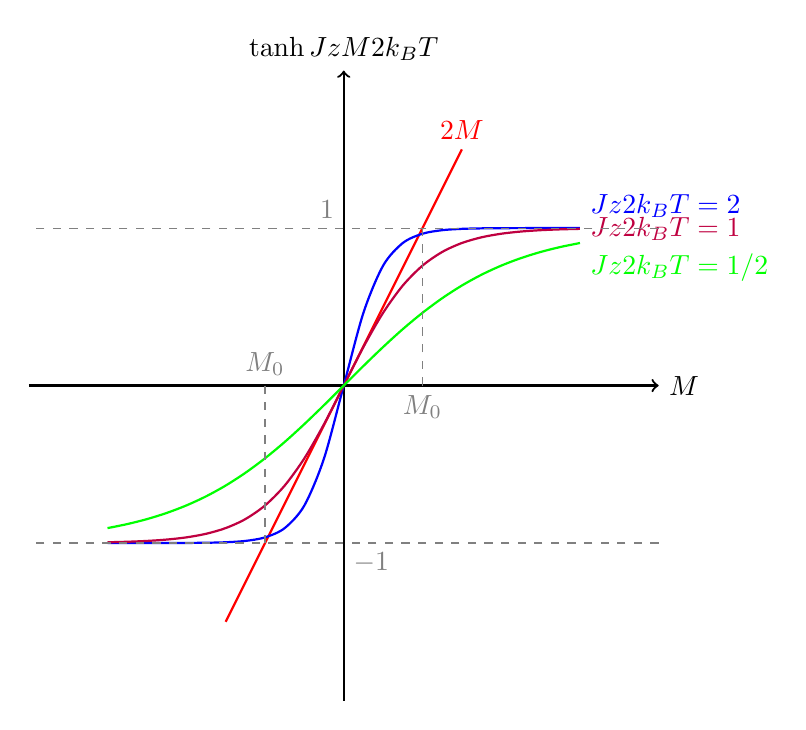
\begin{tikzpicture}
        \draw[thick, ->] (-4, 0) -- (+4, 0) node[right]{$M$};
        \draw[thick, ->] (0, -4) -- (0, +4) node[above]{$\tanh\f{\s J z M}{2 k_B T}$};
        \draw[thick, scale=1.0,domain=-1.5:1.5,smooth,variable=\M,red   ] plot ({\M},{2*\M}) node[above]{$2M$};
        \draw[thick, scale=1.0,domain=-3:3,smooth,variable=\M,blue  ] plot ({\M},{2*tanh(2*\M)}) node[above right]{$\f{\s J z}{2 k_B T} = 2$};
        \draw[thick, scale=1.0,domain=-3:3,smooth,variable=\M,purple] plot ({\M},{2*tanh(1*\M)}) node[right]{$\f{\s J z}{2 k_B T} = 1$};
        \draw[thick, scale=1.0,domain=-3:3,smooth,variable=\M,green ] plot ({\M},{2*tanh(1/2*\M)}) node[below right]{$\f{\s J z}{2 k_B T} = 1/2$};
        \draw[gray, dashed] (+1,0) node[below]{$M_0$} -- (+1,+2);
        \draw[gray, dashed] (-1,0) node[above]{$M_0$} -- (-1,-2);
        \draw[gray, dashed] (+4, +2) -- node[above left]{$1$} (-4, +2);
        \draw[gray, dashed] (+4, -2) -- node[below right]{$-1$} (-4, -2);
    \end{tikzpicture}
\end{center}
Evidently there are at most $3$ solutions depending on the temperature. There are three solutions if the slope of $\tanh \f{\s J z M}{2 k_B T}$ is greater than $1$ at $M = 0$. Taylor series,
\[ \tanh x \simeq x \]
Therefore the slope of $\f12\tanh \br{\f{\s J z M }{2 k_B T}}$ near $M=0$ is simply,
\[ \f{\s J z}{4 k_B T} \]
Therefore we define the critical temperature,
\[ \f{\s J z}{4 k_B T} > 1 \implies \f{\s J z}{4 k_B T_c} = 1 \implies T_c = \f{\s J z}{4 k_B} \]
Therefore we have the following case,
\begin{itemize}
    \item $T < T_c$ ferro-magnetism
    \item $T < T_c$ no ferro-magnetism
\end{itemize}
For iron we have $\s J \sim \SI{1}{\eV}$ and $T \sim \SI{e4}{\K}$. This is an example of a \term{phase transition}.
\begin{center}
    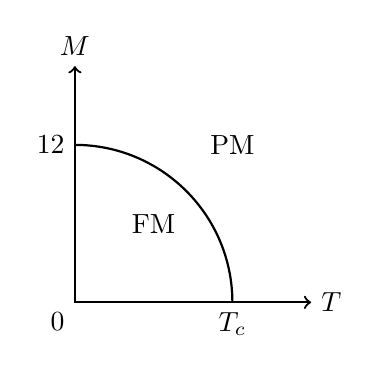
\begin{tikzpicture}
        \draw[thick,<->] (3, 0) node[right]{$T$} -- (0,0) node[below left]{$0$} -- (0, 3) node[above]{$M$};
        \draw[thick] (0,2) arc (90:0:2);
        \draw[thick] (2, 0) node[below]{$T_c$};
        \draw[thick] (0, 2) node[left]{$\f12$};
        \draw[thick] (1,1) node[]{FM};
        \draw[thick] (2,2) node[]{PM};
    \end{tikzpicture}
\end{center}
We refer to $M$ as the \term{M-order parameter} which allows us to formally distinguish between ferro-magnets and para-magnets. We have $M \neq 0$ in the FM phase but $M=0$ in the PM phase. \\

Depending on the nature of the phase transition boundary, we can have two types of phase translations: \term{first order phase translations} which are discontinuous or \term{second order phase transitions} which are continuous.

\begin{center}
    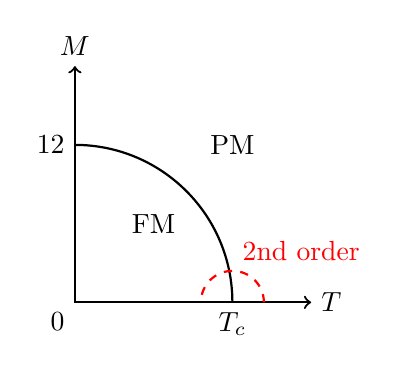
\begin{tikzpicture}
        \draw[thick,<->] (3, 0) node[right]{$T$} -- (0,0) node[below left]{$0$} -- (0, 3) node[above]{$M$};
        \draw[thick] (0,2) arc (90:0:2);
        \draw[thick,red,dashed] (2+0.4,0) arc (0:180:0.4) node[above right,midway]{2nd order};
        \draw[thick] (2, 0) node[below]{$T_c$};
        \draw[thick] (0, 2) node[left]{$\f12$};
        \draw[thick] (1,1) node[]{FM};
        \draw[thick] (2,2) node[]{PM};
    \end{tikzpicture}
    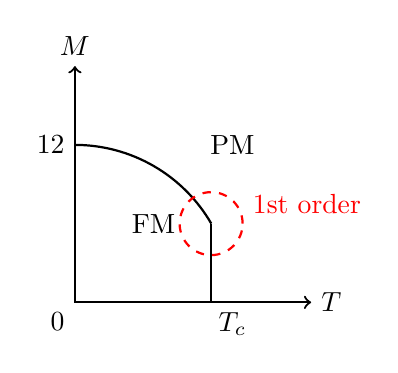
\begin{tikzpicture}
        \draw[thick,<->] (3, 0) node[right]{$T$} -- (0,0) node[below left]{$0$} -- (0, 3) node[above]{$M$};
        \draw[thick] (0,2) arc (90:30:2);
        \draw[thick,red,dashed] (1.73+0.4,1) arc (0:360:0.4) node[above right]{1st order};
        \draw[thick] (1.73, 0) -- (1.73, 1);
        \draw[thick] (2, 0) node[below]{$T_c$};
        \draw[thick] (0, 2) node[left]{$\f12$};
        \draw[thick] (1,1) node[]{FM};
        \draw[thick] (2,2) node[]{PM};
    \end{tikzpicture}
\end{center}





\end{document}

